%==================================================================================================
%   LUKES THESIS TEMPLATE 1.2
%   -------------------------
%   This template is based upon the offcial IMM PhD Thesis template, it is enhanced with a number
%   of new features and a number of errors have fixed. This template is intended to be complied to
%   PDF using PDFLATEX and is tested using the MiKTeX 2.9 LaTeX distribution.
%   It is based on the official DTU-IMM Thesis template by Finn Kuno Christensen in 2009.
%   Small bugfixes by Kasper Laursen in 2012 and 2013.
%   Small updates by Finn Kuno Christensen/Henning Christiansen in 2015.
%   -------------------------
%   Last Updated: 2015-01-08
%==================================================================================================
%
%==================================================================================================
% DOCUMENT SETUP
%==================================================================================================
\documentclass[10pt,twoside]{book}                  %Official DTU-IMM Thesis document setup
%
%Set to 'print' for printed version, use 'net' for online version
\def\thesisversion{print}
%
%==================================================================================================
% PACKAGES
%==================================================================================================
\usepackage{LukeThesis}                             %Import Thesis base style
%input{PhDMacros}                                   %Thesis specific macros
%
%==================================================================================================
% THESIS PROPERTIES (Modifiy these fields with your details)
%==================================================================================================
\def\thesisauthor{Anders Beck}                     %Author
\def\thesistitle{Gesture Based Input Method for Wearable Devices}               %Title
\def\thesishandin{02-July}                       %Submission date (Day-Month}
\def\thesisdegree{M.Sc.}                              %Degree ('B.Eng', 'B.Sc.', 'M.Sc.' or 'PhD')
\def\thesisyear{2018}                               %Submission year
\def\thesisnumber{????}                             %DTU-IMM Serial number (do not include year)
\def\thesisISSN{0000-0000}                          %ISSN number
\def\thesiskeywords{Keywords are, comma separated}  %PDF keywords
\derivethesisprops                                  %Derive dependent properties
%
%==================================================================================================
% SECTION NUMBERING SETUP
%==================================================================================================
\setcounter{tocdepth}{2}                            %2 adds sections up to subsections
\setcounter{secnumdepth}{3}                         %Subsubsections get a number when this is 3
%
%==================================================================================================
% THESIS STRUCTURE  (Modifiy to include more chapters etc)
%==================================================================================================
\begin{document}
%------------------------
%Pre-frontmatter material
%------------------------
\prefrontmatter
%--------------------
%Frontmatter material
%--------------------
\frontmatter
\pagenumbering{roman}                               %Set frontmatter numbering style
\chapter{Summary (English)}

The goal of the thesis is to ...                                   %English summary of Thesis
\markboth{}{}                                       %Set headings (left)(right)
\chapter{Summary (Danish)}
\begin{otherlanguage}{danish}

Målet for denne afhandling er at ...

\end{otherlanguage}                                   %Danish summary of Thesis
\markboth{}{}                                       %Set headings (left)(right)
\chapter{Preface}

This thesis was prepared at DTU Compute in fulfillment of the requirements for acquiring an M.Sc. in Engineering.

The thesis detail the design and implementation of a wristband device and companion app for manual collection of data on subjective experiences using a gesture based system. An experiment was conducted in order to compare the performance of the wristband with a touch screen implementation of a Visual Analogue Scale.

%==================================================================================================
% SIGNATURE AREA
%==================================================================================================
\vspace{20mm}
\begin{center}
    \hspace{20mm} Lyngby, \thesishandin-\thesisyear
    \vspace{5mm}
    \newline
  %Update signature image file in line below
    
\includegraphics[scale=0.3]{Signature.png}
\end{center}
\begin{flushright}
    \thesisauthor
\end{flushright}
% % % EOF % % %                                     %Preface
\markboth{}{}                                       %Set headings (left)(right)
\chapter{Acknowledgements}

First I'll like to thank my supervisor Jakob Eg Larsen for suggesting me the topic for this thesis. Furthermore I want to thank him for his guidance, feedback and engagement throughout.

Thanks to everyone that volunteered their time to participate in the experiment.

Thanks to my friends, family and former colleagues at IBM for support and their feedback to this thesis. A special thanks to my friends and colleagues Morten Due Christiansen and Alexander Lillelund for all their help and feedback in the development process.                            %Acknowledgements
\markboth{}{}                                       %Set headings (left)(right)
%------------------
% Table of contents
%------------------
\newpage\mbox{}\newpage
\chaptermark{Contents}
\pdfbookmark{\contentsname}{toc}
\renewcommand{\sectionmark}[1]{\markright{#1}}
\sectionmark{Contents}
\addtolength{\parskip}{-\baselineskip}
\tableofcontents
\addtolength{\parskip}{\baselineskip}
\renewcommand{\sectionmark}[1]{\markright{\thesection\ #1}}
%-------------
% Main content
%-------------
\mainmatter
\chapter{Introduction}

Background, explain the problem..


\begin{figure}[h!]
    \centering
    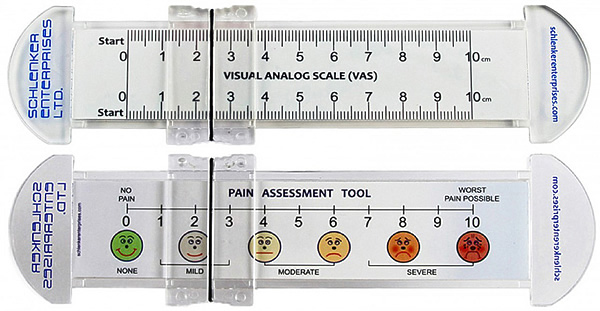
\includegraphics[width=1\textwidth]{figures/real_vas.jpg}
    \caption{VAS Pain Scale Ruler\cite{real_vas}}
    \label{real_vas}
\end{figure}

\section{Thesis Goals}

Propose the solution?

\section{Contributions}

\section{Thesis Structure}                                  %Chapter 1
%\include{Chapter2}                                 %Chapter 2
\chapter{Related Work}

TODO: Introduction for this section. 

\section{Reducing the burden of self tracking}
Self tracking can solve the problem of memory recall bias, by letting the user register observation in the moment (or very close to) they occur. But requiring the user to log observation introduces a burden of the work involved in doing so. As mention traditionally this has been done with pen and paper, but with the invention of smartphones and smartwatches this burden can be reduces. The work of Ponnada et al., 2017\cite{compare} investigate the interruption burden with both smartphones and smartwatches when used to with both regular EMA and $\mu$EMA. The difference between EMA and $\mu$EMA is that EMA will prompt the use less than $\mu$EMA, but requires the user to answer several questions back to back, where $\mu$EMA will instead prompt the user much more frequently, but only require the user to answer one question, which can be answered on the same screen showing the question. 

In a prior 4 week pilot study Ponnada et al. found that smartwatch $\mu$EMA demonstrated higher response rates and participants reported a lower perceived burden than smartphone EMA, even though the interruption rate for smartwatch $\mu$EMA was 8 times higher than smartphone EMA. In a new 4 week study they gathered data based on a smartwatch EMA in order to determine if the previous result where due to the fact that the data was gathered on a watch, or if it in fact was due to the $\mu$EMA. Their results showed that there were no statistically significant differences in compliance, completion, and first-prompt response rates observed between smartphone EMA and smartwatch EMA. But smartwatch $\mu$EMA response rates where significantly higher than smartwatch EMA. Their results suggest that the higher compliance and lower perceived burden is more likely to do with $\mu$EMA than the device itself and that compliance with EMA may not improve simply by changing the device.

The work of Ponnada et al. only looked into EMA where the device prompts the user for information, not situations where the user registers an observation. In his thesis Kami\'nski, 2016\cite{tomas} investigates how to enable self logging with different forms of input: a binary sample, selection input form a list, VAS and a numerical scale. He designed and implemented all of the input methods onto a smartwatch, where on the watch face each method input method could be selected. In figure \ref{tomas_design} we can see his design, the watch face has a shortcut for each input method. In figure \ref{tomas_design2} we see how the interaction occurs, and that it takes 1-3 touches to log the desired data depending on the input method.

\begin{figure}[h!]
    \centering
    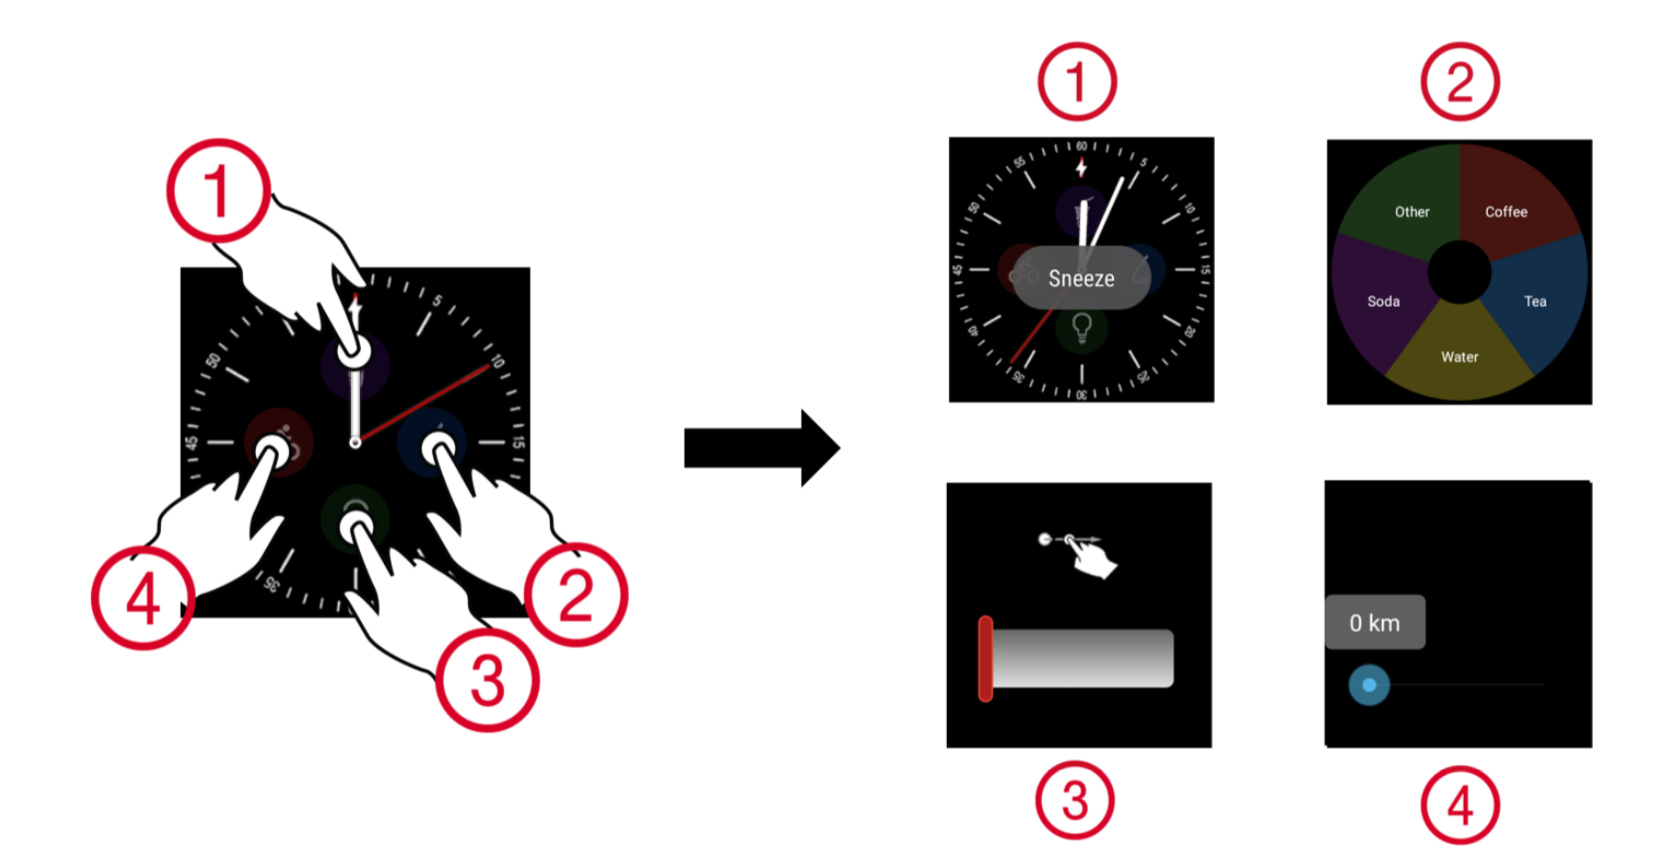
\includegraphics[width=1\textwidth]{figures/tomas_design.png}
    \caption{Design for self logging on a smartwatch by Kami\'nski\cite{tomas}}
    \label{tomas_design}
\end{figure}

\begin{figure}[h!]
    \centering
    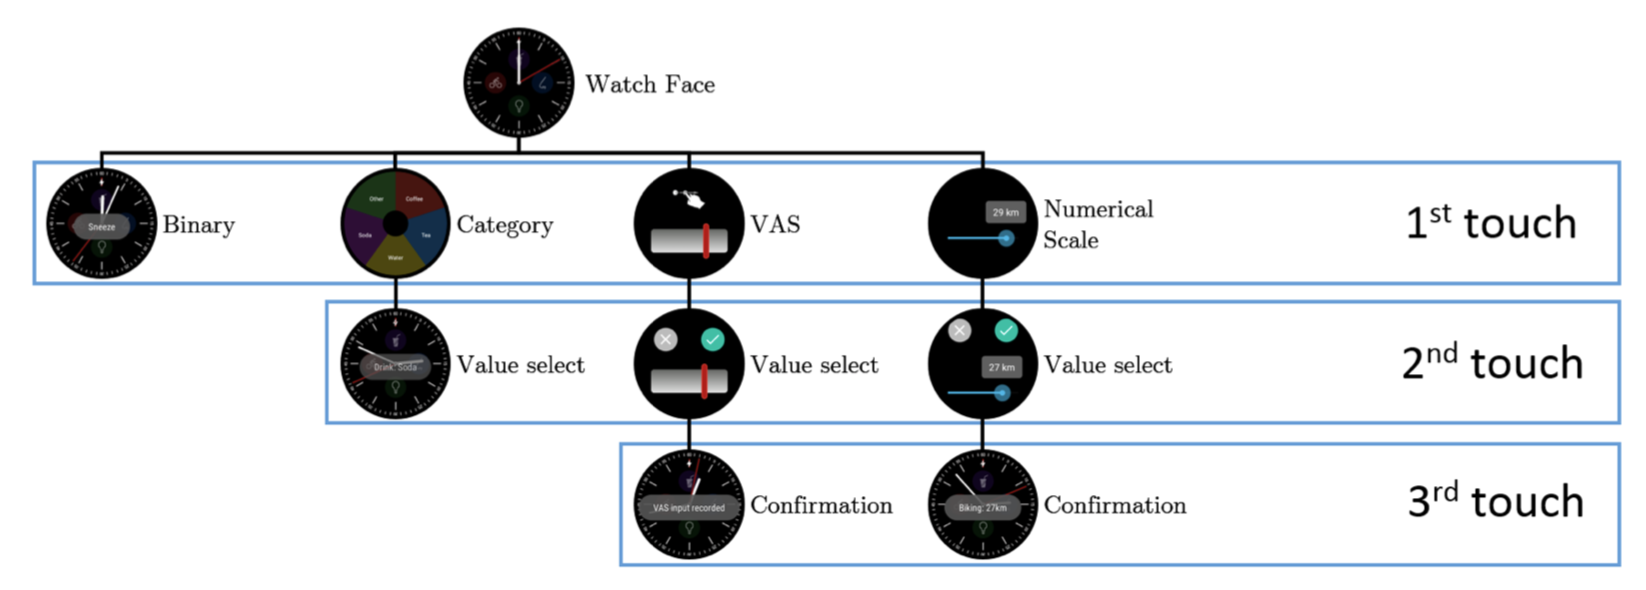
\includegraphics[width=1\textwidth]{figures/tomas_design2.png}
    \caption{Interaction for self logging on a smartwatch by Kami\'nski\cite{tomas}}
    \label{tomas_design2}
\end{figure}

For comparison Kami\'nski also implemented his a similar design on a smartphone following the \emph{Android material design guide}\cite{android_design} and conducted an experiment where he compared the two devices performance (interaction time, lower is better). His result showed a reduction in the user interaction time by approximately 30\% on average, thus successfully reducing the burden related to self logging. Beside his experiment Kami\'nski also had himself and to others use his design to collect data about their daily life (sneezing, skin itching and water consumption) over a 13-21 week period. What he found was a high compliance rate, all though it is a fairly biased test, since all three participants where involved in the project and are working with self logging technologies on a daily basis. 

Even though Kami\'nski design was a success, there persist an underlying problem with smartwatches; that they still require the user to user to activate them (often by tapping the screen or rotating their arm) and then the user has to look at the screen to touch the right section to register the input. Dam-Jensen, 2018\cite{dam} investigates this issue in his thesis. He introduces three ways of performing self logging, all using a \say{smartbutton} (wireless button connected to smartphone/smartwatch) to achieve a display-less logging system. The three input method that Dam-Jensen designed was:

\begin{enumerate}
	\item Hold Button: Measure the time the button is held down.
	\item Rotate Lower Arm: Using the built in gyroscope in the smartbutton, the difference in rotation from when the button was pressed to it was released is measured. In order to achieve a measurement the user would hold the button in the hand, rotate the lower arm to a neutral position, hold down the button, rotate the lower arm to the end position and release the button. 
	\item Rotate Upper Arm Around Elbow: Similar to the previous method, but instead of rotating the lower arm, the user would raise/lower his/hers upper arm around the elbow.
\end{enumerate}

For a comparison baseline method a standard VAS was used. In order to compare his three methods to the VAS Dam-Jensen conducted an experiment based on the work of Matejka et al., 2016 \cite{grey}, where participants are asked to rate a color between white and black on a grey scale where the colors are equally spaced out on the CIELAB color space\cite{cielab} (more on this later). His results showed that there where no significant difference in accuracy between his three designed input methods compared and the baseline, thus meaning that all three methods are viable and could be used for self logging, and in their simple nature can reduce the burden on the user.

\section{Long term use of self logging}
As mentioned Ponnada et al. conducted two 4 weeks studies with EMA and $\mu$EMA and Kami\'nski conducted a even longer 13-21 week use case where three people used his design to track daily activities. Both Ponnada et al. and Kami\'nski work show great potential for real use, but none of them has been proper tested in the real world, also none of them utilizes a device similar to that of Dam-Jensen's work, where there is no screen and only a single button for registering observations.

In a case study Larsen et al., 2017\cite{eg} investigated the real life use case of a novel device for self logging. They had a Danish veteran suffering from post-traumatic stress disorder equipped with a \say{smartbutton}, that when pressed will store a time stamp. By connecting a smartphone the data can be transferred from the smartbutton to a data file for further analysis. The veteran was then instructed to press the button whenever he experienced a specific event related to his PTDS (the \say{trigger event} was chosen based on a two-hour assessment interview together with his therapist). The veteran wore smartbutton for 100, pressing the button whenever he experienced the specific event.

The results showed that the veteran had a high compliance, actively using the device throughout the 100 days (due to a technical issue no data was collected during the second week). The data collected revealed patterns that explained why/when the veteran's events would be triggered, which would not have revealed itself from the conversational assessment. In other words, not only was it a success from a technical and usability standpoint, but it also succeeded in bringing valuable new information to the treatment process. 

\section{Comparing ratings of behavior}
When developing new methods for self logging it is important to access the feasibility of these methods. As mentioned Kami\'nski did this simply by comparing the user interaction time, while Dam-Jensen did a more comprehensive comparison by looking into how precise the data recorded with his designs compared to the VAS. He did by having his participants rate shades of grey with the different input methods. That experiment was inspired by the work of Matejka et al., 2016 \cite{grey} where they investigate the bias of different slider designs. In order to do so they base their experiment on the work of Borg and Borg, 1991\cite{borg} that extensively studied using a \say{scale of blackness} as a stimulus and concluded that it serves as a good test of general rating behaviour, and further more it provides a truth value (the color displayed) with can be compared to the response rating from the participant. Matejka et al. designed their experiment to test severely different slider designs with various combinations of labels, tick marks and bands. In figure \ref{mate_ex} a design with 2 labels and 5 ticks is shown. Matejka et al. recruited participants via \emph{Amazon Mechanical Turk}\cite{turk}. Participants where then showed one of the 50 shades of grey (as seen in figure \ref{50shades}), then asked to rate the color from white to blakc using the slider. This process was repeated several 50 times so each participants was exposed to all the shades of grey (in random order), this was then repeated until the participants had been exposed to each shade of grey 4 times, 200 trials in total. Each participant was only exposed to one slider design, and was afterwards excluded to participate further. 

\begin{figure}[h!]
    \centering
    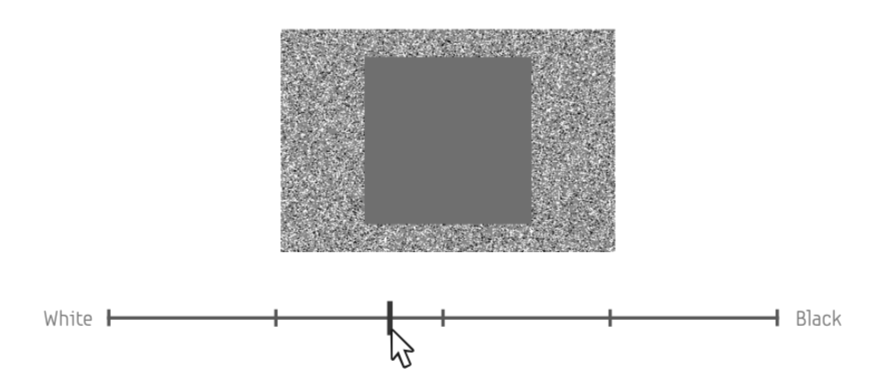
\includegraphics[width=1\textwidth]{figures/mate_ex.png}
    \caption{Slider bias experiment by Matejka et al.\cite{grey} with 2 labels and 5 ticks}
    \label{mate_ex}
\end{figure}

\begin{figure}[h!]
    \centering
    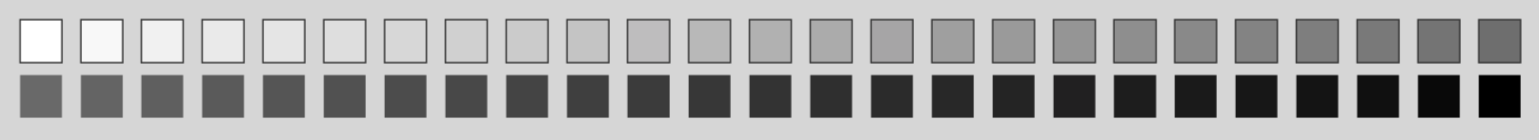
\includegraphics[width=1\textwidth]{figures/50shades.png}
    \caption{50 shades of grey used by Matejka et al.\cite{grey}}
    \label{50shades}
\end{figure}

With their results they investigated the bias for each slider design by looking at the distribution of responses and calculating a \say{smoothness} value representing the bias as well as precision and response time. Their results showed that sliders with ticks introduces the most bias towards the tick marks, followed by sliders with many labels and combination of the two. Banded sliders showed only small amount of bias and sliders with only two labels showed the least amount of bias. The higher amount of both ticks and labels resulted in higher precision.

\section{Relation to this thesis}
The work of Ponnada et al., Kami\'nski and Dam-Jensen all point towards the benefit reducing the burdens and show. Their work has been a great inspiration for this thesis, together with Larsen et al. work showing the real world benefit of in situ measurements. This thesis will further investigate two of Dam-Jensen's designs, the \say{Rotate Lower Arm} and \say{Rotate Upper Arm Around Elbow} methods together with the \say{rating of blackness} will be the starting point.
\chapter{Analysis}\label{anal_ch}

\section{Self tracking}
%\textbf{COMMENT: Elaborate this to motivate the project and explain the background.}
Experience Sampling Method (ESM) and Ecological Momentary Assessment (EMA) are the research methodologies that refer to the usage of self tracking\cite{esm}. What defines these methods are the use of collecting real world data in the moment, whether that be psychological (thoughts, feelings, mood, pain etc) or physical (food/drinks consumed, sneezing, cramps etc). Traditionally this had been achieved with diaries, which could have the same set of questions printed on each page designed to collect the desired data. In modern times digital diaries have been created, for example as apps on smartphones and smartwatches. The benefit of these methods is that the prevent recall bias, since the data is collected in the moment (or shortly after) compared to daily diaries where a user by the end of the day has to think back and recall the data. The more time passed between the event and the time the data is collected, the larger the risk of recall bias will be, and the data can even be forgotten.

When collecting data that requires active self tracking, there will always be a burden involved. The simpler the data is to collect, the smaller the burden can be. For example tracking each time a person sneezes only requires a time stamp which can be collected by wearing a smartbutton like the one made by Larsen et al.\cite{eg}. On the other hand, if tracking the pain levels of a patient, the patient needs a way to input that on scale preferably a VAS. One solution has been to create a digital VAS on a smartphone or smartwatch, similar to the work of Kami\'nski\cite{tomas}. Compared to the smartbutton, this solution has a much higher burden, the user must turn the display on, navigate the software to input the value and it requires a user's full attention to execute. With the improvements Dam-Jensen\cite{dam} introduced, the burden was lowered to only have the user press, hold and release a button while doing an arm gesture.

As a evolution to the design of Dam-Jensen\cite{dam}, this thesis will introduce a self tracking method where the user will follow the same gestures (described later in this Chapter) and press a button only once (not press, hold and release). This new method will reduce the burden even further compared to the other mentioned methods.










\section{Usage of VAS}
In Figure \ref{real_vas} we see one of the VAS rulers that is sold to and used by hospitals to measure the pain levels of patients, while they come in different designs their principals are the same. On one side of the ruler we see 5-6 faces with expression going from happy to discomfort to sad and crying, these expression are meant to illustrate the amount of pain and are often displayed together with a text description explaining the feeling of pain as seen in Figure \ref{vas_faces}. On the other side of the VAS ruler there is regular ruler of 10cm (sometimes shown as 100mm instead). On the ruler there is a slider, the patient will be shown the side of the ruler with the faces, and asked to adjust the slider to fit the level of pain they experience, on the backside the slider will indicate a position on the ruler from 0 (no pain) to 10 (most pain), this position is then registered by a doctor or nurse as the pain level. The VAS is not limited to measuring pain, it can be used for any subjective characteristics or attitudes that cannot be directly measured, for example mood, annoyance, anxiety, but the measuring of pain is the most common use of VAS.

\begin{figure}[h!]
    \centering
    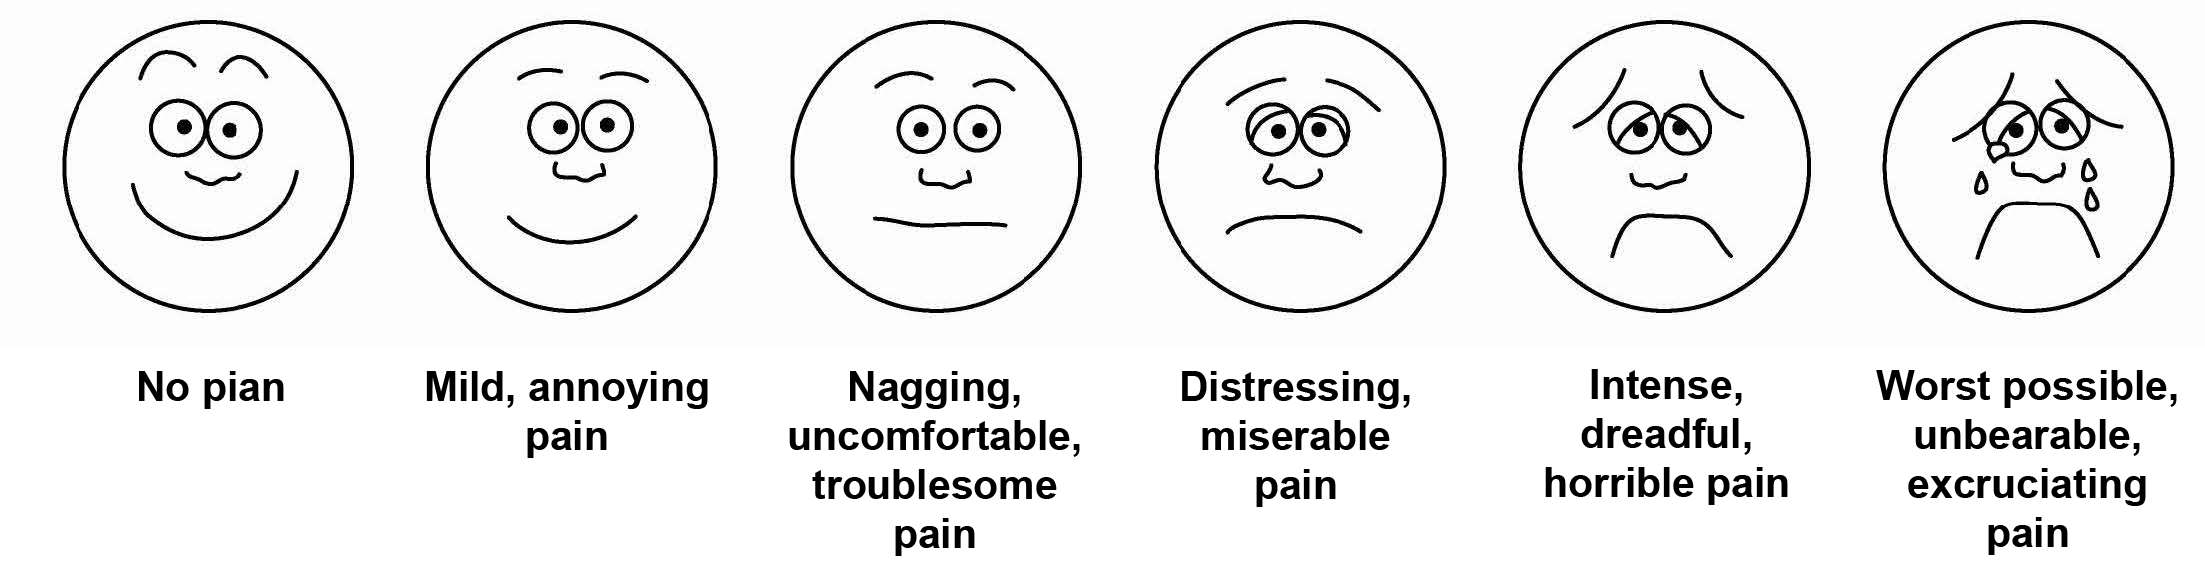
\includegraphics[width=0.75\textwidth]{figures/vas_faces.png}
    \caption{Example of faces and descriptions on VAS for measuring pain\cite{vas_faces}}
    \label{vas_faces}
\end{figure}

The VAS can be compared to the Likert scale\cite{likert} and Borg scale\cite{borg_scale}, but what makes the VAS different is that it is continuous where the others are discrete. Evidence show that VAS have better metrical characteristics compared to discrete scales and therefor a wider range of statistical methods can be applied to the measurements\cite{best_scale}.

Despite its benefits VAS are a burden to use, even digital version since the require a screen and attention. It is therefor interesting to investigate if other solutions with less burden can perform equally or better than the VAS.








\section{Orientation in 3D space}
Before creating a device that translates the orientation of the hand to a scale, one must first understand orientation in 3D space. We can rotate an object around each of its 3 axis, these actions are refereed to as pitch, roll and yaw. In Figure \ref{plane} we see an illustrations of these rotations performed on a airplane.

Pitch is rotation around the axis across the airplane, this rotation can be felt during takeoff and climbing (shortly after the wheels lift of the ground) of a airplane, where the pitch is dramatically changed from 0º (parallel to the ground) to $\thicksim$15-20º\cite{takeoff}.

Roll is rotation around the axis along the airplane, this rotation can sometimes be felt when an airplane has to perform a sharp turn and then rolls a little to one side so one wing tip is higher in the air than the other (when airplanes turn the yaw will also change), this rotational movement where the airplane rolls over is the roll axis.

Yaw is the rotation around the last axis, the same axis you would measure the height of airplane on. This rotation is barely felt in a airplane, but it is this orientation that will change the direction of the airplane, from lets say facing north to facing west by rotating 90º to the left (from the pilots perspective).

Getting the orientation of an object is then a matter of measuring the pitch, roll and yaw, there a different ways to do this and they will be discusses a little later, for now we will measure each rotation in degrees and define the orientation of 0º pitch, 0º roll and 0º yaw to be an object that is level in both directions and facing north. A full rotation in one axis is 360º and would leave the object in the same position as it started out. This definition is very similar to Euler angles witch will be discussed further.

\begin{figure}[h!]
    \centering
    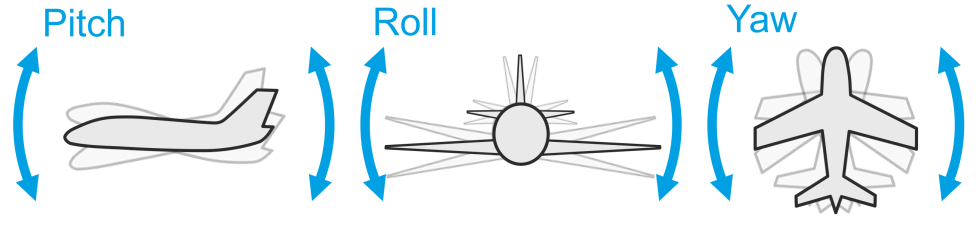
\includegraphics[width=1\textwidth]{figures/pitch_rool_yaw_v2.png}
    \caption{Pitch, roll and yaw of an airplane (edited version of figure found online\cite{plane})}
    \label{plane}
\end{figure}

\subsection{Orientation of the arm}
With the orientation defined as the rotation of the three axis, we need to translate this into movement of the arm. In Figure \ref{pitch}, \ref{roll} and \ref{yaw} the movement to adjust pitch, roll and yaw is described.

Pitch is changed by rotating the arm around the elbow, resulting in the lower arm being raised/lowered. The angle between the lower arm and table (horizontal plane) is then the measurement for this rotation.

\begin{figure}[h!]
    \centering
    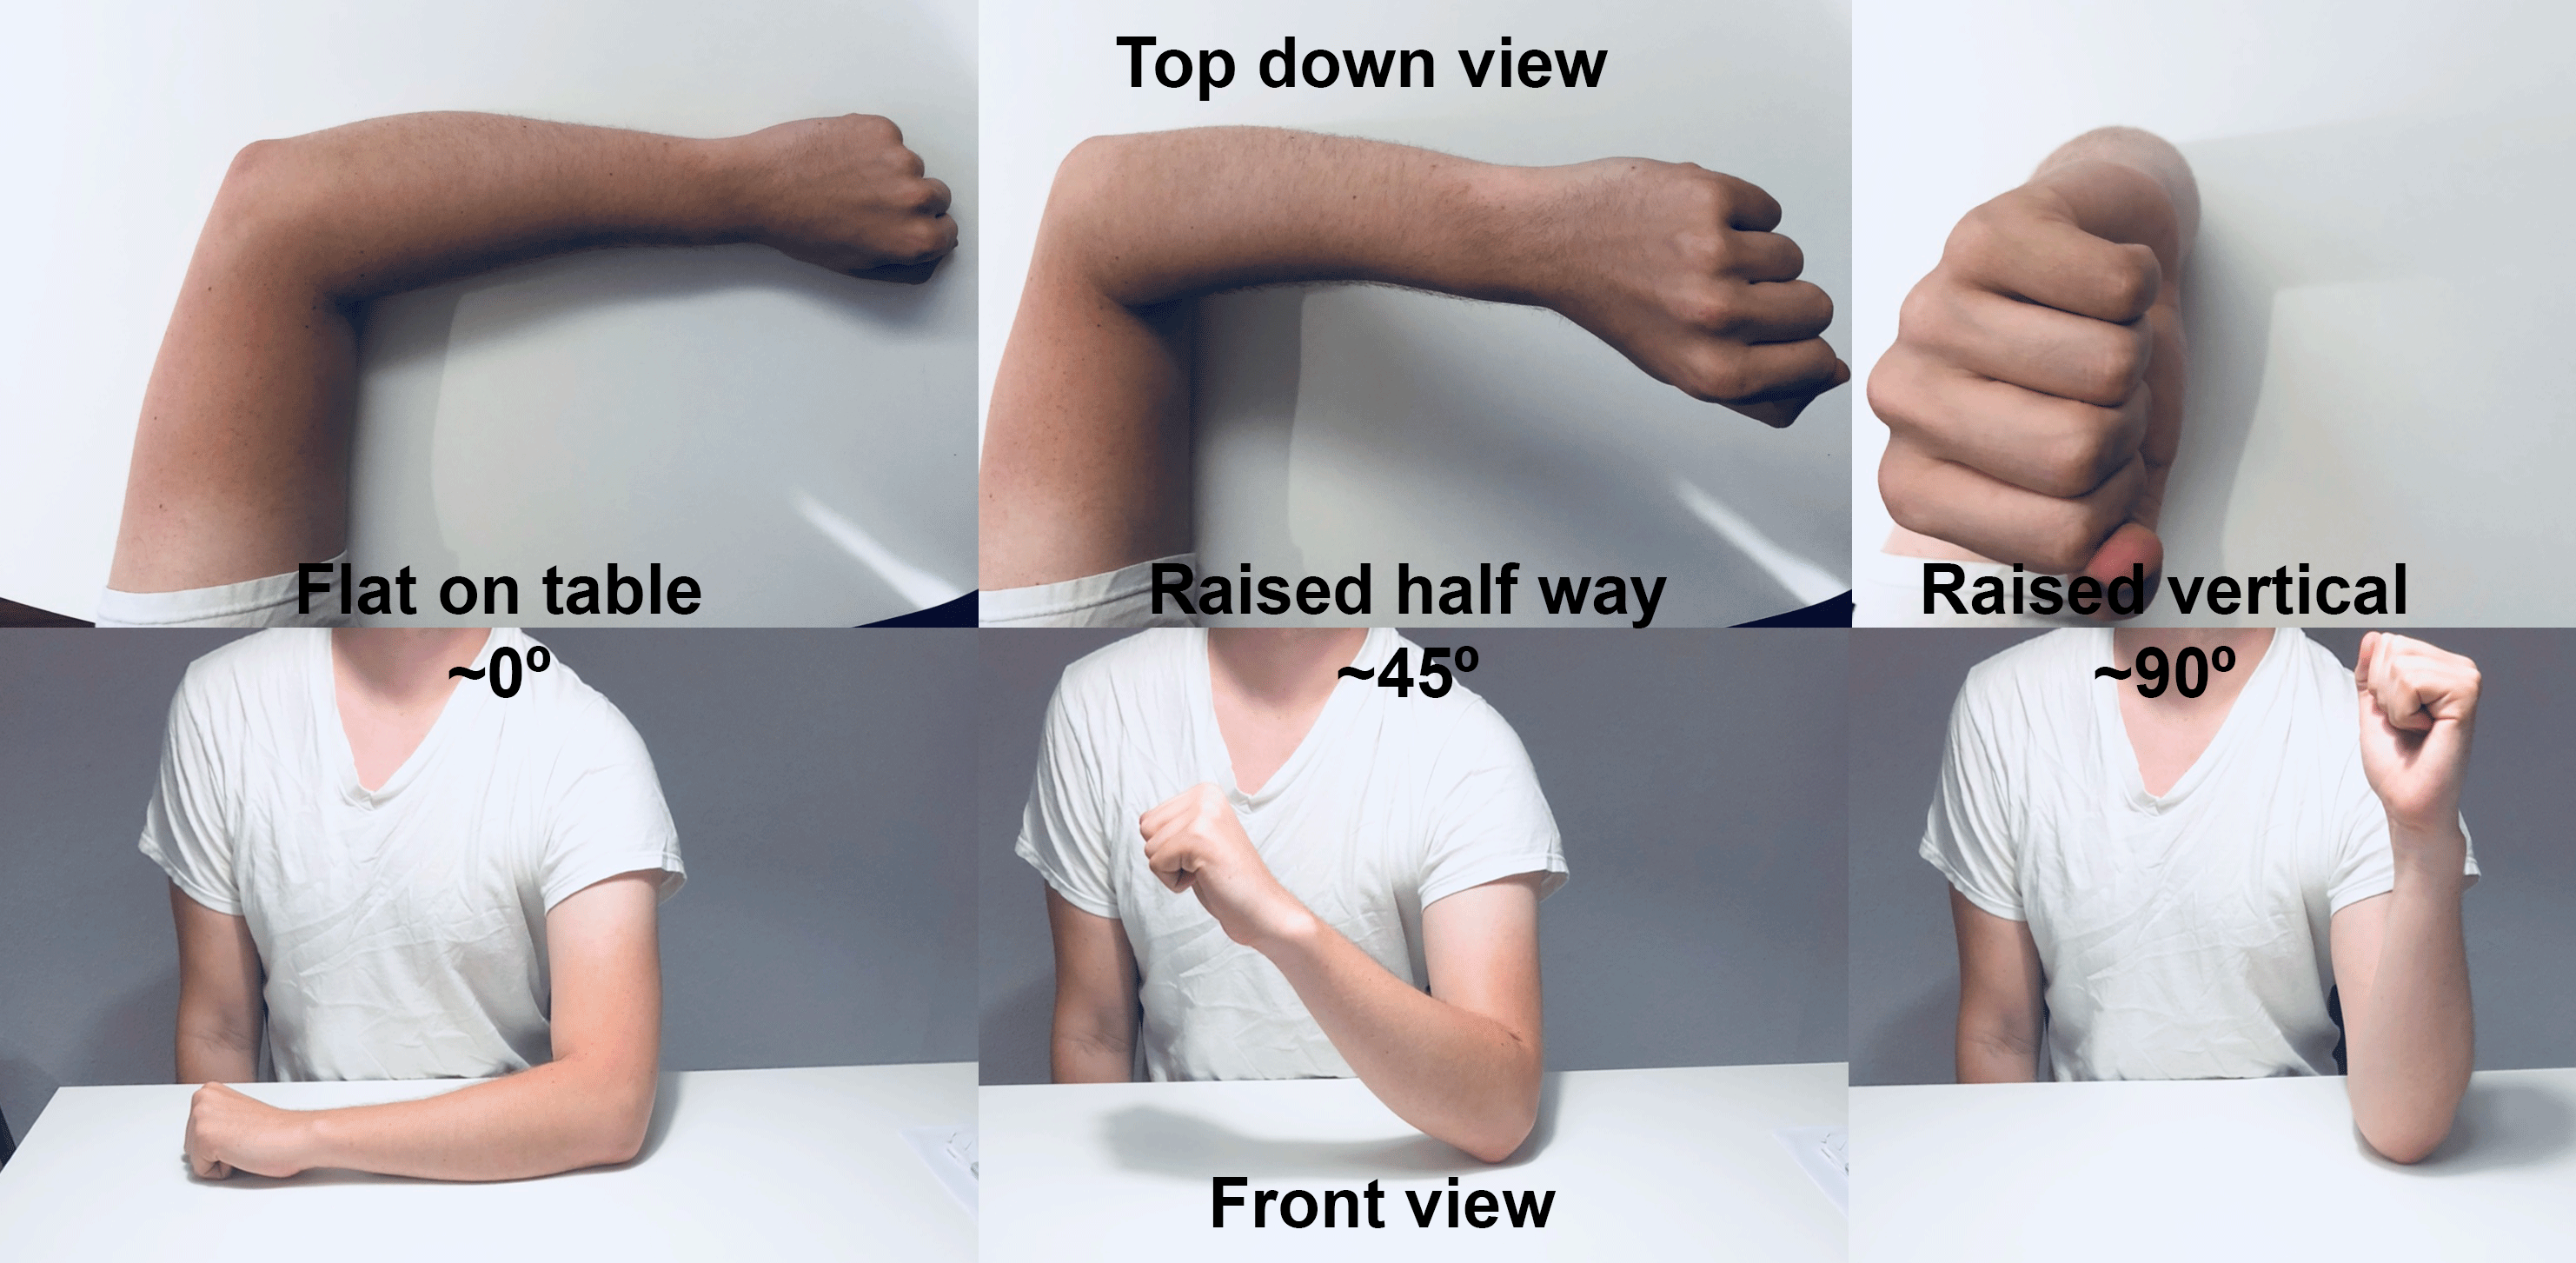
\includegraphics[width=1\textwidth]{figures/pitch.png}
    \caption{The movement for adjusting \underline{pitch} by rotating the arm around the elbow}
    \label{pitch}
\end{figure}

Roll is changed by rotating the wrist/lower arm, the angle between the back of the hand and table is then the measurement for this rotation.

\begin{figure}[h!]
    \centering
    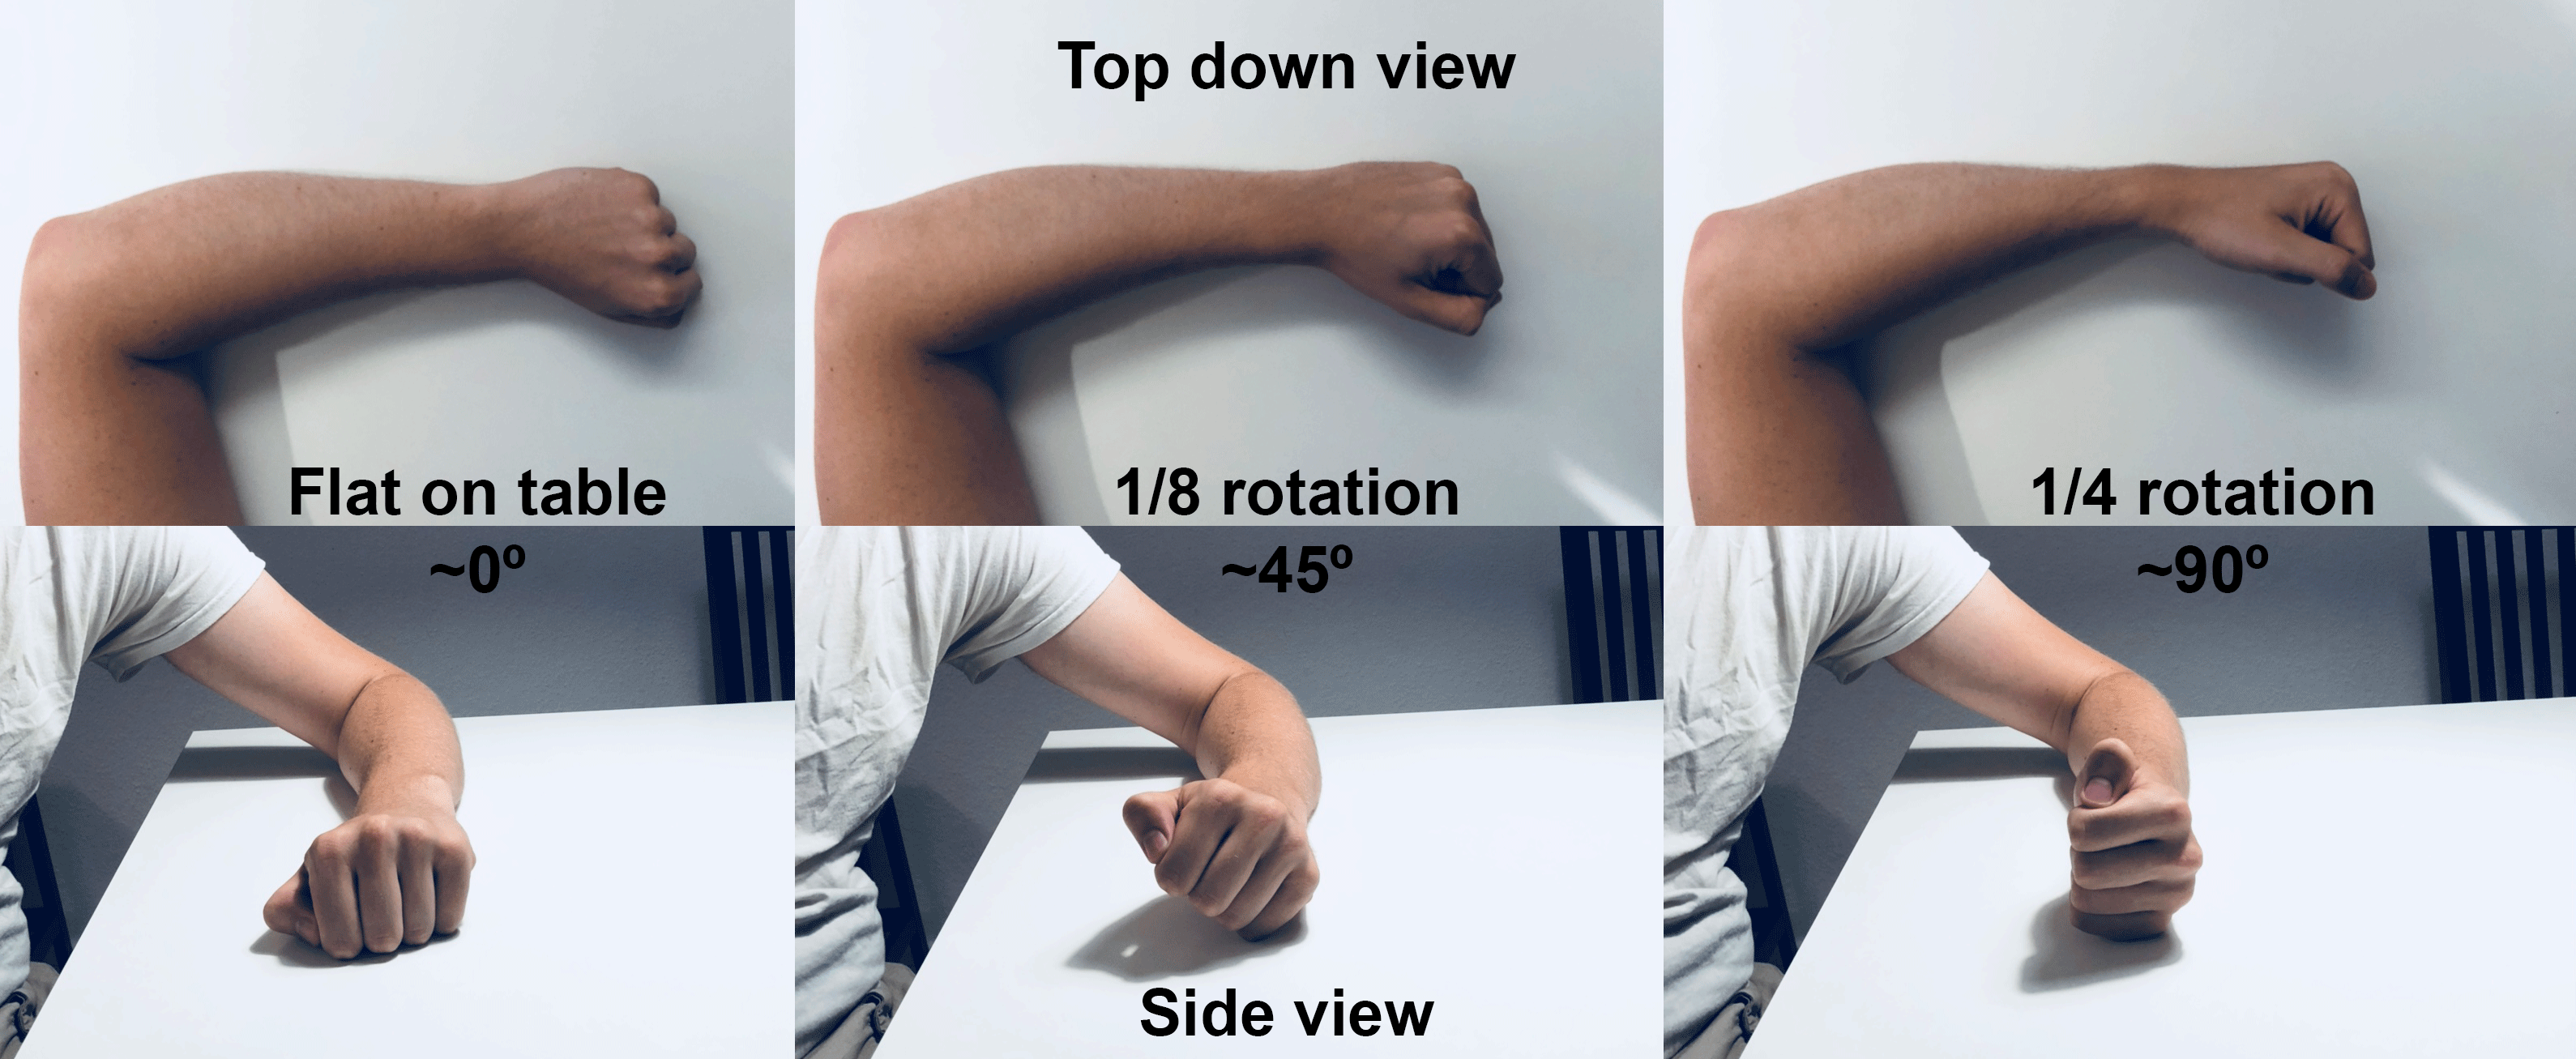
\includegraphics[width=1\textwidth]{figures/roll.png}
    \caption{The movement for adjusting \underline{roll} by rotating the wrist/lower arm}
    \label{roll}
\end{figure}

Yaw is changed by bending the lower arm the elbow, keeping it level with the table, thus changing the direction of the lower arm. The angle of direction is then the measurement for this rotation.

\begin{figure}[h!]
    \centering
    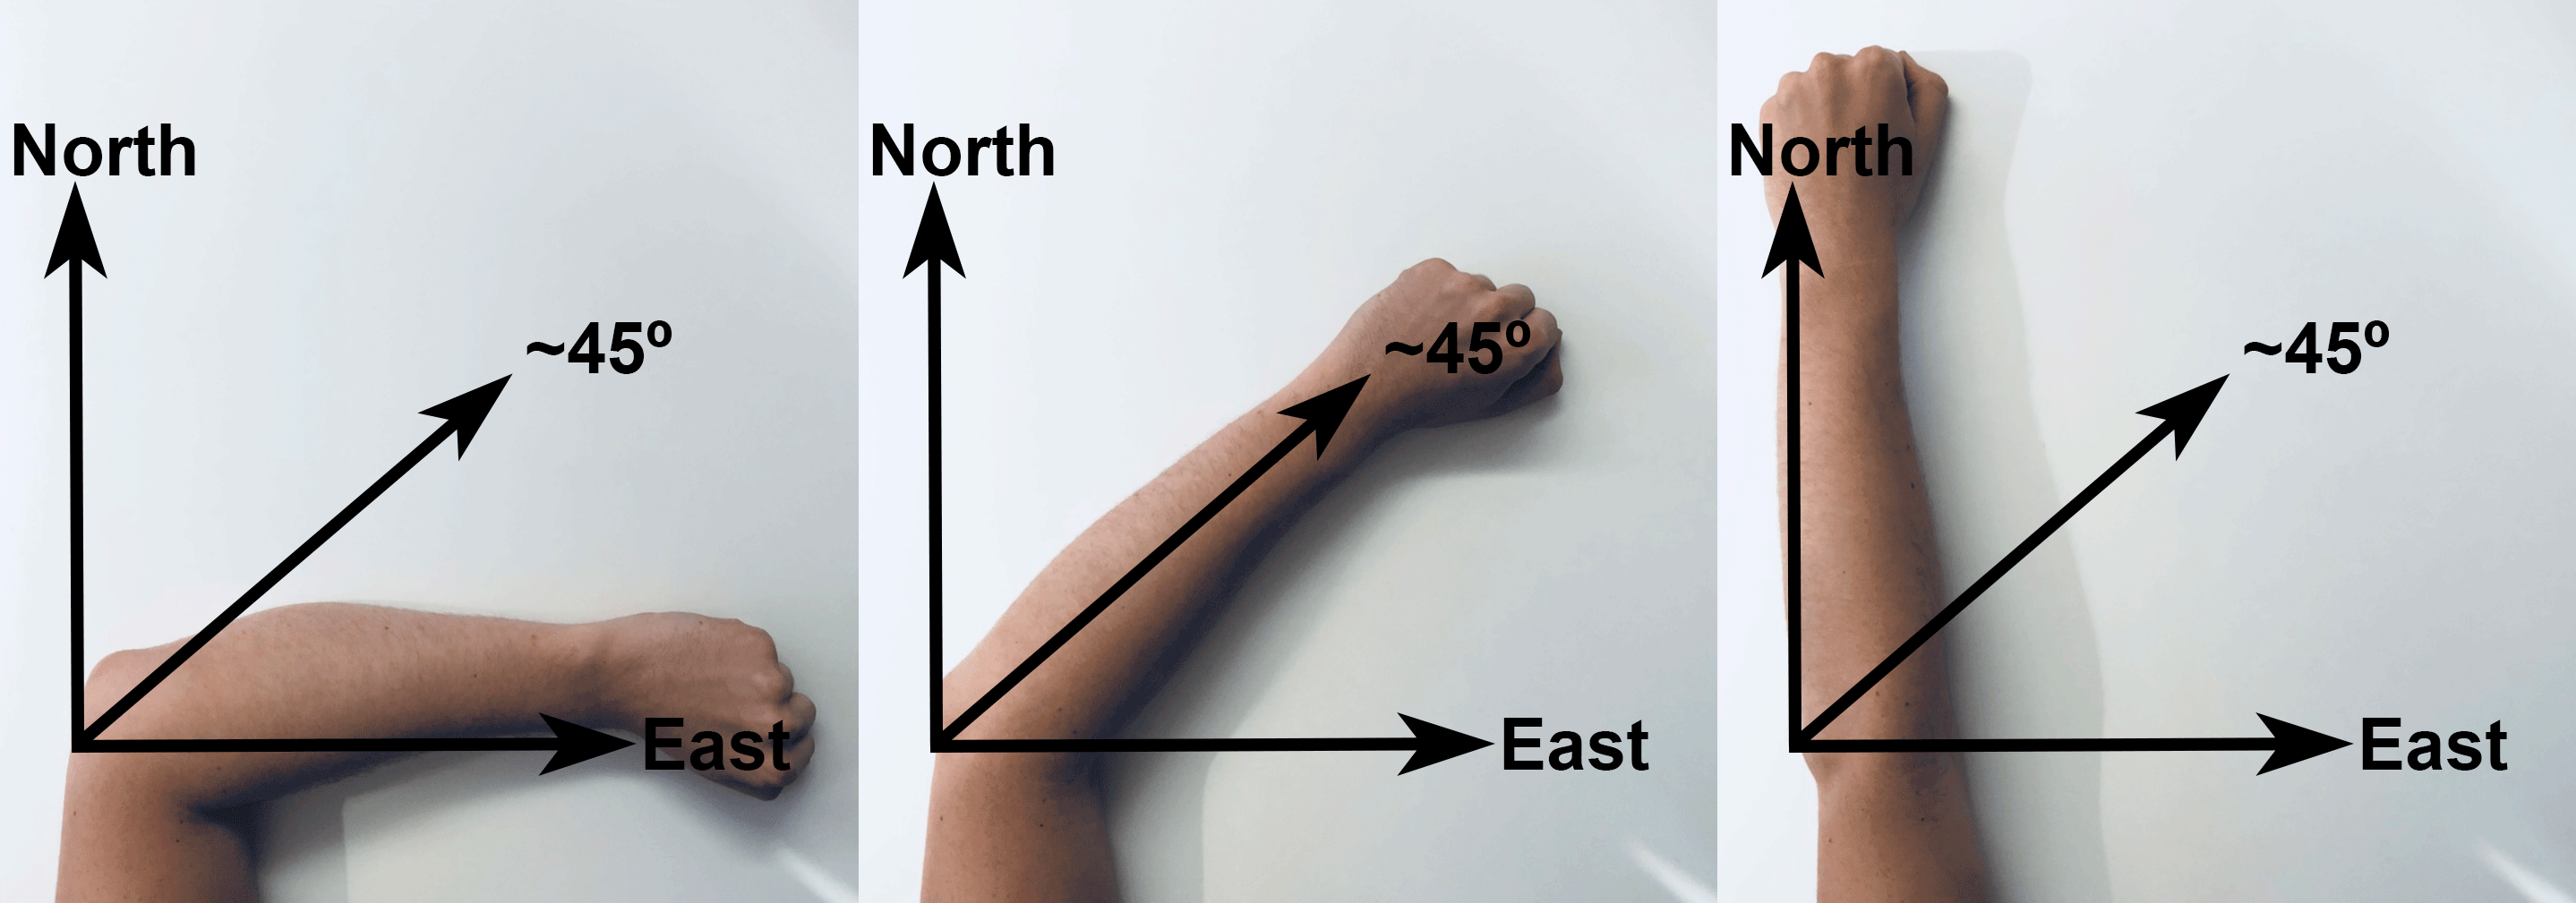
\includegraphics[width=1\textwidth]{figures/yaw.png}
    \caption{The movement for adjusting \underline{yaw} by rotating the lower arm around the elbow (note the arm is flat/horizontal on the table)}
    \label{yaw}
\end{figure}

Of course all three rotation can be achieved in other ways, for example yaw can be changed by turning the entire body to face another directions. But for the purpose of this thesis we look at these motions because they are done in front of one self, can be executed both while sitting at a table (for best reference) or while standing, and for all these motions the body itself also is a reference point, where turning your entire body would require another reference point to make sense of the scale.

\subsection{IMU}
\textbf{COMMENT: Get a illustration of the BNO055 or specs. Mention processing of data required - calibration issues.. Drift experiment}

In order to measure the orientation we will mount a device on the wrist which contains an IMU from which the orientation can be read. Most IMUs are equipped with accelerometers, gyroscopes and magnetometers and offers either raw sensor values or the calculated Euler angles and quaternions for absolute orientation. In it self the raw sensor values can't provide the orientation, since it measures the change for example will the gyroscope alone measure the rate of rotation witch in it self can't lead to an absolute orientation. But together the sensors provide enough data that this can be calculated. The IMU will use its magnetometer to find north and use this to calibrate yaw, using its accelerometers the IMU can measure gravity and calibrate both pitch and roll. All together this lets the IMU calculate the absolute orientation. These calculations also requires the IMU to be calibrated and if not done correctly this can lead to issues, such as drift, where the orientation values will change even though the IMU sits completely still. 

To demonstrate this, a test was preformed with the Adafruit 9-DOF Absolute Orientation IMU Fusion Breakout - BNO055\cite{gyro}, logging the Euler angles with and without calibration while the IMU sat completely still. Once every minute the Euler angles was read from the IMU and logged to a file, two trials where run for nine and twelve hours respectively without and with calibration. The results can be seen in Figure \ref{drift1} and \ref{drift2}, we see that without calibration the sensor drifts and the Euler angles change quite dramatically over time, while with calibration the Euler angles only had minor change.

\begin{figure}[h!]
    \centering
    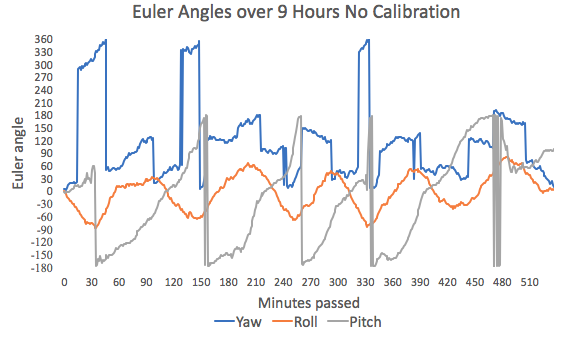
\includegraphics[width=1\textwidth]{figures/drift1.png}
    \caption{Reading the Euler angles from the BNO055 IMU\ref{gyro} without calibration}
    \label{drift1}
\end{figure}

\begin{figure}[h!]
    \centering
    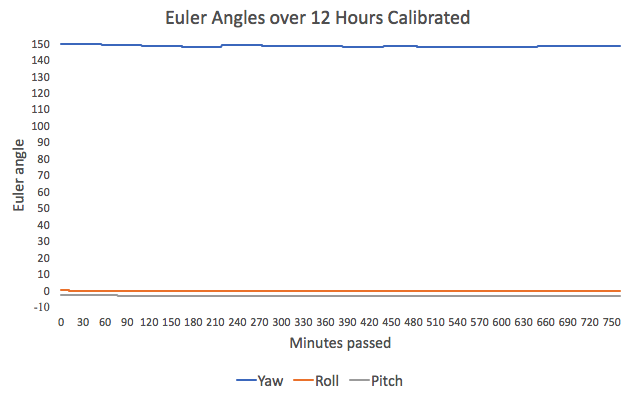
\includegraphics[width=1\textwidth]{figures/drift2.png}
    \caption{Reading the Euler angles from the BNO055 IMU\ref{gyro} with calibration}
    \label{drift2}
\end{figure}


The most common ways to represent absolute orientation is using either Euler angles\cite{euler} or quaternions\cite{quat}. Euler angles describes the orientation by angles of the 3 axis, this is the most intuitive approach but it has it downfall. When two of the gimbals in a gyroscope align into a parallel configuration, then one of the three degrees of freedom is lost, this is called Gimbal lock\cite{gimbal}. When Gimbal lock occurs changes in the locked axis cannot be measured, in order to fix it the axis which aligned itself with the other must be changed to get out of alignment and thus getting back the lost degree of freedom. This problem is often experienced in animation, where by defining movement only by total change in the three axis can cause strange and unintended results. The solution is to use quaternions, which is a mathematical number system which can represent the orientation of an object. Not getting into the math behind quaternions, but they solve the gimbal problem and quaternions can be transformed into Euler angles. Luckily when measuring the angles for the arm movements described gimbal lock does not occur, since the different axis does not come close to alignment in any position within the described movement. 


\subsection{Problems with yaw}
As described when measuring absolute orientation, then the magnetic north is used as the calibration point, meaning that 0º yaw will be pointing north, 90º pointing east and so on. Both pitch and roll is relative to the ground (horizontal plane), therefor no matter the yaw orientation you can get an absolute reading based on one point within the arm movement described earlier, e.g. you can rotate your wrist to a desired angle and take one measurement and know the orientation in that axis. This can't be done for yaw, it would require that you either first align yourself to a specific direction (north for example), and then bend the lower arm out in front to the desired angle, or it requires two measurement (one in the starting position, and one in the desired position) in order to calculate the difference, and achieve the desired angle. For this reason using the yaw orientation will not be investigated further, since it would introduce a higher burden for the user.
\chapter{Design}
\textbf{Til Jakob: Jeg overvejer om det her kapitel skal slåes sammen med impelementation da det er ret kort. I projectet har der jo mere været fokus på funktionaliteten frem for designet. Hvad tænker du? Hvordan kan man få mere kød på det her?}
TODO: Introduction to this Chapter, what to expect in this Chapter..


\section{Overview}
The solution that has been proposed is to use the gestures defined in Figure \ref{pitch} and \ref{roll} and instead of using a VAS. The orientation for each gesture should be translated to a value on a scale from zero to ten. To achieve this a wristband equipped with an IMU and a button will be used, the user will use one of the gestures and the press of the button to input the desired value. In order to view the data the wristband will a accompanied by a smartphone app, the companion app will display the logged data and offer the possibility to export it to a data file. This design is illustrated in Figure \ref{design_overview}.

Since the main focus of this report is to compare the gesture based input method to a VAS, the approach to the design of the companion app will be to create a Minimum Viable Product (MVP)\cite{mvp}. This means that it will focus a minimal set of features, just enough to be use able, like vise the user interface (UI) will be kept simple.

MVP!

\begin{figure}[h]
    \centering
    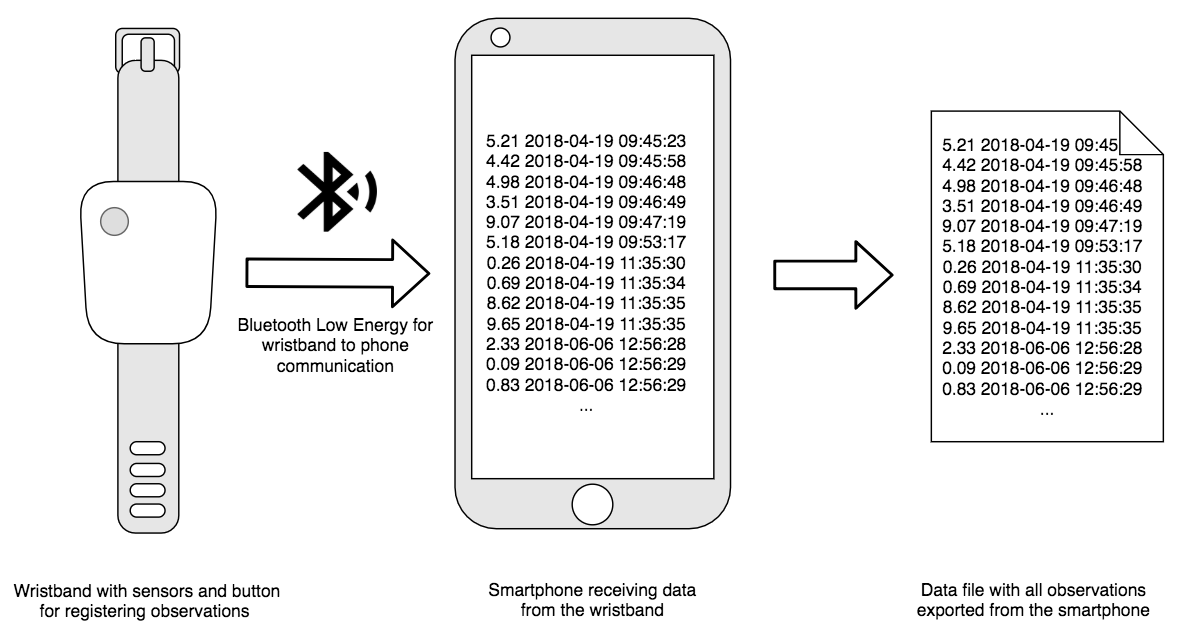
\includegraphics[width=1\textwidth]{figures/design_overview.png}
    \caption{Wristband device with sensors and a button for registering observation. Smartphone to import, display and export the data}
    \label{design_overview}
\end{figure}


\section{Functionalities \& Requirements}\label{requirements}
With the general outline for the wristband and companion app laid out, we can create a list of functionalities and requirements that shall be implemented in order to create a MVP.

\begin{itemize}
    \item \textbf{Log data:} The user should be able to log observation using the wristband, this should be possible to do independently from the companion app
    \item \textbf{Import data:} The companion app shall import the logged data from the wristband
    \item \textbf{Display data:} The companion app shall display the logged data (scaled value and time stamp)
    \item \textbf{Export data:} The companion app shall be able to export the logged data to a data file for further investigation
	\item \textbf{Simple solution:} It should be simple and easy to perform all of the above actions.
\end{itemize}
\chapter{Implementation}\label{implementation}\label{implem_ch}

TODO: Chapter introduction

\textbf{COMMENT: Perhaps upfront explain the process with the prototypes?}

\section{Proof of Concept}
Before the actual implementation of the design from the previous Chapter, a Proof of Concept (PoC) was created. This had several purposed, first to see if it was at all possible to have at least some sense of the scale when performing the gestures, secondly \textbf{?? what are other good reasons?}. The component listed bellow was connected together as shown in Figure \ref{sketch_bb} and \ref{sketch_schem}, the finished PoC can be seen in Figure \ref{poc}.

\begin{itemize}
    \item Adafruit Feather M0 Adalogger\cite{adalogger} with a 340mAh 3.7V battery
    \item Adafruit 9-DOF Absolute Orientation IMU Fusion Breakout - BNO055\cite{gyro}
	\item Flora Wearable Bluefruit LE Module\cite{bluefruit}
	\item A push button
	\item A 100k$\Omega$ resistor
\end{itemize}

The Feather M0 Adalogger was controlled by an Arduino script, that after establishing a bluetooth connection waits for the button to be pressed. When the button is pressed the Euler angles from the IMU is read, and transmitted over the bluetooth connection, the LED is connected to the switch so it will light up as long as the button is pressed. A simple GUI (as seen in Figure \ref{poc_s1}) was created using a Python script, that connected to the bluetooth module and when receiving data displayed the raw values and the mapped scaled value between zero and ten. Both the Arduino and Python scrips are linked to in Appendix \ref{poc_code}.

\begin{figure}[h!]
    \centering
    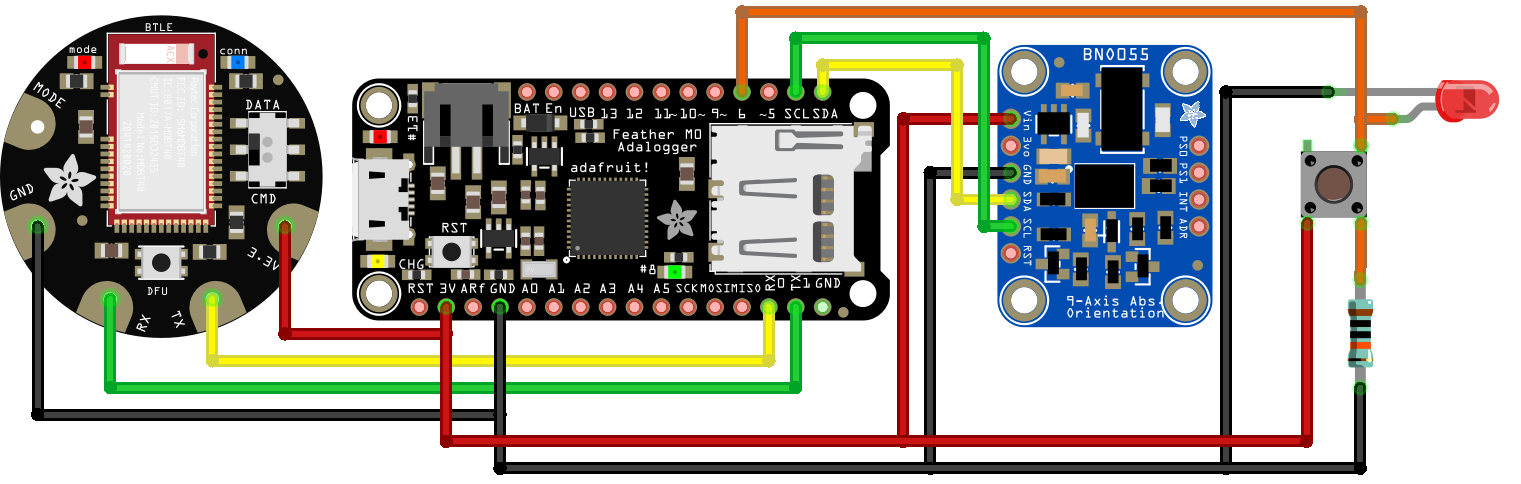
\includegraphics[width=1\textwidth]{figures/Sketch_bb.png}
    \caption{Wiring for of the proof of concept. Battery not shown}
    \label{sketch_bb}
\end{figure}

\begin{figure}[h!]
    \centering
    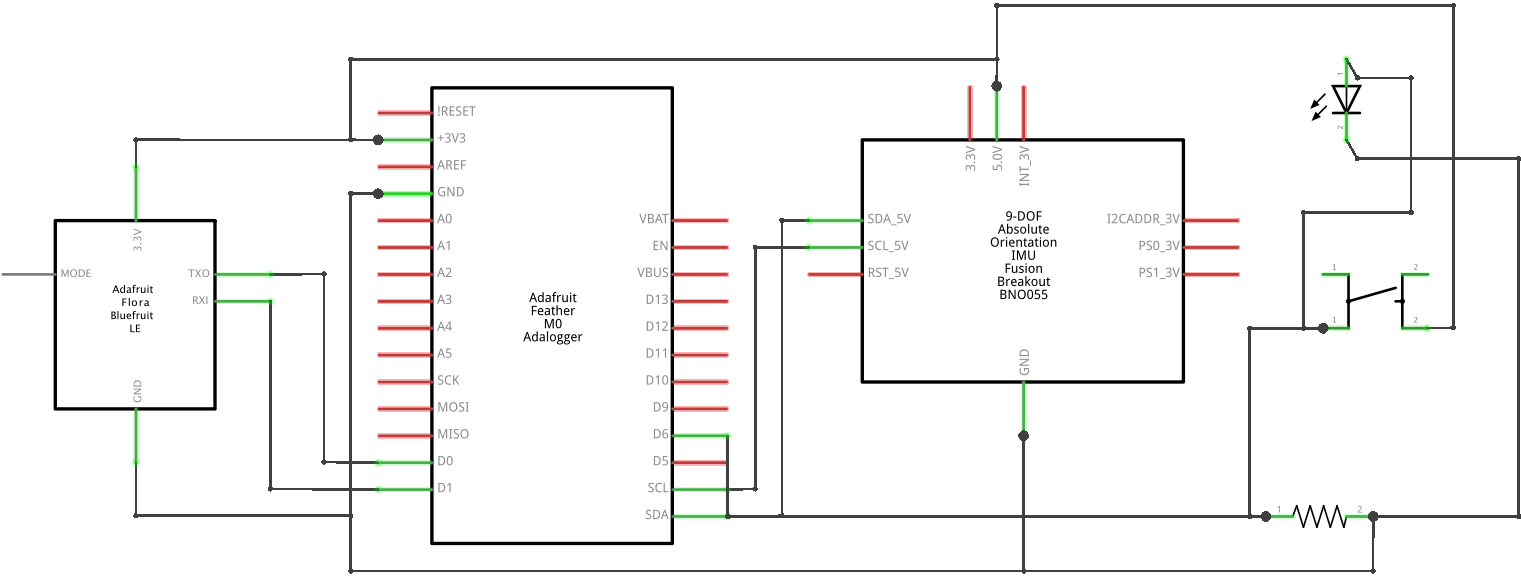
\includegraphics[width=1\textwidth]{figures/Sketch_schem.png}
    \caption{Schematic for the proof of concept. Battery not shown}
    \label{sketch_schem}
\end{figure}

\begin{figure}[h!]
    \centering
    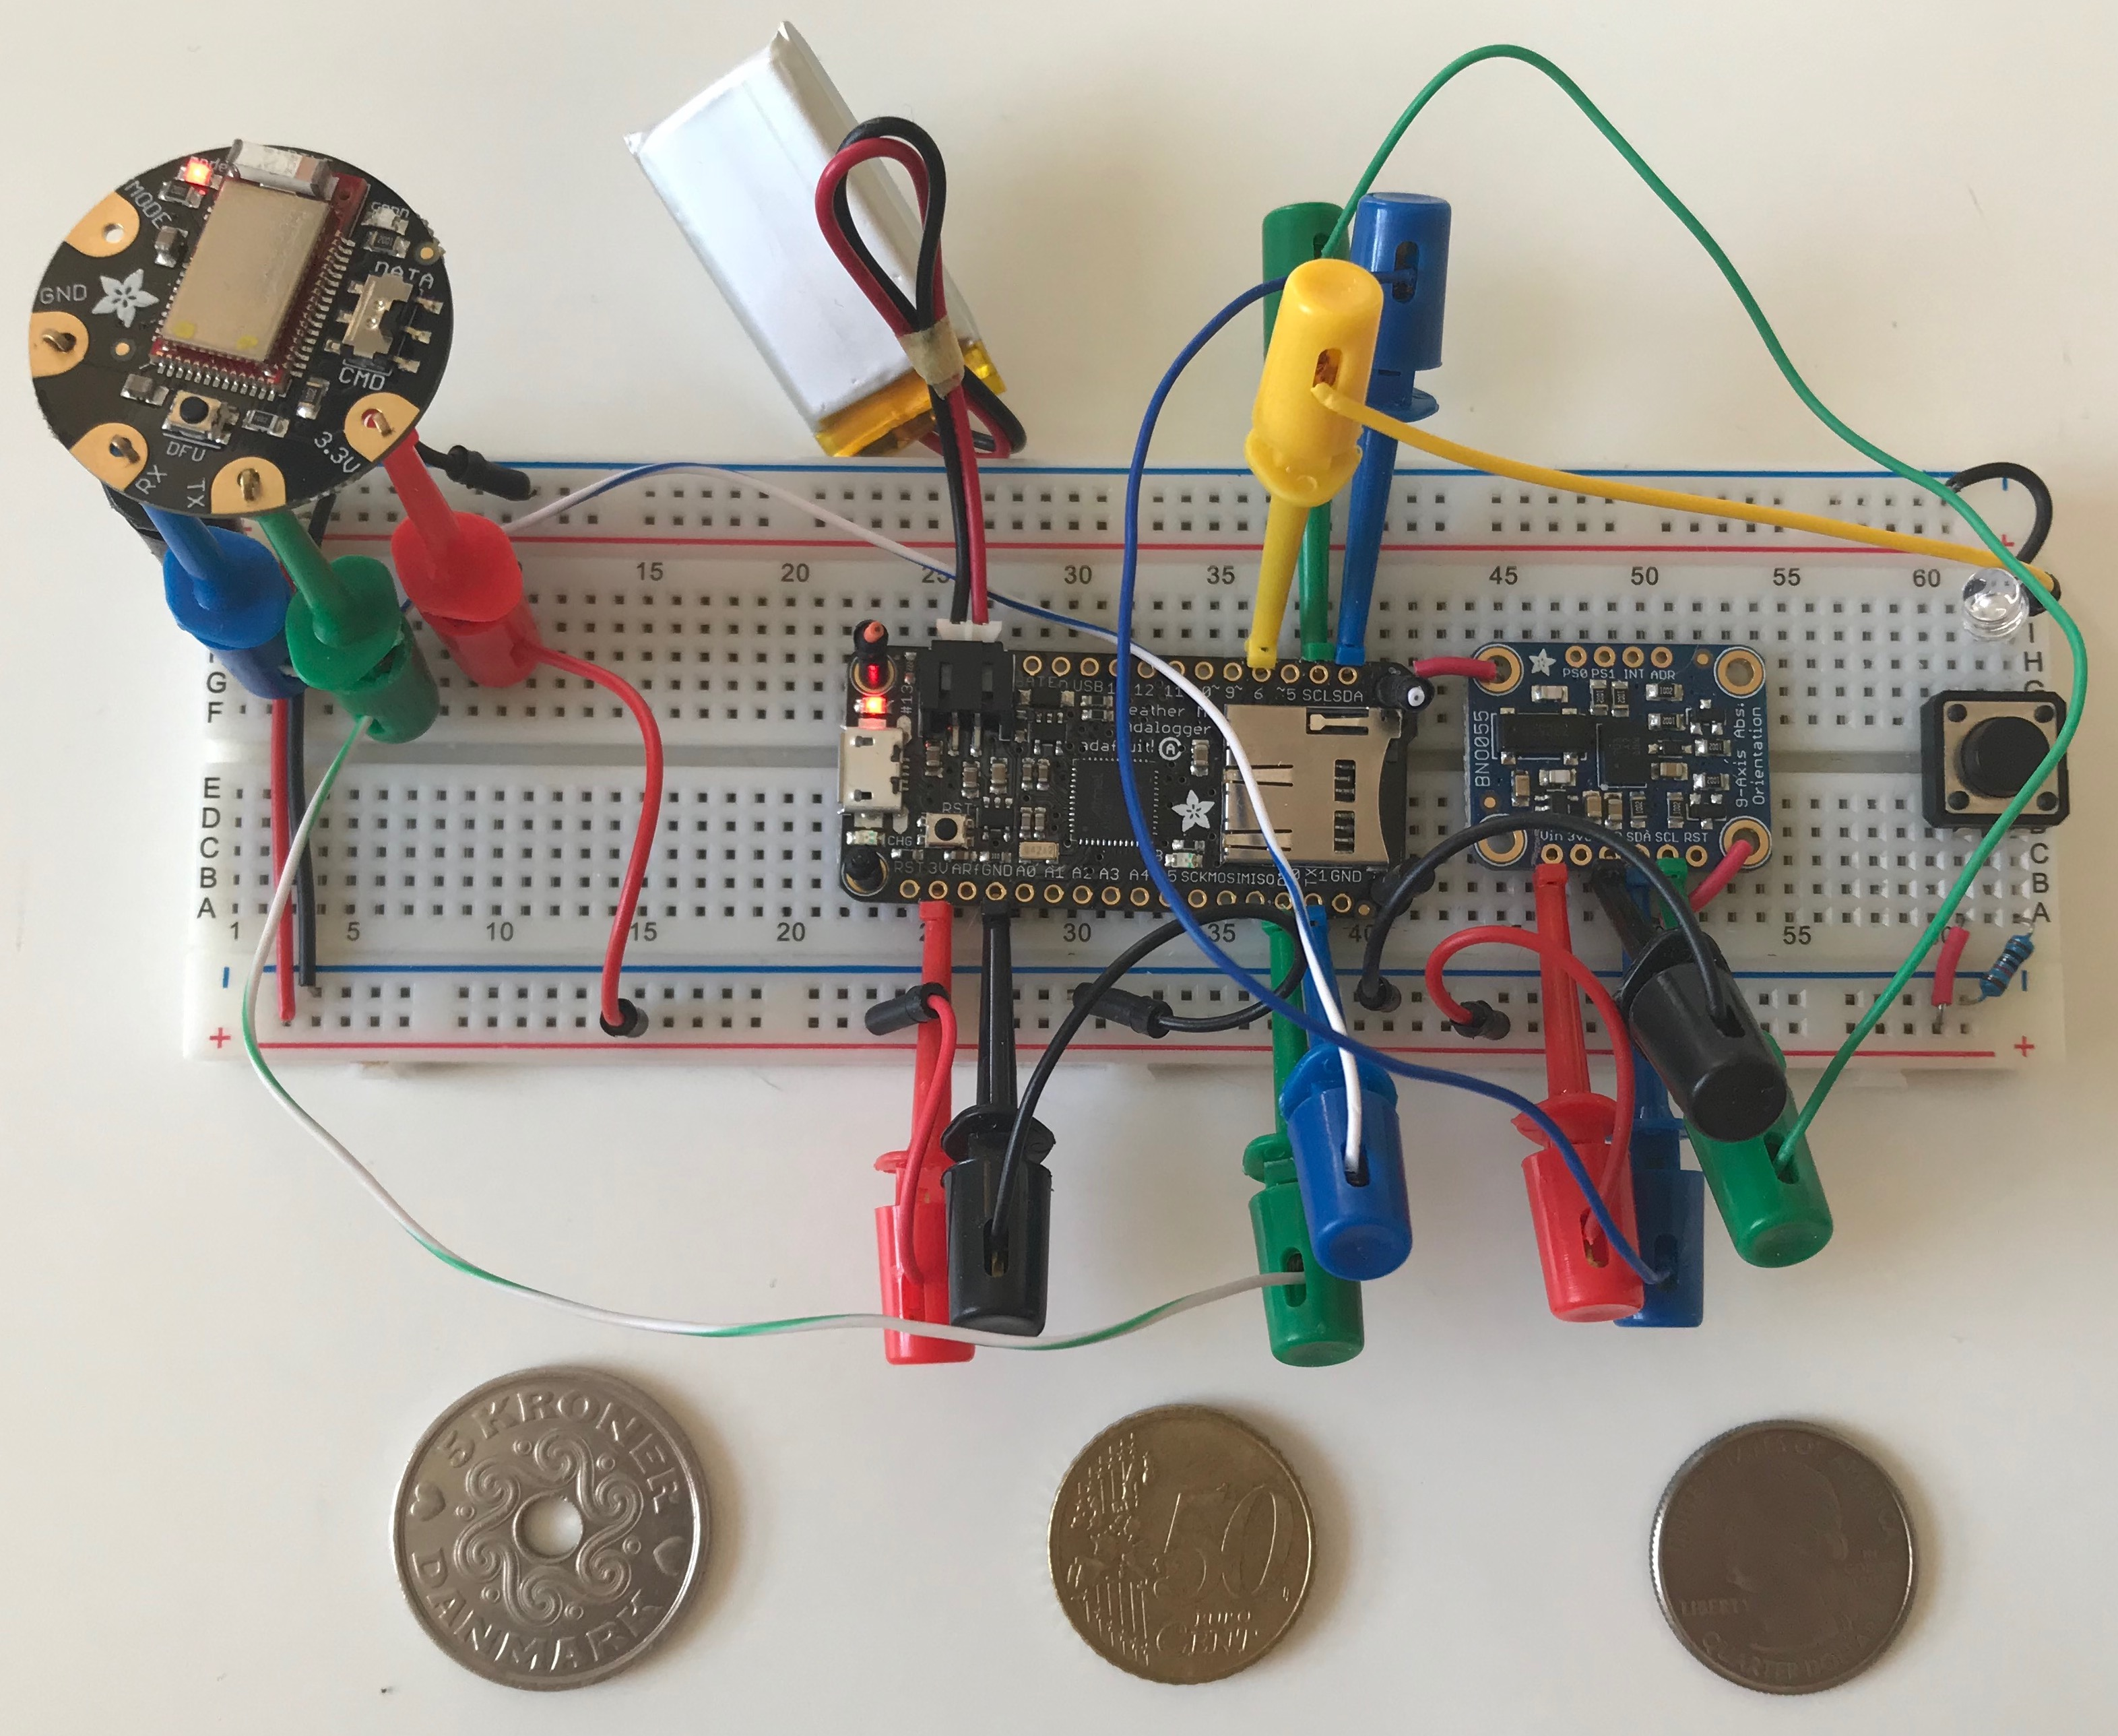
\includegraphics[width=0.6\textwidth]{figures/poc.jpg}
    \caption{Proof of concept. Components from left to right on the breadboard: Bluefruit LE Module, Feather M0 Adalogger and battery, IMU Fusion Breakout - BNO055, push button and led. Coins below for scale (5dkk, 0.5\EURtm{} \& 0.25\$)}
    \label{poc}
\end{figure}

The PoC was tested by strapping it to the back of the lower arm using rubber bands, then moving the arm to different positions within the gestures described earlier and pressing the button. It was validated that the concept worked, and it was possible to input different values using the gesture. The question still remained how precise it was. At this point the author thought that this concept would only be precise enough to be used on a three point scale and would not be able to compete with a VAS.

\begin{figure}[h!]
    \centering
    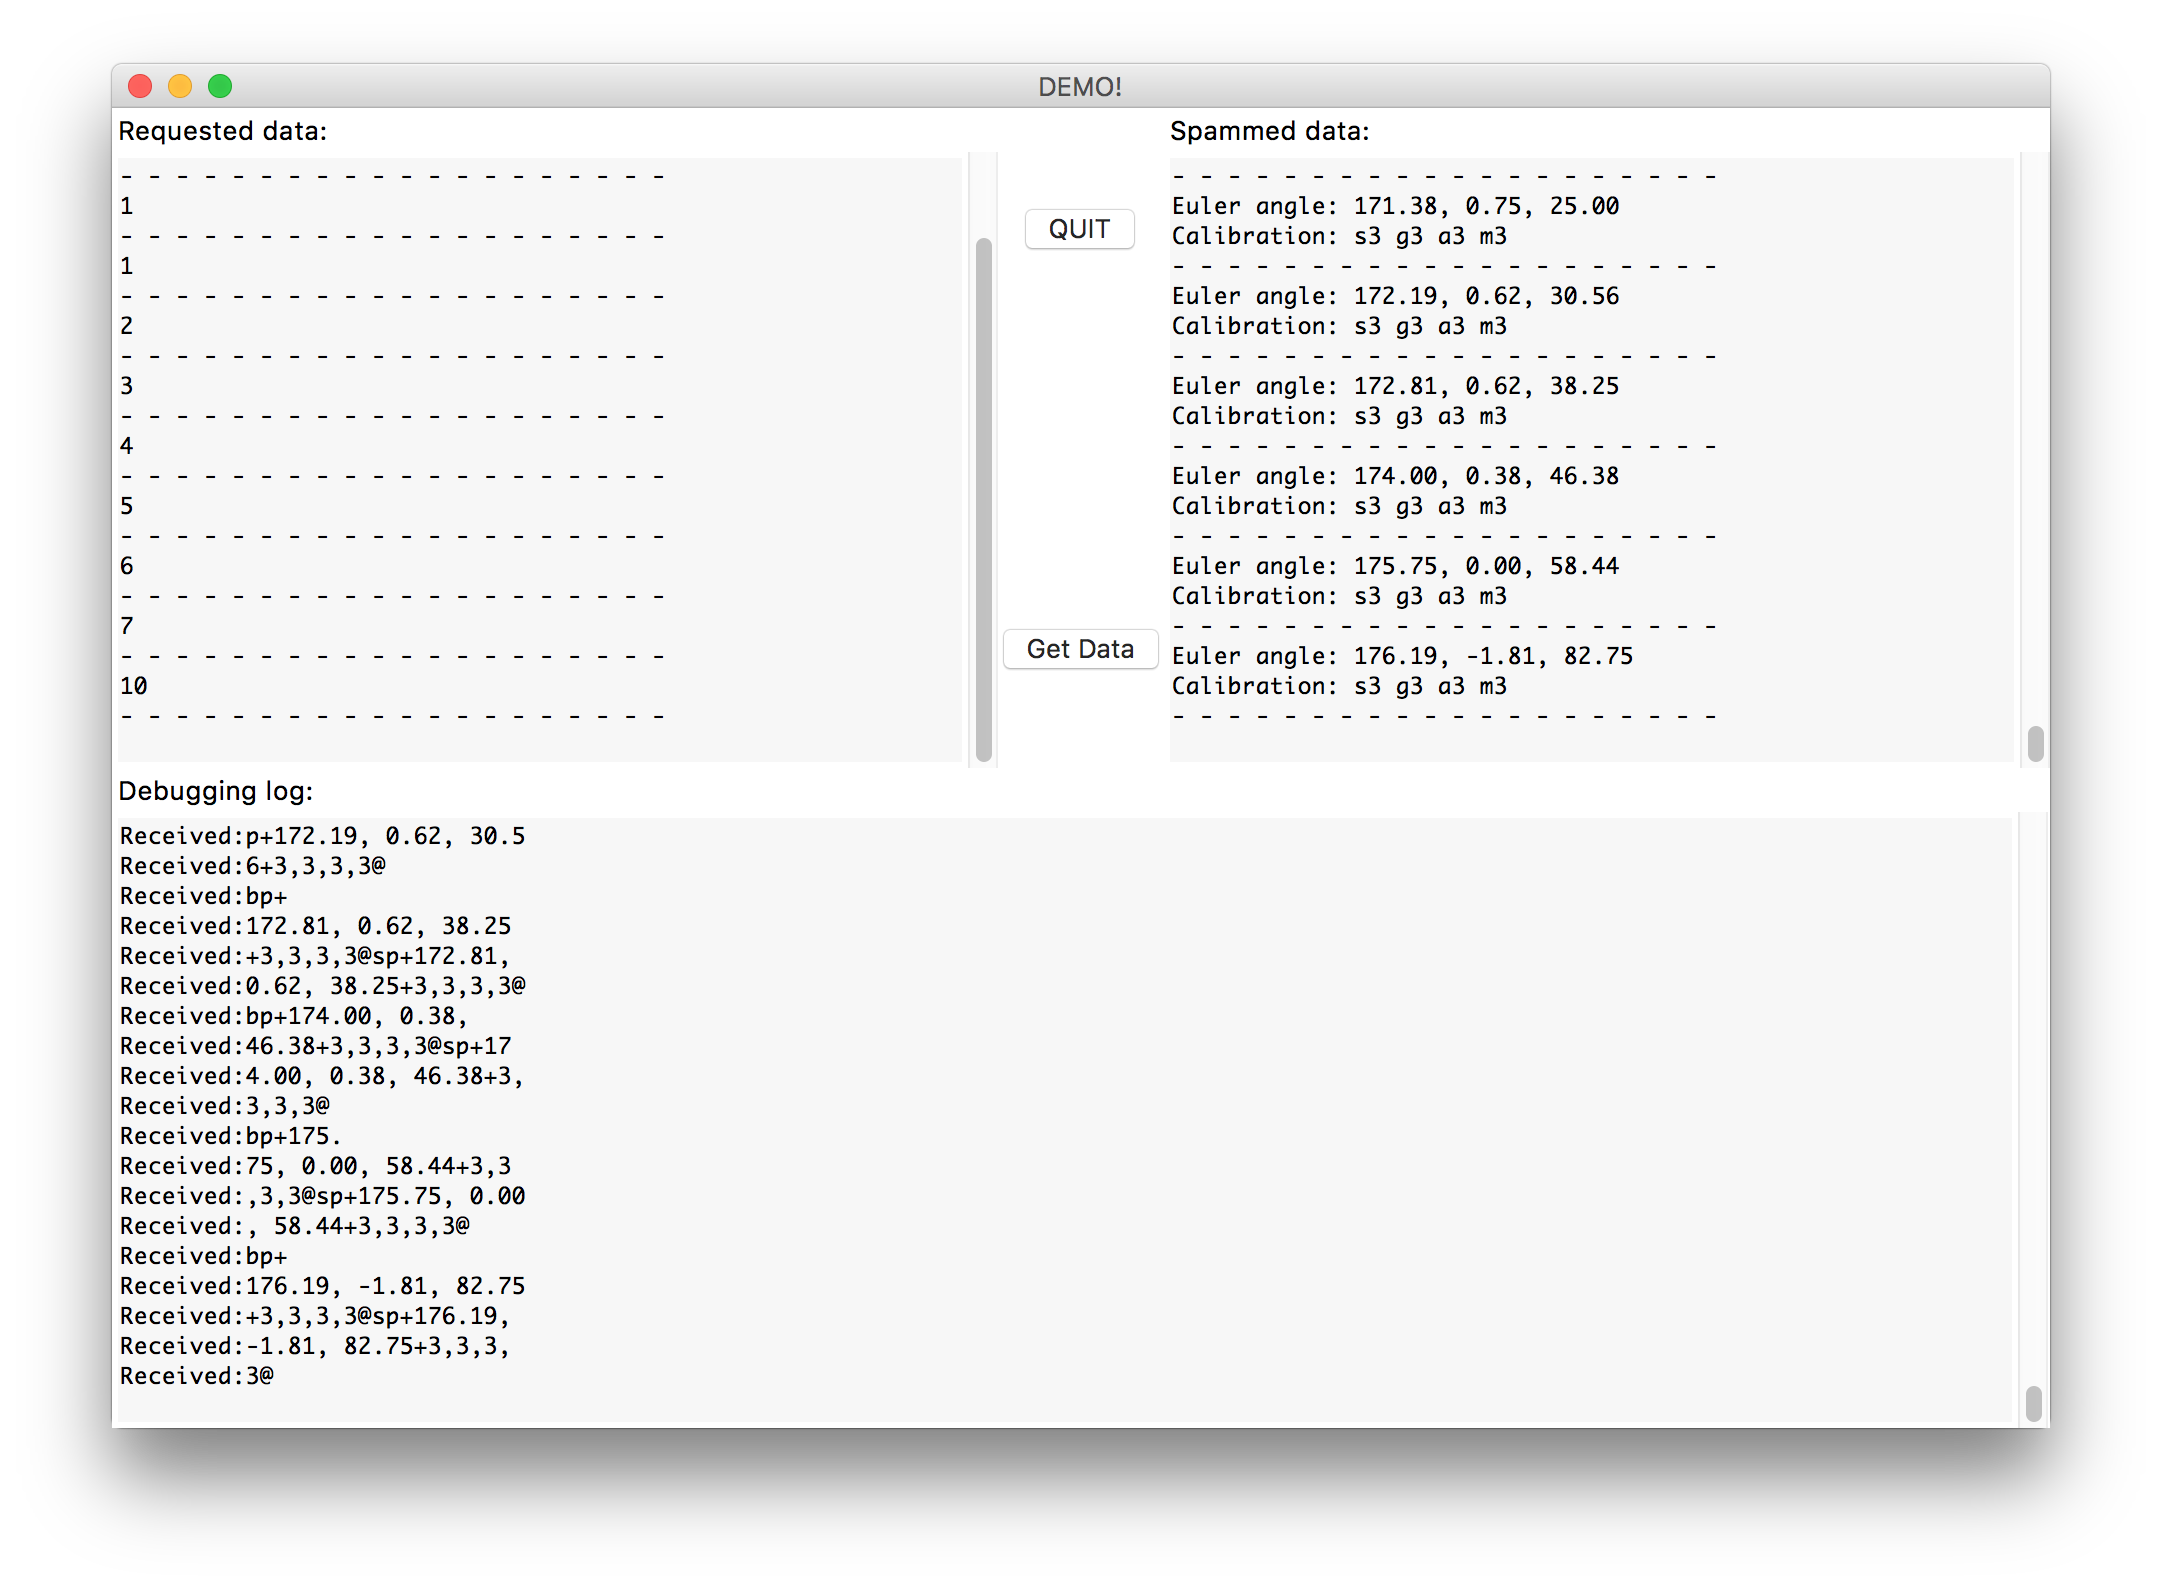
\includegraphics[width=1.2\textwidth]{figures/poc_s1.png}
    \caption{PoC GUI. Top left shows the data mapped to the 0-10 scale. Top right shows the raw data and calibration. Bottom shows a debug log}
    \label{poc_s1}
\end{figure}


\section{Prototype}
With the PoC being a success the design from Chapter \ref{design_ch} could be implemented. The components used for the PoC could in theory be rearranged and soldered together into a more compact design, but in practice it would be quite bulky for a wristband device. Instead a small device called \say{MetaMotionR} created by mbientlab\cite{mbient} was used. The device is roughly the same size as a regular wrist watch, although thicker, and is packed with sensors, most importantly an IMU with the same Sensor Fusion algorithm as the BNO055. The MetaMotionR is also equipped with a push button and has Low Energy Bluetooth built in, making it an excellent hardware choice for this implementation.

\begin{figure}[h!]
    \centering
    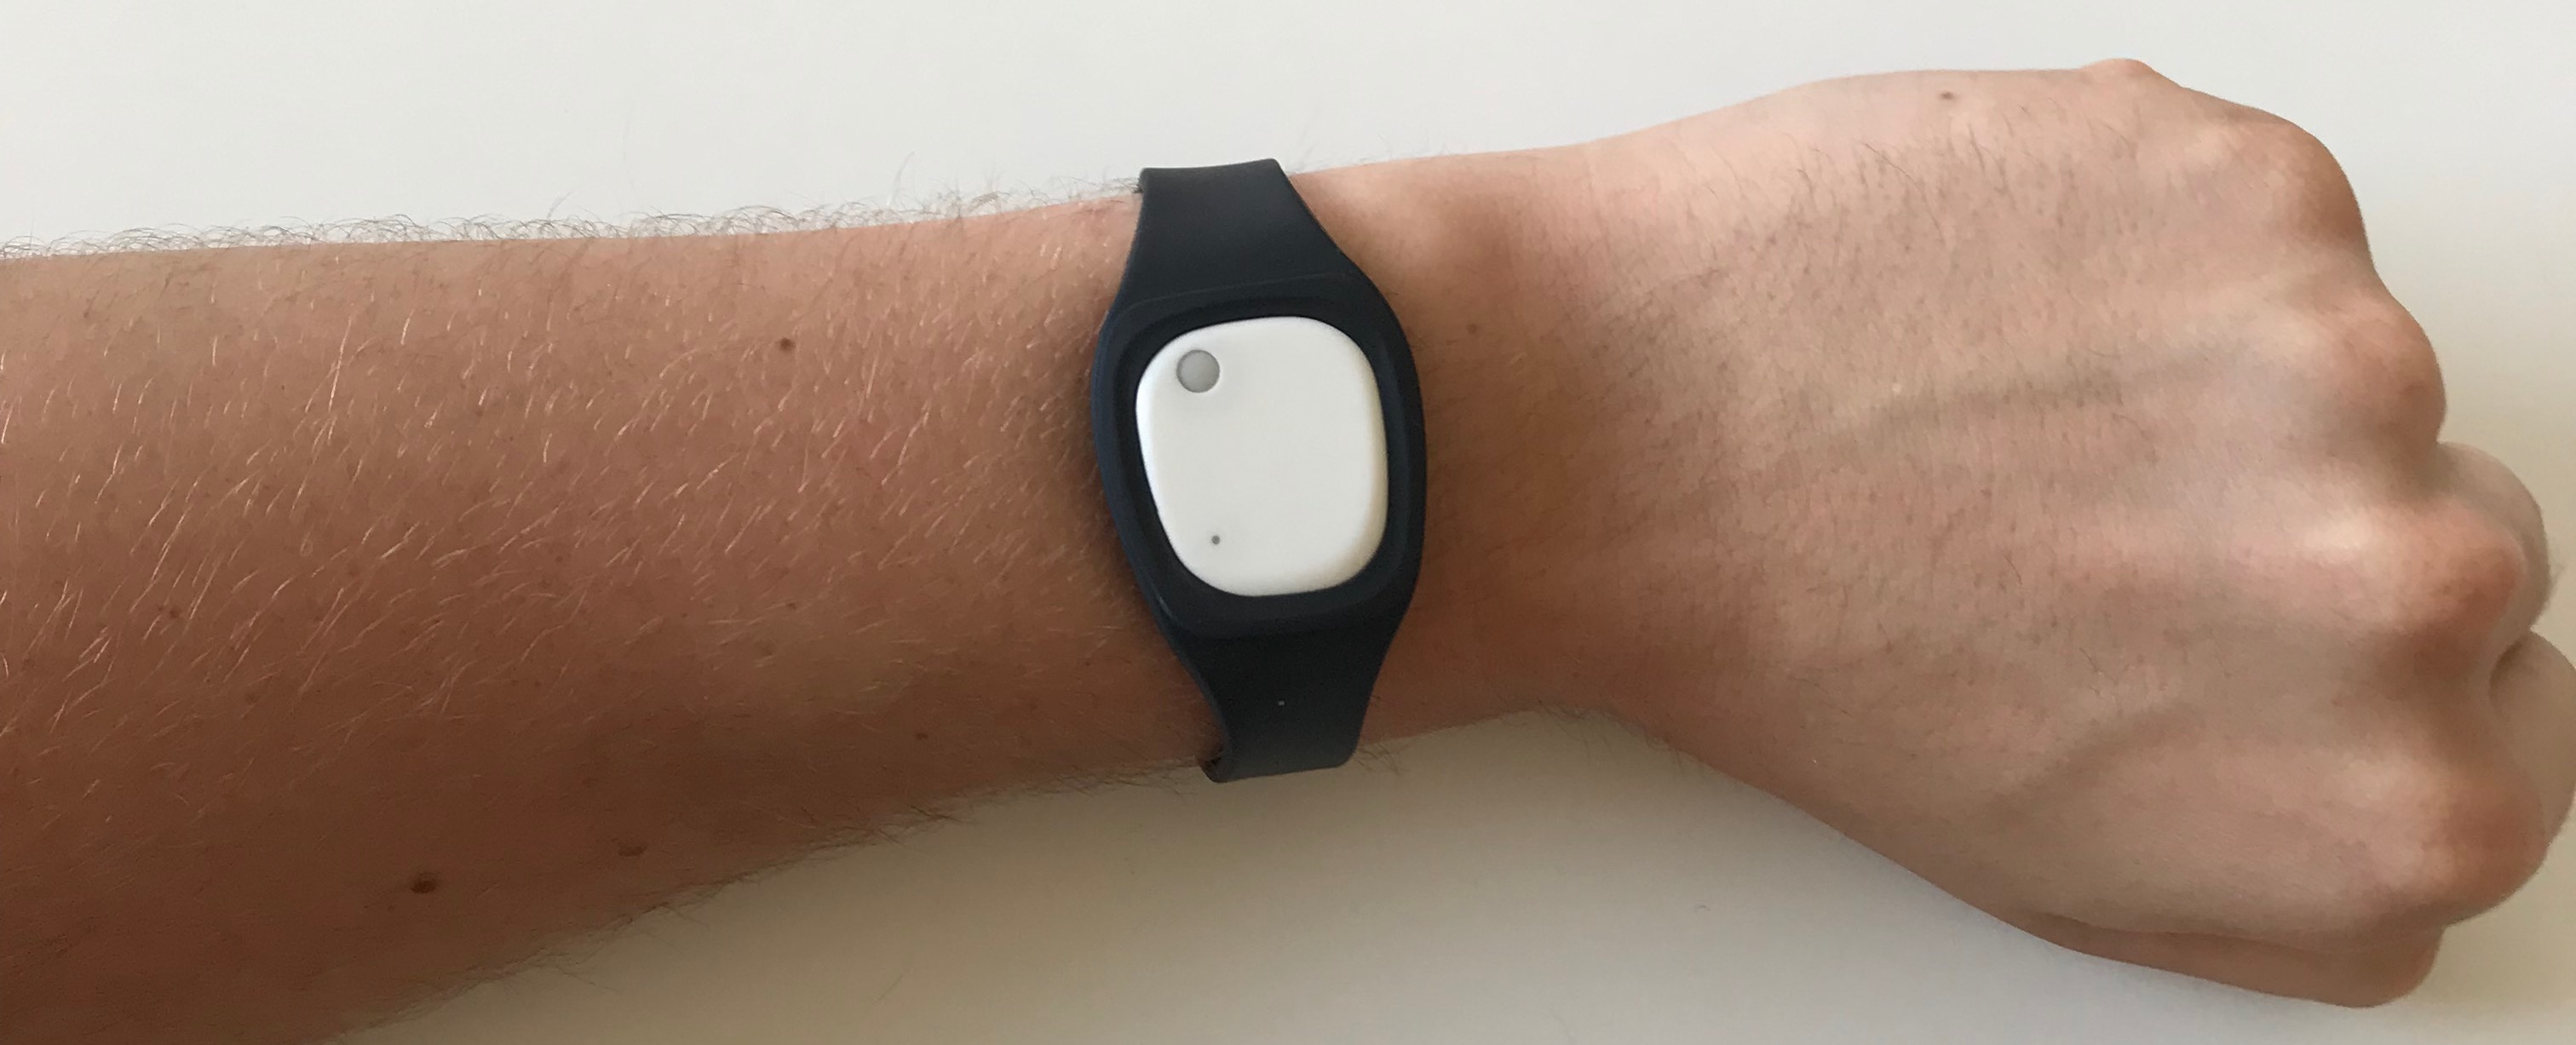
\includegraphics[width=0.6\textwidth]{figures/mbient.jpg}
    \caption{MetaMotionR by mbientlab\cite{mbient}}
    \label{mbient}
\end{figure}

The MetaMotionR must be programmed using mbientlab's API, available for several platforms\cite{api_mbient}. Since the design all ready requires a companion app for the wristband the API for Android will be used. The MetaMotionR has 8MB of flash memory which can be used to store commands and log data, it allows for more than 200.000 log entries when logging Euler angles, which should be more than enough for this use case. The MetaMotionR is programmed to run the Sensor Fusion algorithm and whenever the button us pressed it will log the current orientation, turn its LED on and vibrate to give user feedback. It was considered to use the vibration motor to give varied feedback dependent on the value logged, but the vibration motor doesn't offer much customization, only the time interval can be customized, and if the vibration is any shorter than half a second it might not vibrate, therefor this idea was discarded for this implementation.

When the companion app connects to the MetaMotionR the logged data can be imported over the app and is afterwards deleted from the MetaMotionR to free up space for future data entries. Beside storing the Euler angles each data entry has a time stamp. The time on the MetaMotionR is synchronized whenever it connects to a smartphone. One flaw with the MetaMotionR is that logged entries and the commands are stored in the flash memory, which requires power, this means that if the MetaMotionR runs of power all logged entries will be lost, and it needs to connect to the companion app before it can be used to log entries again. The battery life of the MetaMotionR will be explored later in this Chapter. 

\section{Android App}
Following the requirements from Section \ref{requirements} the companion was implemented. The app was build upon mbientlab's tutorial \say{starter app}\cite{starter_mbient}. The starter app handles the bluetooth connectivity (searching for devices and connected), beside this the rest was left to be implemented. As explained the app programs the MetaMotionR, this happens every time the device connects to the app. The app consist of three buttons, one to import, share and delete data. The largest part of the screen is reserved for displaying the data in a scroolable list, with the latest entry on top. When the data is imported from the device the Euler angles get mapped to the scaled value, this value together with the Euler angles, time stamps and battery percentage of the MetaMotionR are saved to internal file (in CSV format). The scaled values are displayed in the app together with its time stamp and battery percentage. After data has been imported it is deleted from the MetaMotionR. The \say{Delete Data} button lets the user delete the data that has been imported to the app, when pressed a confirmation dialogue appears to prevent accidental deletion. If confirmed the app will delete the internal file containing the data. The \say{Share Data} button lets the user export the data via. email. When pressed the app creates a copy of the internal file to external storage, an intent is then made to create an email with the file attached. The email can then be send and the attached data can be examined in a spreadsheet or other tool. Lastly the app has a toggle switch labeled \say{Time Only}. The default configuration is to have this toggle off, in this state the MetaMotionR behaves as described. If the toggle is on the MetaMotionR is programmed into a \say{Battery Saver} mode, where the Sensor Fusion will be turned off, and therefor Euler angles and scaled values wont be logged. Data entries made in this state will be listed with \say{--} instead of the scaled value. This mode was implemented after it was discovered that the battery life of the MetaMotionR didn't live up to expectaion, more on this later. The finished app can be seen in Figure \ref{proto_s1}. The code used to display, share and delete the data in the companion app was based on the code from the authors previous project \say{Mood Tracker}\cite{mood}.

\begin{figure}[h!]
    \centering
    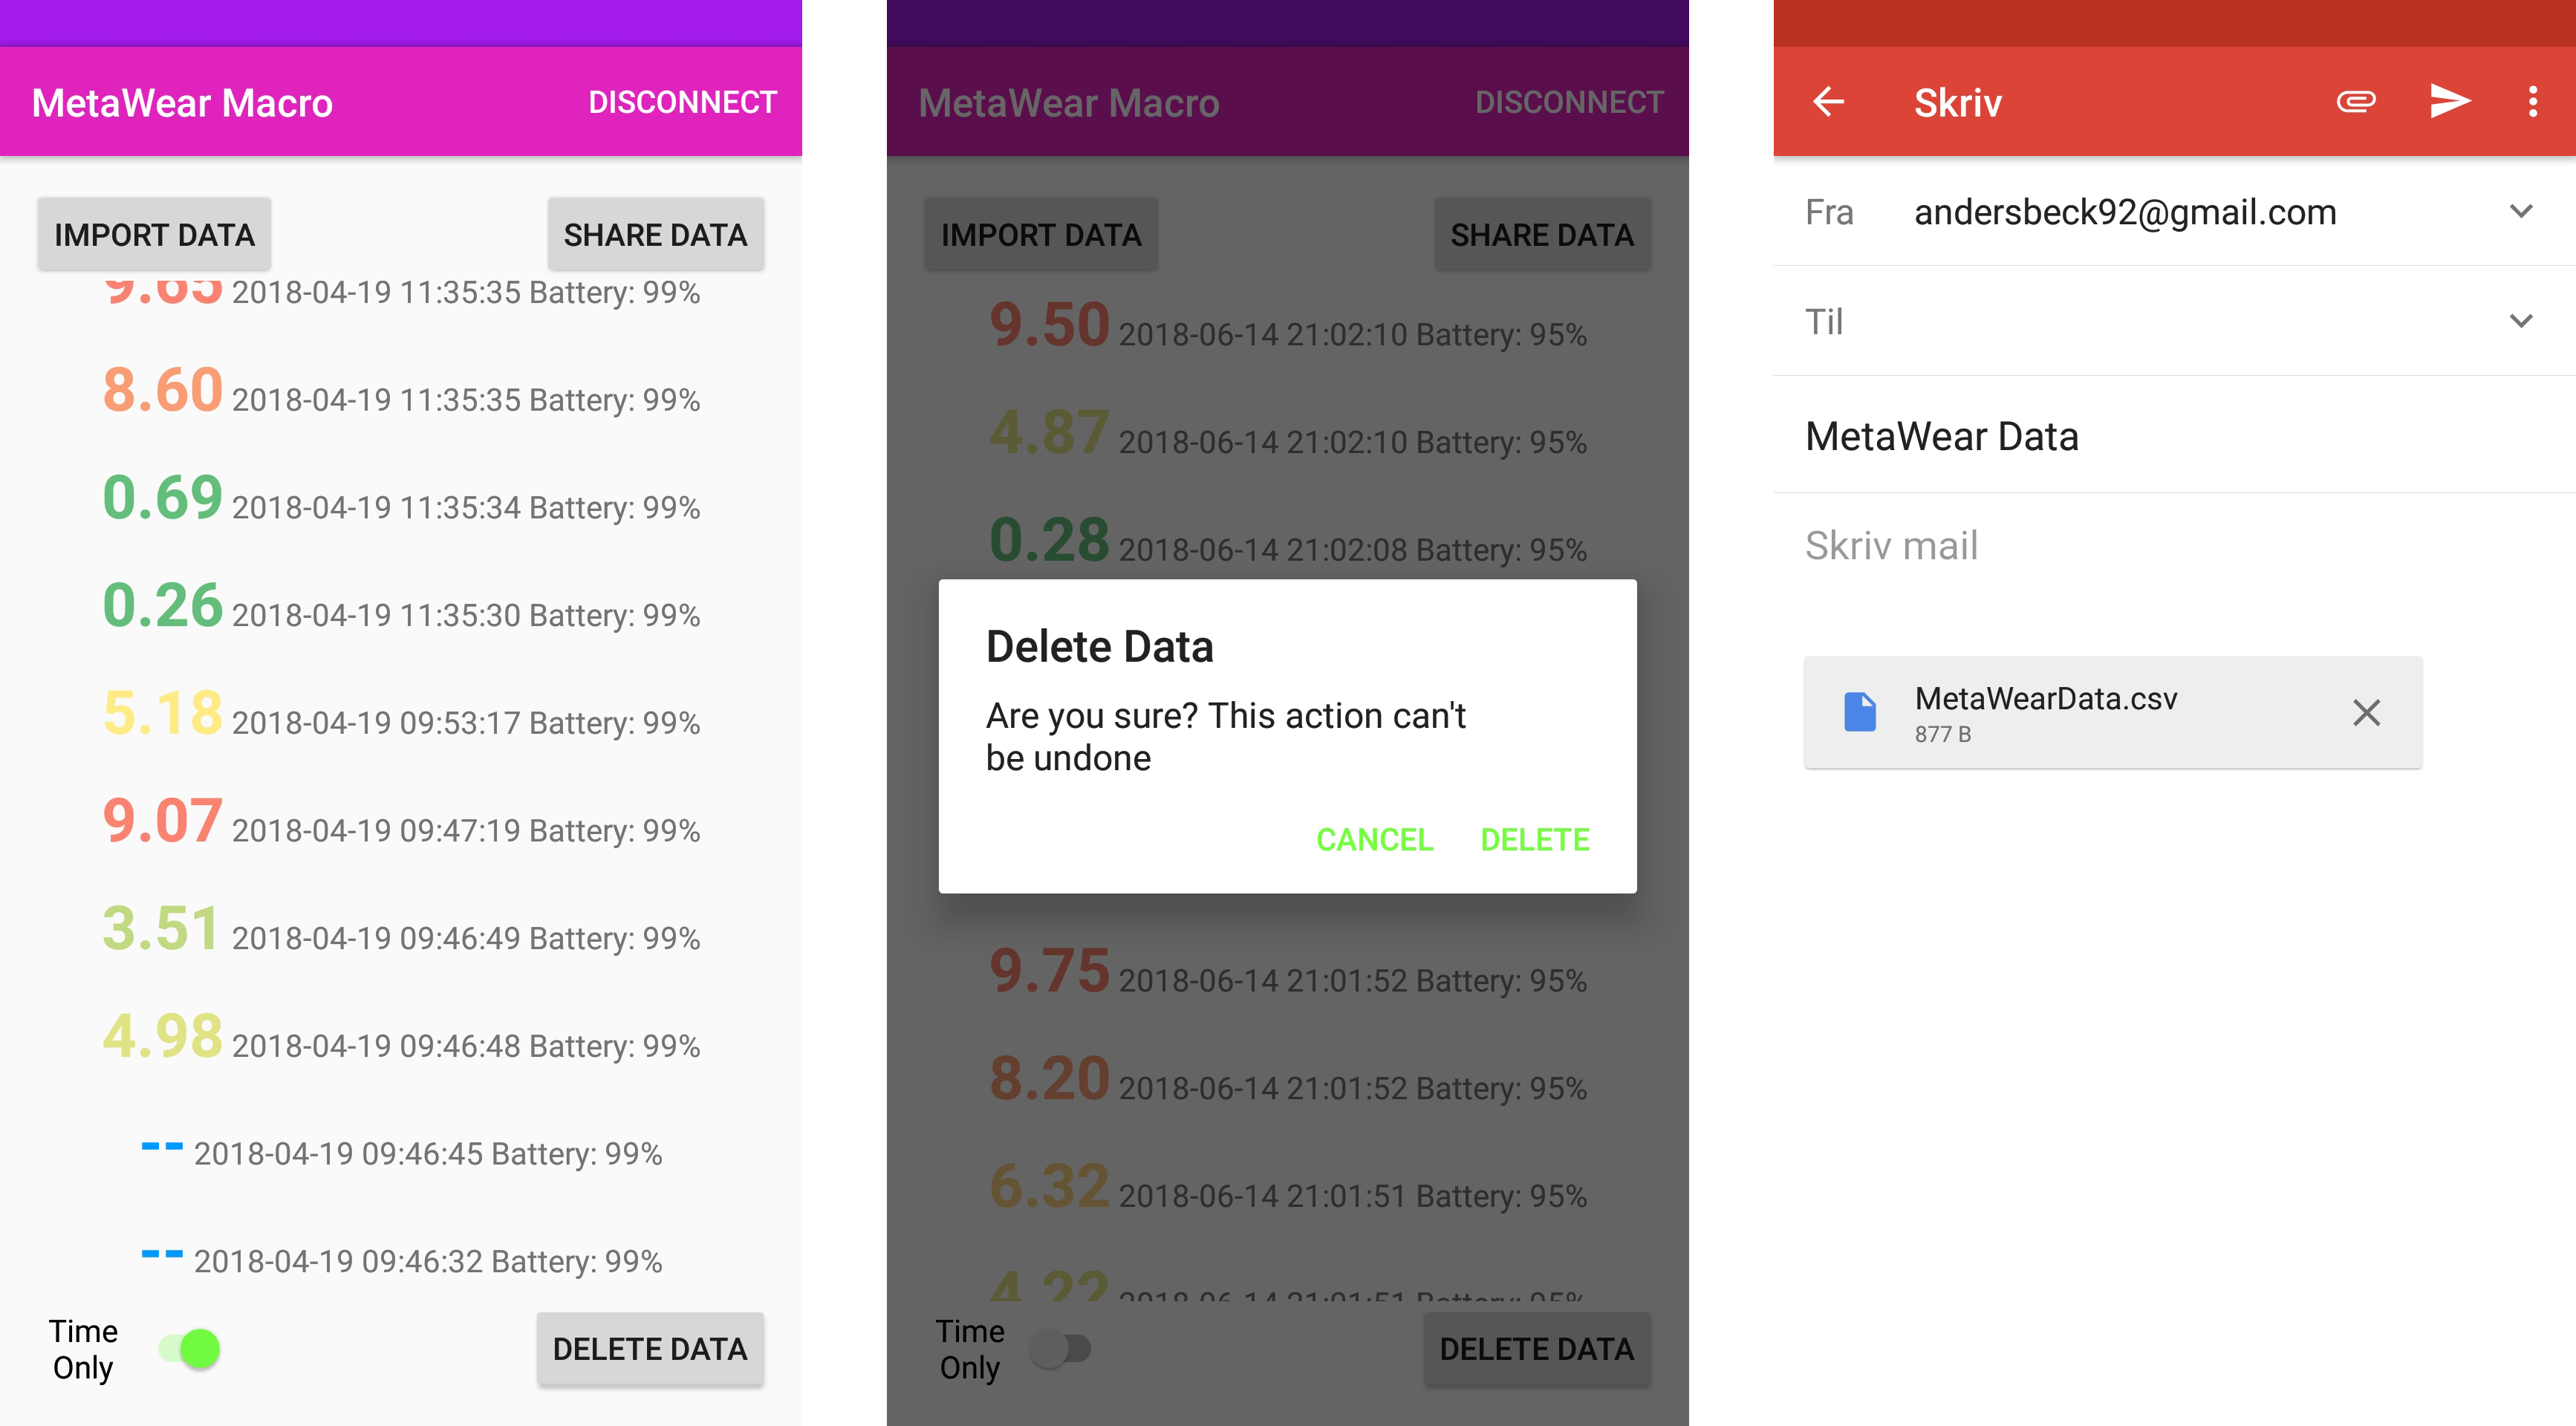
\includegraphics[width=1\textwidth]{figures/proto_s1.png}
    \caption{Companion app. Main screen on the left, Delete Data in the middle \& Share Data on the right}
    \label{proto_s1}
\end{figure}



\section{Testing}
The performance of the MetaMotionR and the companion app was tested throughout the implementation process, this was done to ensure that it worked as intended. In this testing is was discovered that the battery life of the MetaMotionR was quite limited, depended on the workload. A artificial test was setup to simulate a worst case scenario, the MetaMotionR was programmed to read and transmit the Euler angles to the companion app once every second. The battery percentage was noted at about every 15-30 minutes until the MetaMotionR ran out of battery. The test was run twice, and the results can be seen in Figure \ref{battery_test}, the first test ran for a little less than five hours, while the second time only ran for a little over two hours. These results disappointing, but the test were extreme and real usage would not be that demanding. In order to get a feel of what could be expected by the MetaMotionR in real use, the author choose to wear the device every day for one week, logging entries at least 20 times a day at random times. What was found that with this demand the device could run for at least one day without a charge. It was discovered that the battery percentage would stay in the $\thicksim$90-80\% range through most of the day and night, and once the battery percentage came below $\thicksim$70-60\% it would dramatically drop to zero. Because of this, it was decided to implement the option to disable the logging of orientation, so if this device and app were to be used in real life, one could still get the time stamp recorded which is still valuable information to collect as shown by Larsen et al.\cite{eg}. When used in this mode the battery life is much longer, how long is unknown but it was able to hold a comfortable battery percentage for over a week. One benefit to the battery is that it will fully charge in less than 2 minites.

\begin{figure}[h!]
    \centering
    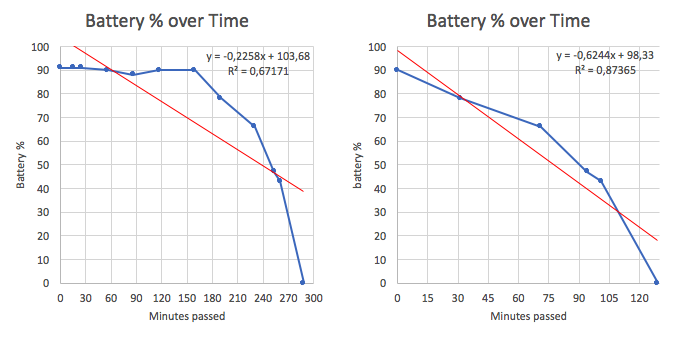
\includegraphics[width=1\textwidth]{figures/batteryTest.png}
    \caption{Battery Tests}
    \label{battery_test}
\end{figure}
\chapter{Experiment}

This chapter will describe the method of the experiment conducted in order to compare the gestures using the wristband to a VAS. For comparison a test was designed where the participants would be shown a stimuli and asked to input it using the gestures or a digital VAS. Two kinds of stimuli was used, an integer between zero and one hundred, or a box with a shade of grey between white and black based on the experiment by Matejka et al.\cite{grey}. Before describing the experiment further lets declare some terms for better clarification. As stated, there are three input methods:

\begin{enumerate}
\item The digital VAS. This is using a slider on the tablet. This input method will be referred to as \say{slider}
\item Using the wristband and the gesture of turning the wrist as described in Figure \ref{roll}. This input method will be referred to as \say{wrist}
\item Using the wristband and the gesture of raising the lower arm as described in Figure \ref{pitch}. This input method will be referred to as \say{arm}
\end{enumerate}

The two types of stimuli will be referred to as \say{num} and \say{grey} for the integer and shade of grey respectfully. With these three input methods and two stimuli a total of six different exercises must be conducted. The naming for each of these exercises is a combination of the input method and stimuli, e.g. turning your wrist to input a shade of grey will be referred to as \say{wrist\_grey}. All of the exercise's names can be seen in the top of Table \ref{latin}. The rest of this section will cover every aspect of this in more detail.

% % % % % % % % % % % % % % % % % % % % % % % %
% Participants % Participants % Participants %
% % % % % % % % % % % % % % % % % % % % % % % %
\section{Participants}
Twenty four (24) participants where chosen for this experiment. Since the experiment consist of six exercises a multiple of six was needed to ensure a minimal bias as explained later. Then based on the time frame for the experiment twenty four seemed to be a reasonable amount while being large enough to collect enough data. The participants volunteered their time and where not paid or in other ways obligated to participate. All of the participants were either from The Department of Applied Mathematics and Computer Science at DTU or the authors colleagues at IBM, thus most of the participants had above average technical experience, but based on the survey conducted after the experiment (Appendix \ref{survey}) 42\% had not any prior experience with wearable devices.

Out of the twenty four participants 18 where men and 6 where female. The mean age was 27.83 and the median age was 26.5, both age and gender distribution can be seen in Figure \ref{age_gender}.

\begin{figure}[h!]
    \centering
    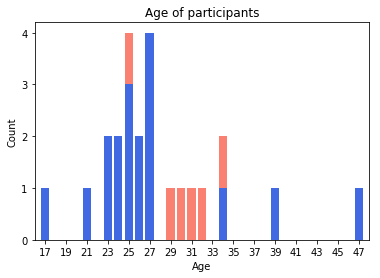
\includegraphics[width=.6\textwidth]{figures/age_gender.png}
    \caption{Age and gender distribution of the 24 participants: 18 males in blue \& 6 females in red}
    \label{age_gender}
\end{figure}



% % % % % % % % % % % % % % % % % % %
% Apparatus % Apparatus % Apparatus %
% % % % % % % % % % % % % % % % % % %
\section{Apparatus}
\subsection{Essential Hardware}
For the experiment three pieces of hardware was used:
\begin{enumerate}
\item MetaMotionR by mbientlab\cite{mbient} as the wristband device for registering input from the participant using the gestures
\item Samsung Galaxy Tab S2\cite{samsung}, this tablet run the app developed for the experimenting, keeping track of exercises, showing stimuli, collecting input from the participant, saving the data etc. Much more detail about this is this section
\item A computer used to fill in the survey after the experiment. In the experiment a MacBook Pro 13 inch model was used, although the computer used isn't important
\end{enumerate}

\subsection{App}
The app created for the experiment is built upon the same code as the companion app described in Chapter \ref{implementation}, but changed to fit the experiment. Has three main functions: Settings, Train and Experiment as seen in Figure \ref{app_main}. The settings is for configuring the experiment and exporting or deleting the collected data as seen in Figure \ref{app_settings}. Two variables can be changed that has influence on the experiment, the first is the \say{Number of stimuli}, this value will change the number of stimuli the participant has to rate for each exercise, the number of stimuli can be changed in steps of five. The \say{Next Subject ID} will change the ID used to identify each subject in the data. The order of exercises for the participant is bases on this value. Both of these settings should not be changed though out the experiment, so that the participant's IDs will be in sequential order and that they have the same amount of stimuli for each exercise. For this experiment the number of stimuli was set two 20 based on pilots tests.

Beside these two settings there is the option to \say{Toggle back button}, when this option is enabled a \say{Back} button will appear on any screen in the app, and when pressed will go back to the main screen. This option is purely for debugging allowing one two go back to the main screen at any point, during the experiment this options should be disabled. 

The last actions on this screen is to export and delete data. There are two options to export the date: \say{Move data} and \say{Email data}, the first will simply copy the collected data from the internal storage of the app to the external storage on the tablet so it can be accessed by any file manager. The later will also copy the date to external storage, but it will create an intent to email the data which will start the default email app and attach the data. \say{Delete data} will delete the collected data from internal storage, a confirmation prompt will appear first to prevent accidental deletion. Whenever the main or setting screen is accessed, the current battery percentage from the MetaMotionR is displayed on the screen, keeping an eye on this prevent the wristband to run out of power in the middle of the experiment.

\begin{figure}[h!]
\centering
\begin{minipage}{.55\textwidth}
  \centering
  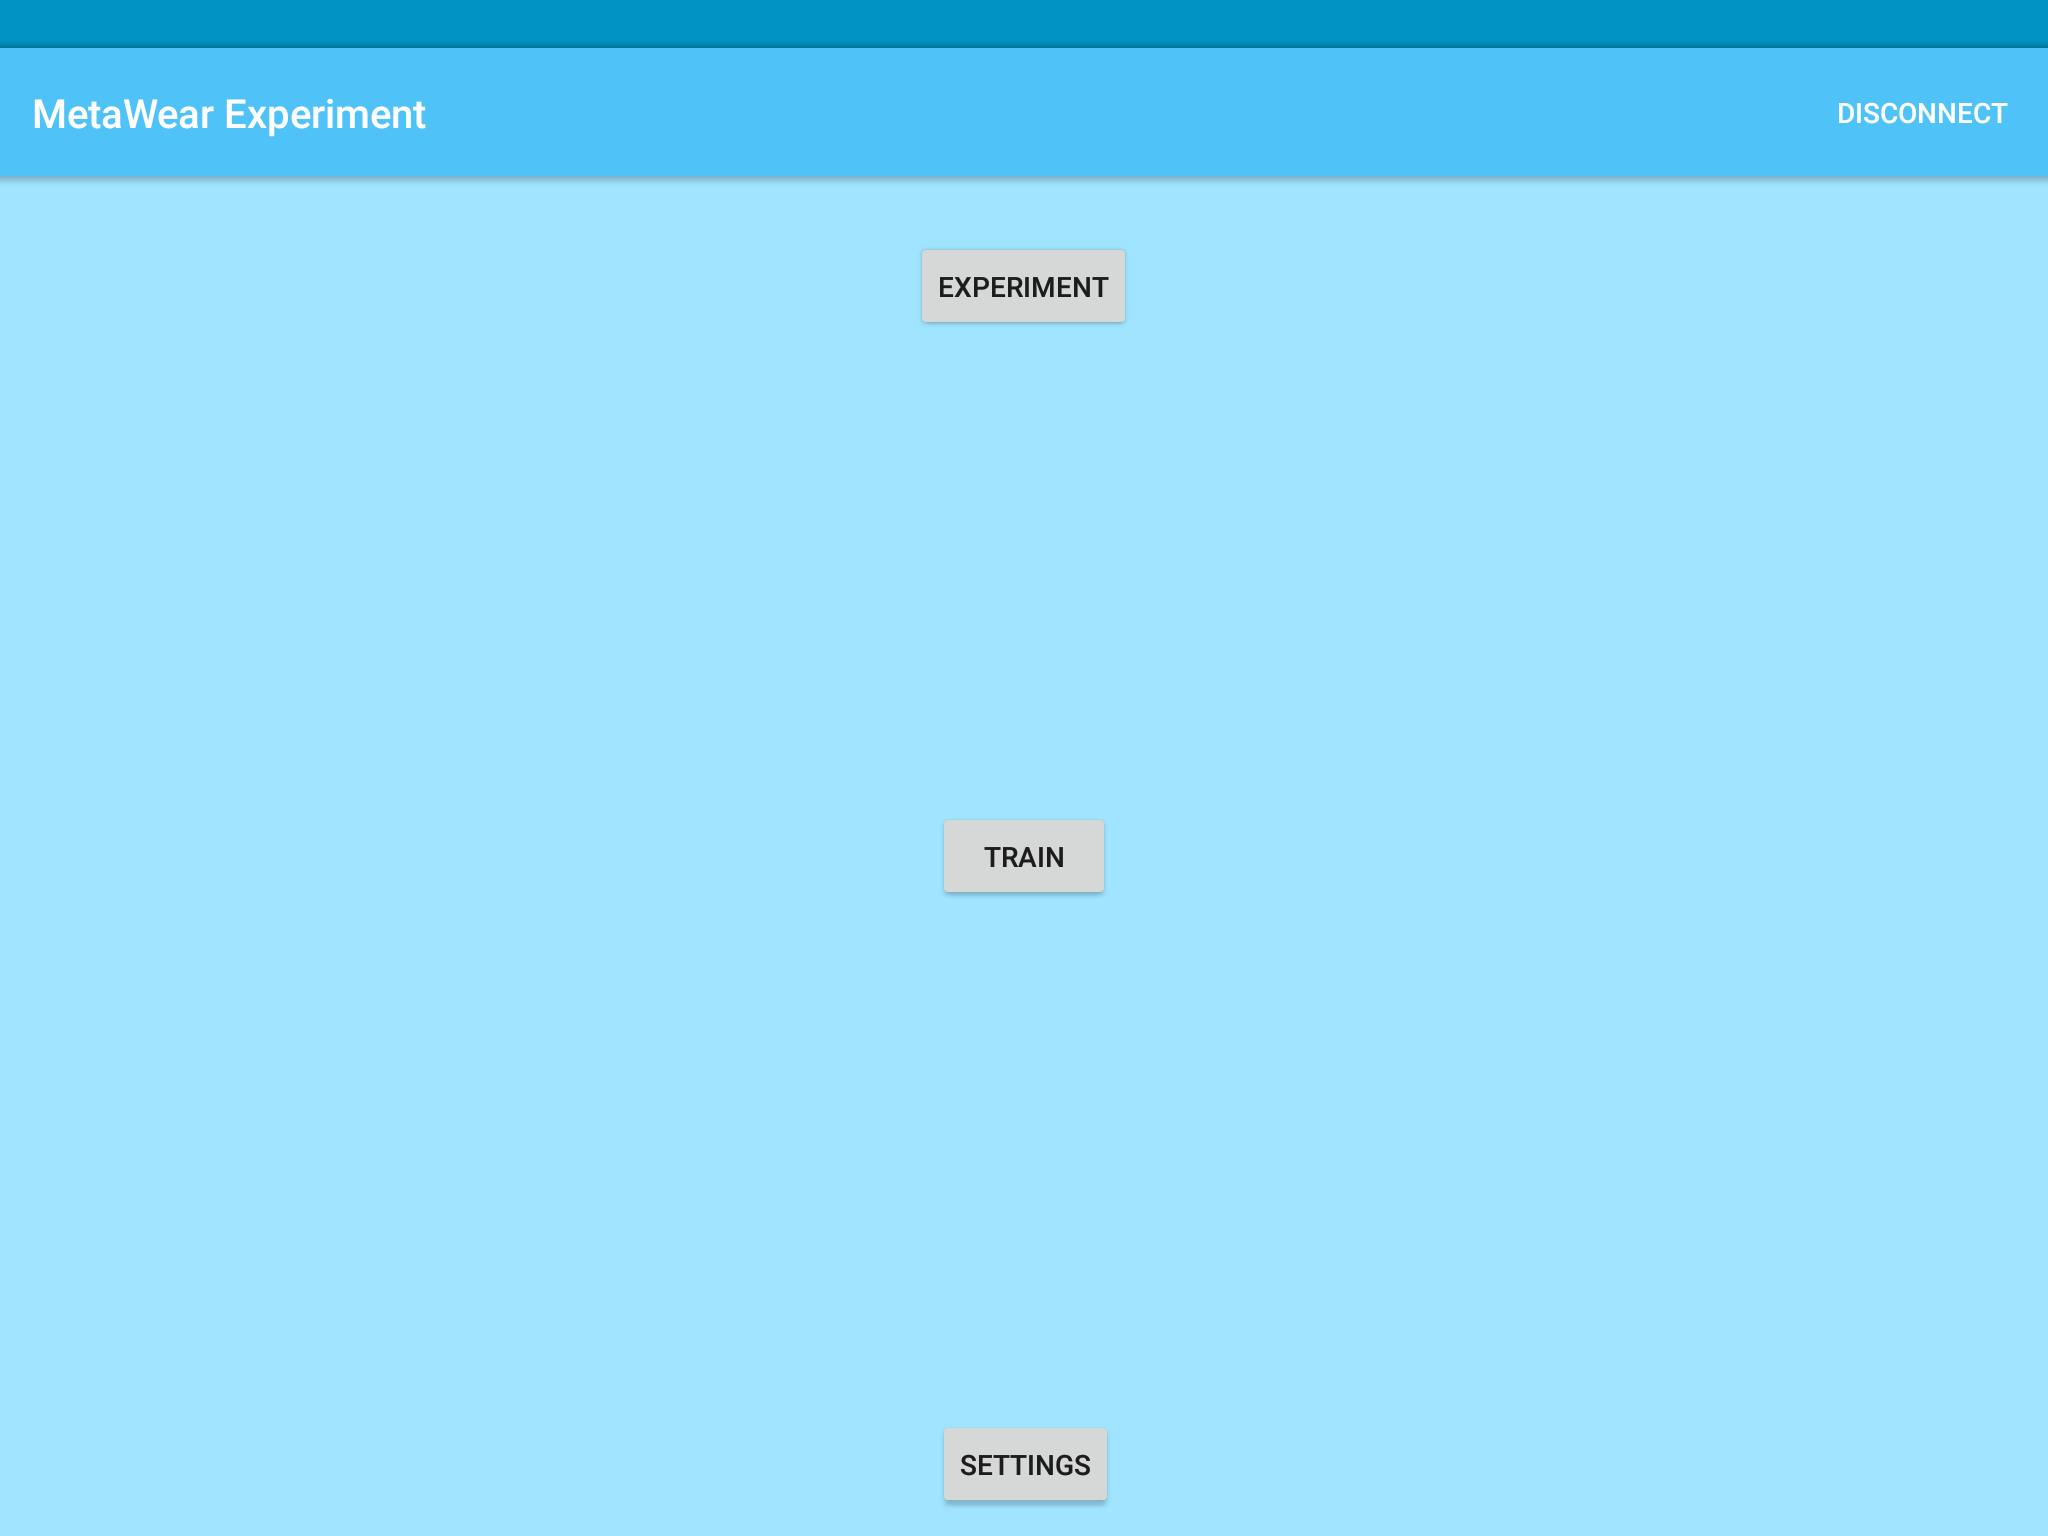
\includegraphics[width=0.95\linewidth]{figures/tablet_screen0.png}
  \captionof{figure}{Experiment app main screen}
  \label{app_main}
\end{minipage}%
\begin{minipage}{.55\textwidth}
  \centering
  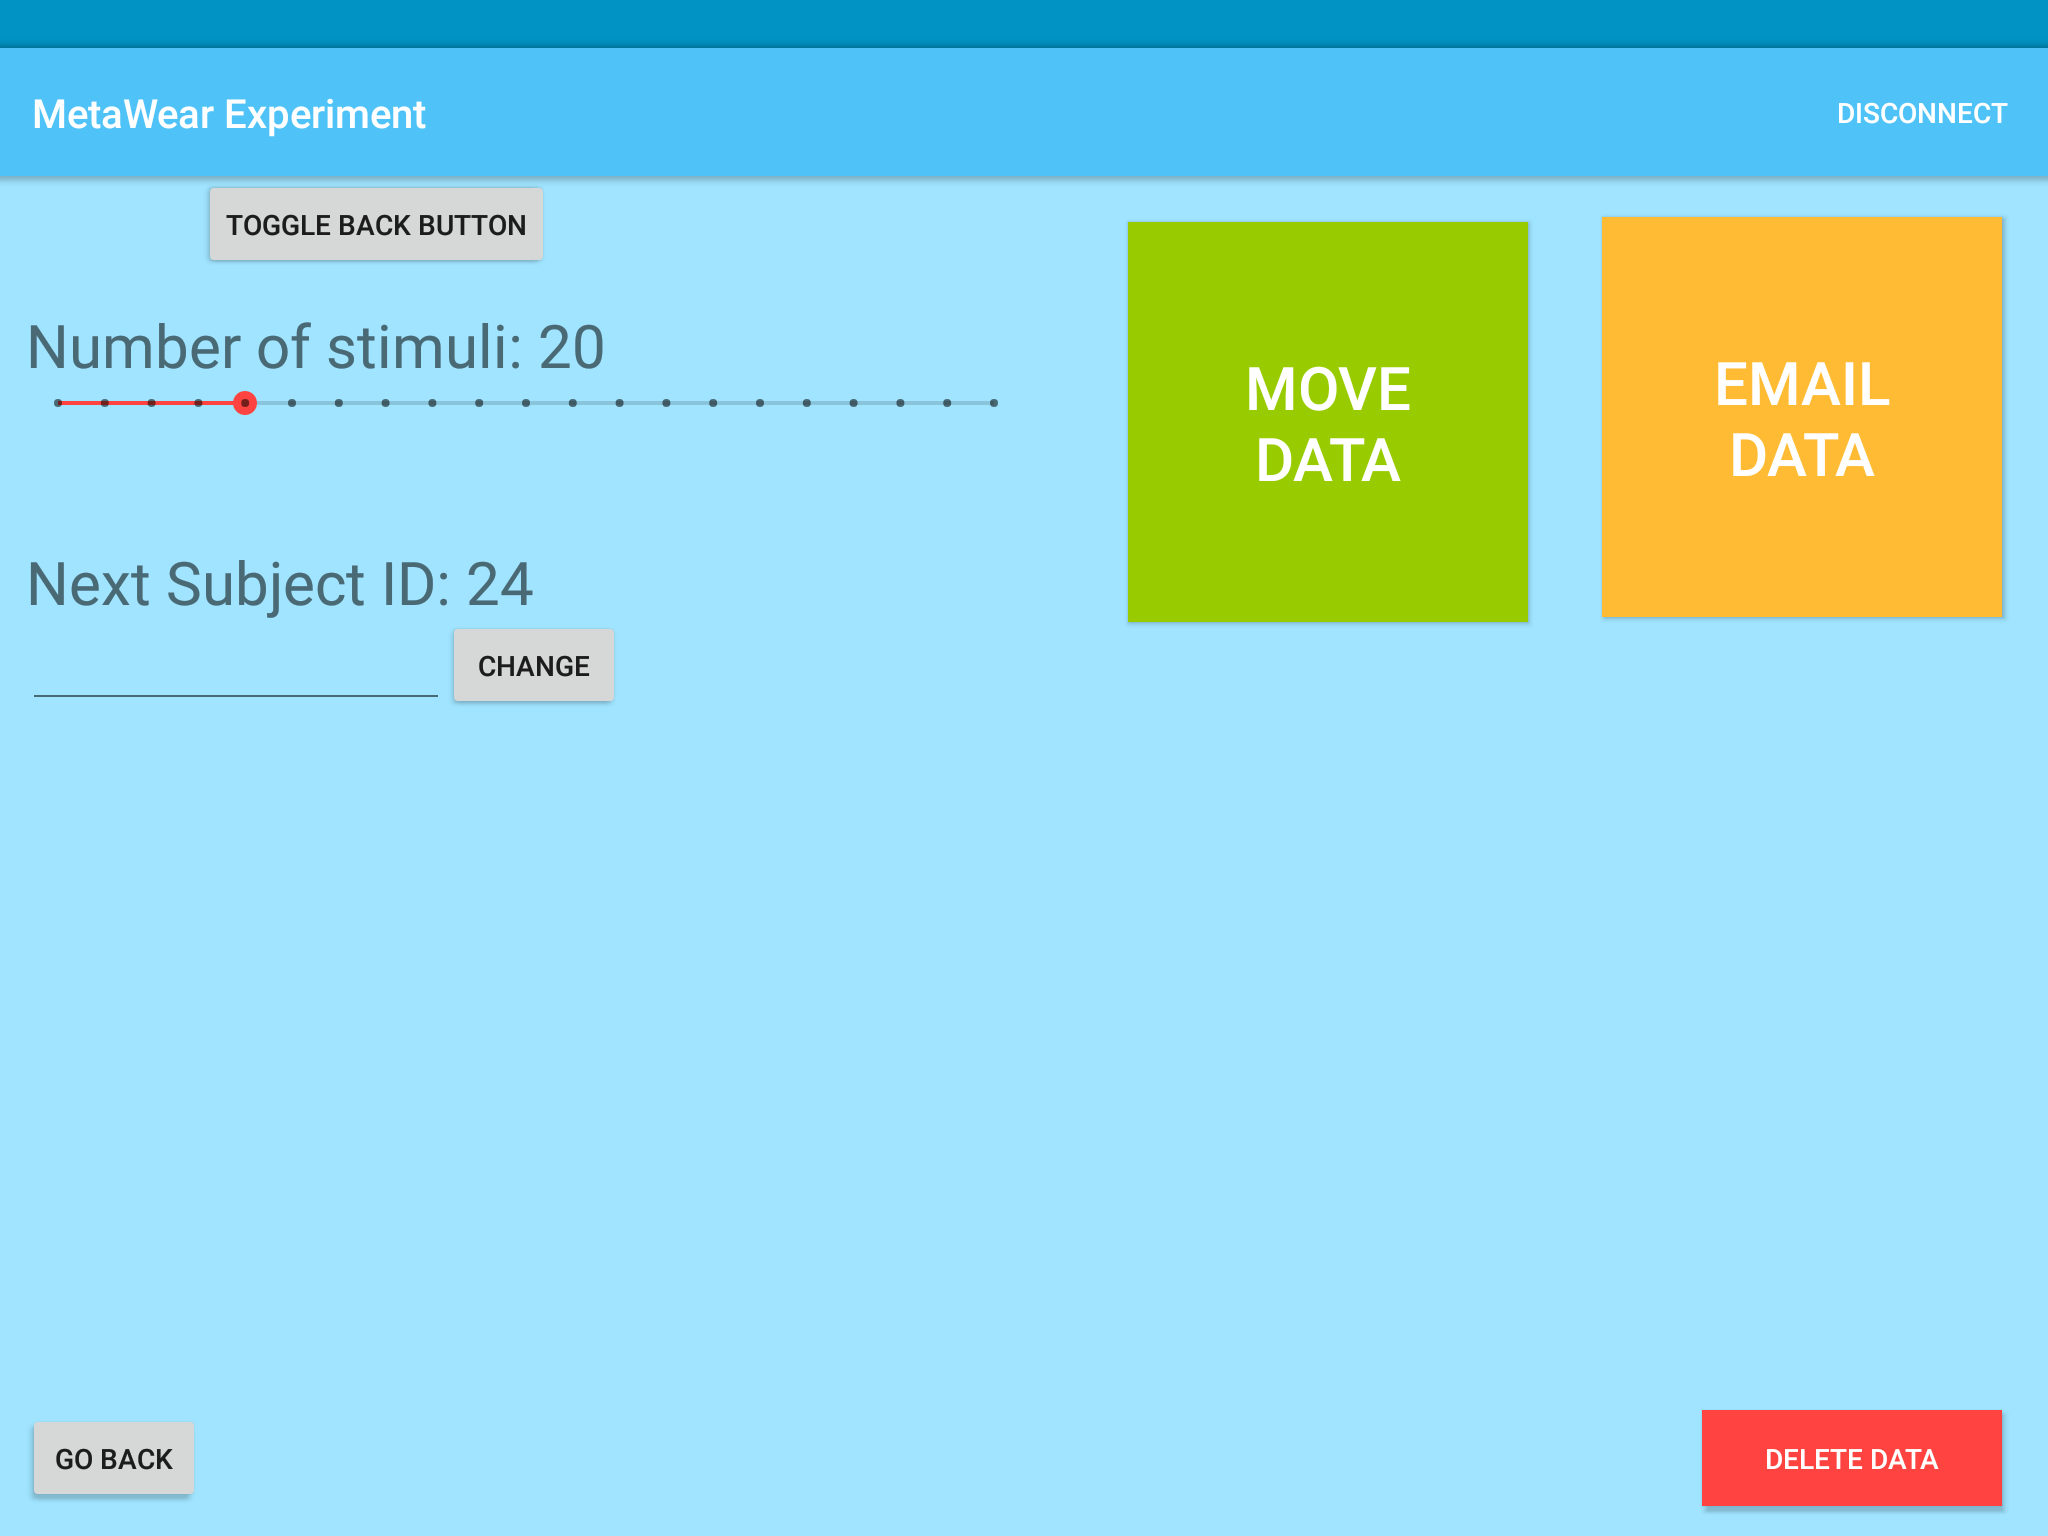
\includegraphics[width=0.95\linewidth]{figures/tablet_screen1.png}
  \captionof{figure}{Settings screen}
  \label{app_settings}
\end{minipage}
\end{figure}

The train screen is made to let the participant practice using the wristband device and get a feeling of the scale. When this screen is activated the wristband will be programmed similar as explained in Chapter \ref{implementation}, when the button is pressed it will read the orientation from its IMU and transmit it to the tablet. The light will flash and vibration motor will do a short pulse to provide feedback. The difference between the previous described implementation and the programming for the experiment is that instead of logging the data for later export, it will transmit it instantly. When the orientation data is received by the app it will map the Euler angles to a 0-10 scale and display the result. The mapping is dependant on the toggle switch, if the switch is in the \say{Hand} position as in Figure \ref{app_train_wrist} the mapping will depend on the roll angle and if the switch is in the \say{Arm} position as in Figure \ref{app_train_arm} the mapping will depend on the pitch angle. This of course correspond to the gestures described in Figure \ref{roll} and \ref{pitch}. As mentioned the roll angle will always be between -90º and 90º depending if the orientation clock or counter clock wise compared to 0º (horizontal). To map the values to a 0-10 scale the absolute value is divided by 9, e.g 90º/-90º will become 10, 45º/-45º will become 5, 25º/-25º will become 2.7778 etc. Mathematically this can be expressed with this function where \emph{sv} is the scaled value from 0-10 and \emph{ra} is the Euler angle for the roll axis:
\begin{center}
$sv\left ( ra \right ) = \frac{abs\left (ra\right )}{9}$
\end{center}

A consequence of this mapping is that if the participant turn the wristband pass the vertical position the scaled value will begin to decrease. This means that the participant won't achieve a 10 rating simply by turning the wrist way beyond the vertical position. A different solution could be made to detect when the wristband pass the vertical position and set the scaled value at 10. It can be debated as to which solution is the greater, but by letting the scaled value decrease will force the participant to get a better sense of the scale and won't allow \say{lazy} responses.

Mapping the pitch angle is a little more complicated, since the roll value will be between -180º and 180º. The soltuion is to create a function that maps the value differently depending if the absolute pitch angle is greater than 90, basically first mapping the -180º to 180º range down to a -90º to 90º degree range, and then mapping it to the scaled value. This function will express this where \emph{sv} is the scaled value from 0-10 and \emph{pa} is the Euler angle for the pitch axis:
\begin{center}
$sv\left ( pa \right ) = \left\{\begin{matrix}
\frac{90-\left ( abs\left ( pa \right )-90 \right )}{9} & if\ pa> 90 \\ 
\frac{abs\left ( pa \right )}{9} & otherwise
\end{matrix}\right.$
\end{center}

This mapping has the same property as explained before, where if the pitch angle goes pass the vertical position the scaled value will decrease.




\begin{figure}[h!]
\centering
\begin{minipage}{.55\textwidth}
  \centering
  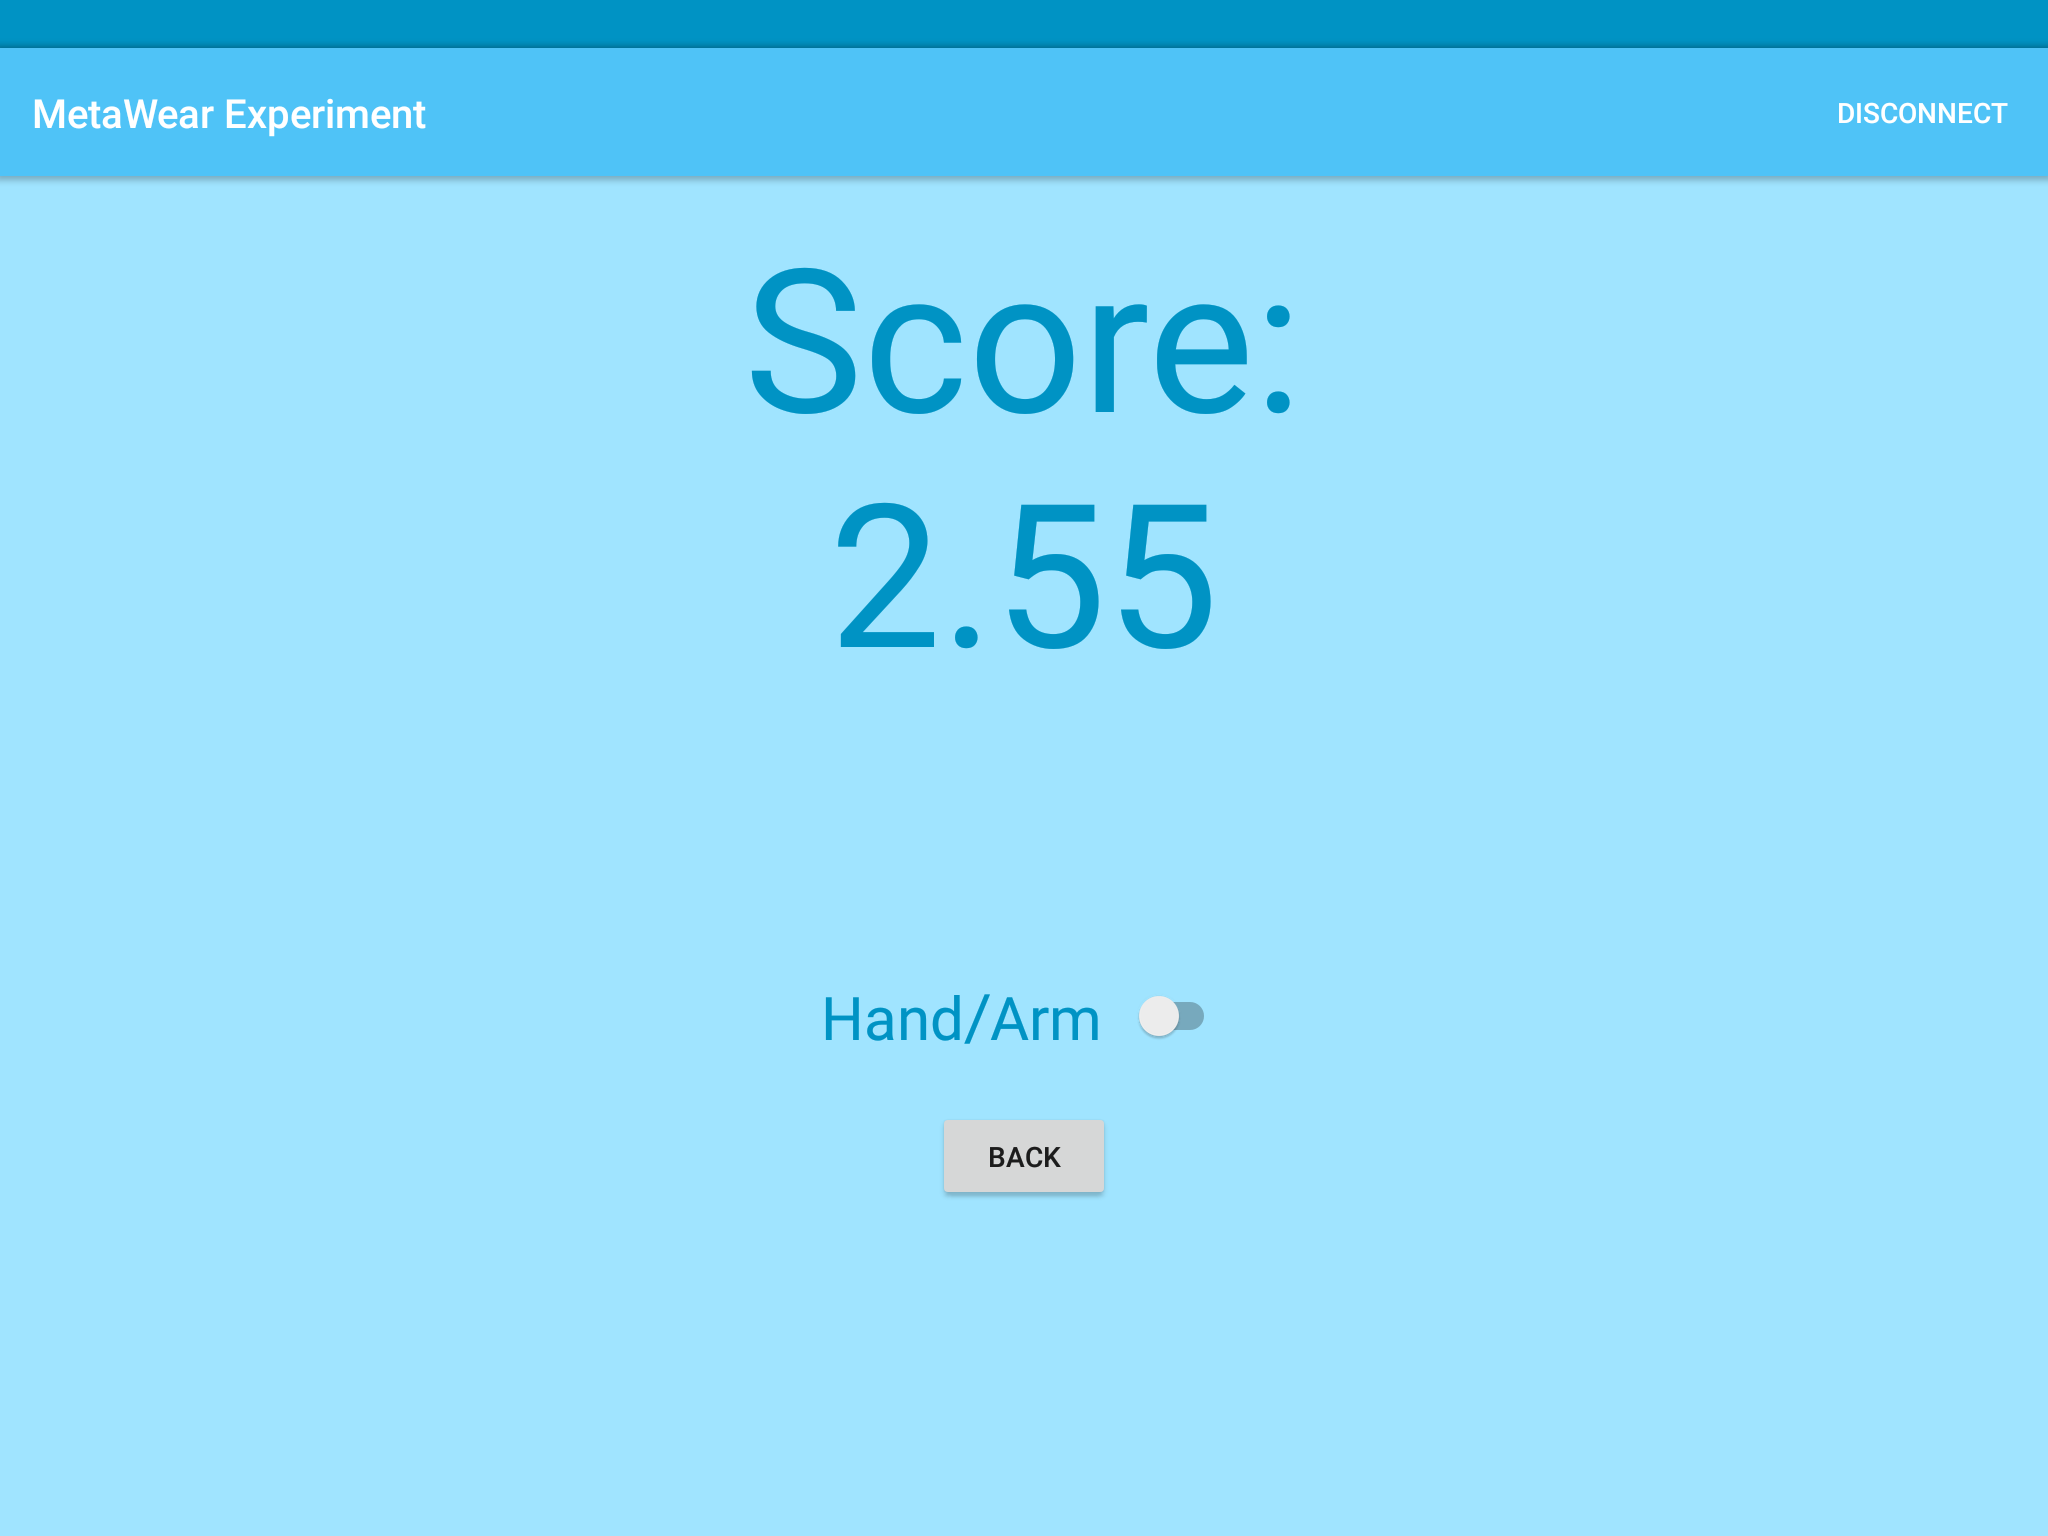
\includegraphics[width=0.95\linewidth]{figures/tablet_screen3.png}
  \captionof{figure}{Train screen hand (wrist) mode}
  \label{app_train_wrist}
\end{minipage}%
\begin{minipage}{.55\textwidth}
  \centering
  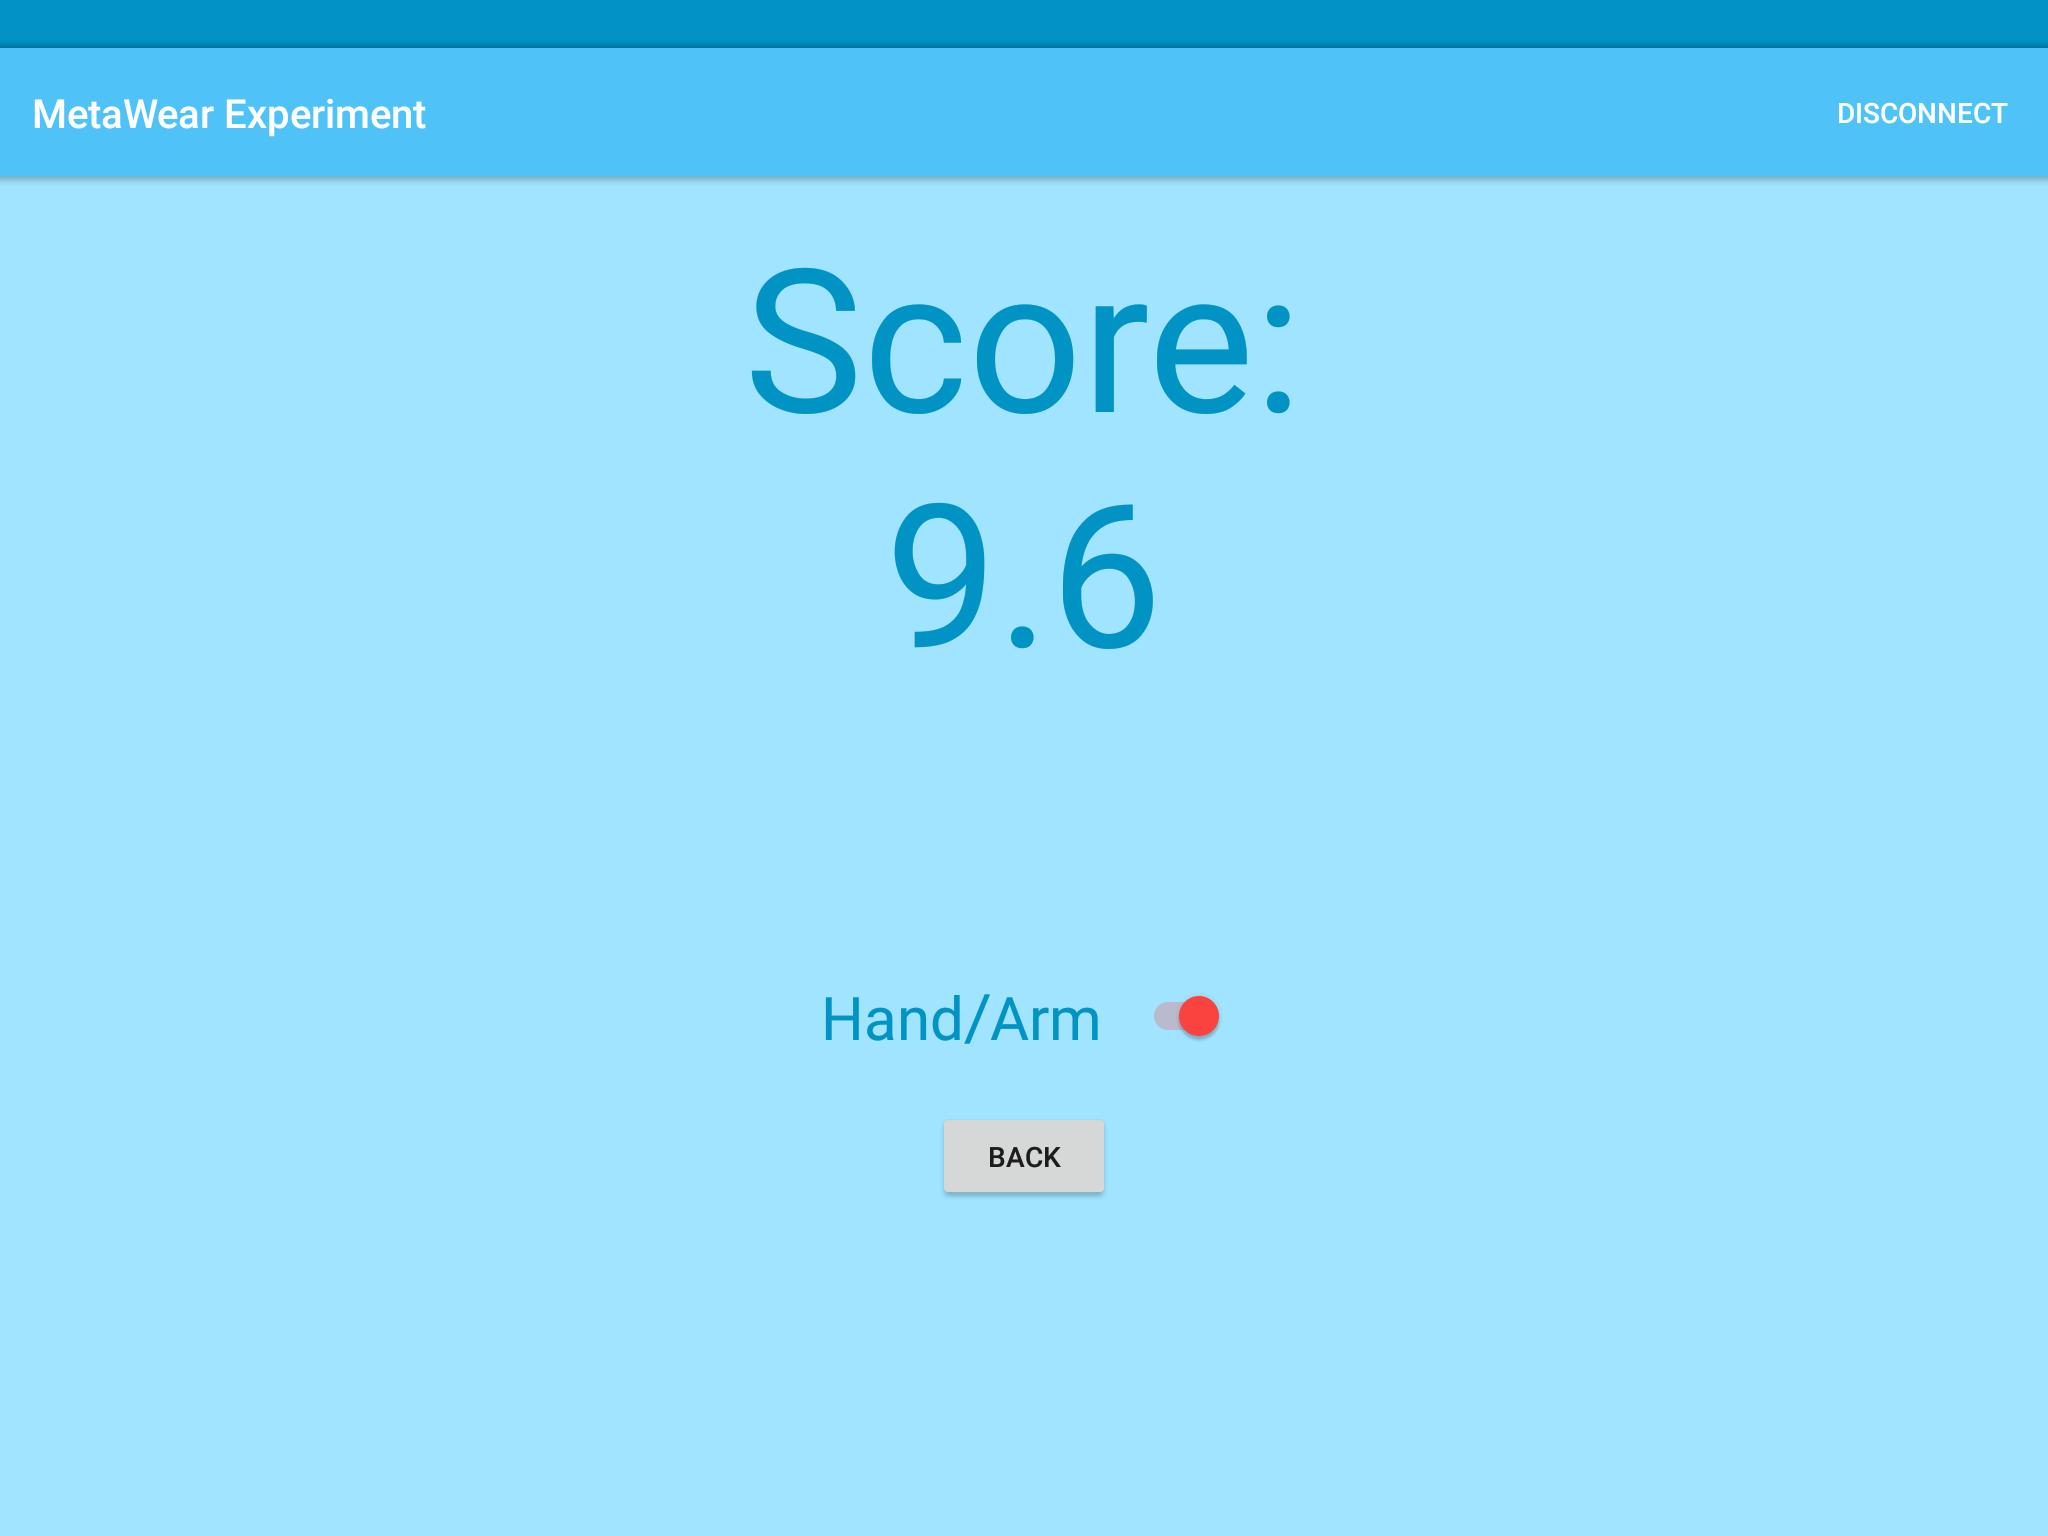
\includegraphics[width=0.95\linewidth]{figures/tablet_screen4.png}
  \captionof{figure}{Train screen arm mode}
  \label{app_train_arm}
\end{minipage}
\end{figure}

The last screen is the experiment itself, this is the most complicated screen and consist of many \say{sub screens}. Before the experiment begin a screen for inputting the gender and age of the participant is presented as seen in Figure \ref{app_ex_start}. In the top right the assigned ID for the participant is showed, this is just for confirmation and to be used in the survey after the experiment (so the survey and experiment data can be synchronized if needed). Once the \say{Start} button is pressed the experiment will begin. As mentioned the experiment consist of six exercises and the order of these is dependent on Table \ref{latin}. Before each exercise an explanation screen will show, this screen will have some text to explain the task of the exercise and a short GIF that illustrates it. The text will stay on top during the whole exercise. This screen purpose is to make sure the participant is sure of what task they are required to do, the participant will have gotten instructions beforehand, so this screen is just reassure them. Three of the six explanation screens can be seen in Figure \ref{app_slider_explain}, \ref{app_arm_explain} and \ref{app_wrist_explain}.

\begin{figure}[h!]
\centering
\begin{minipage}{.55\textwidth}
  \centering
  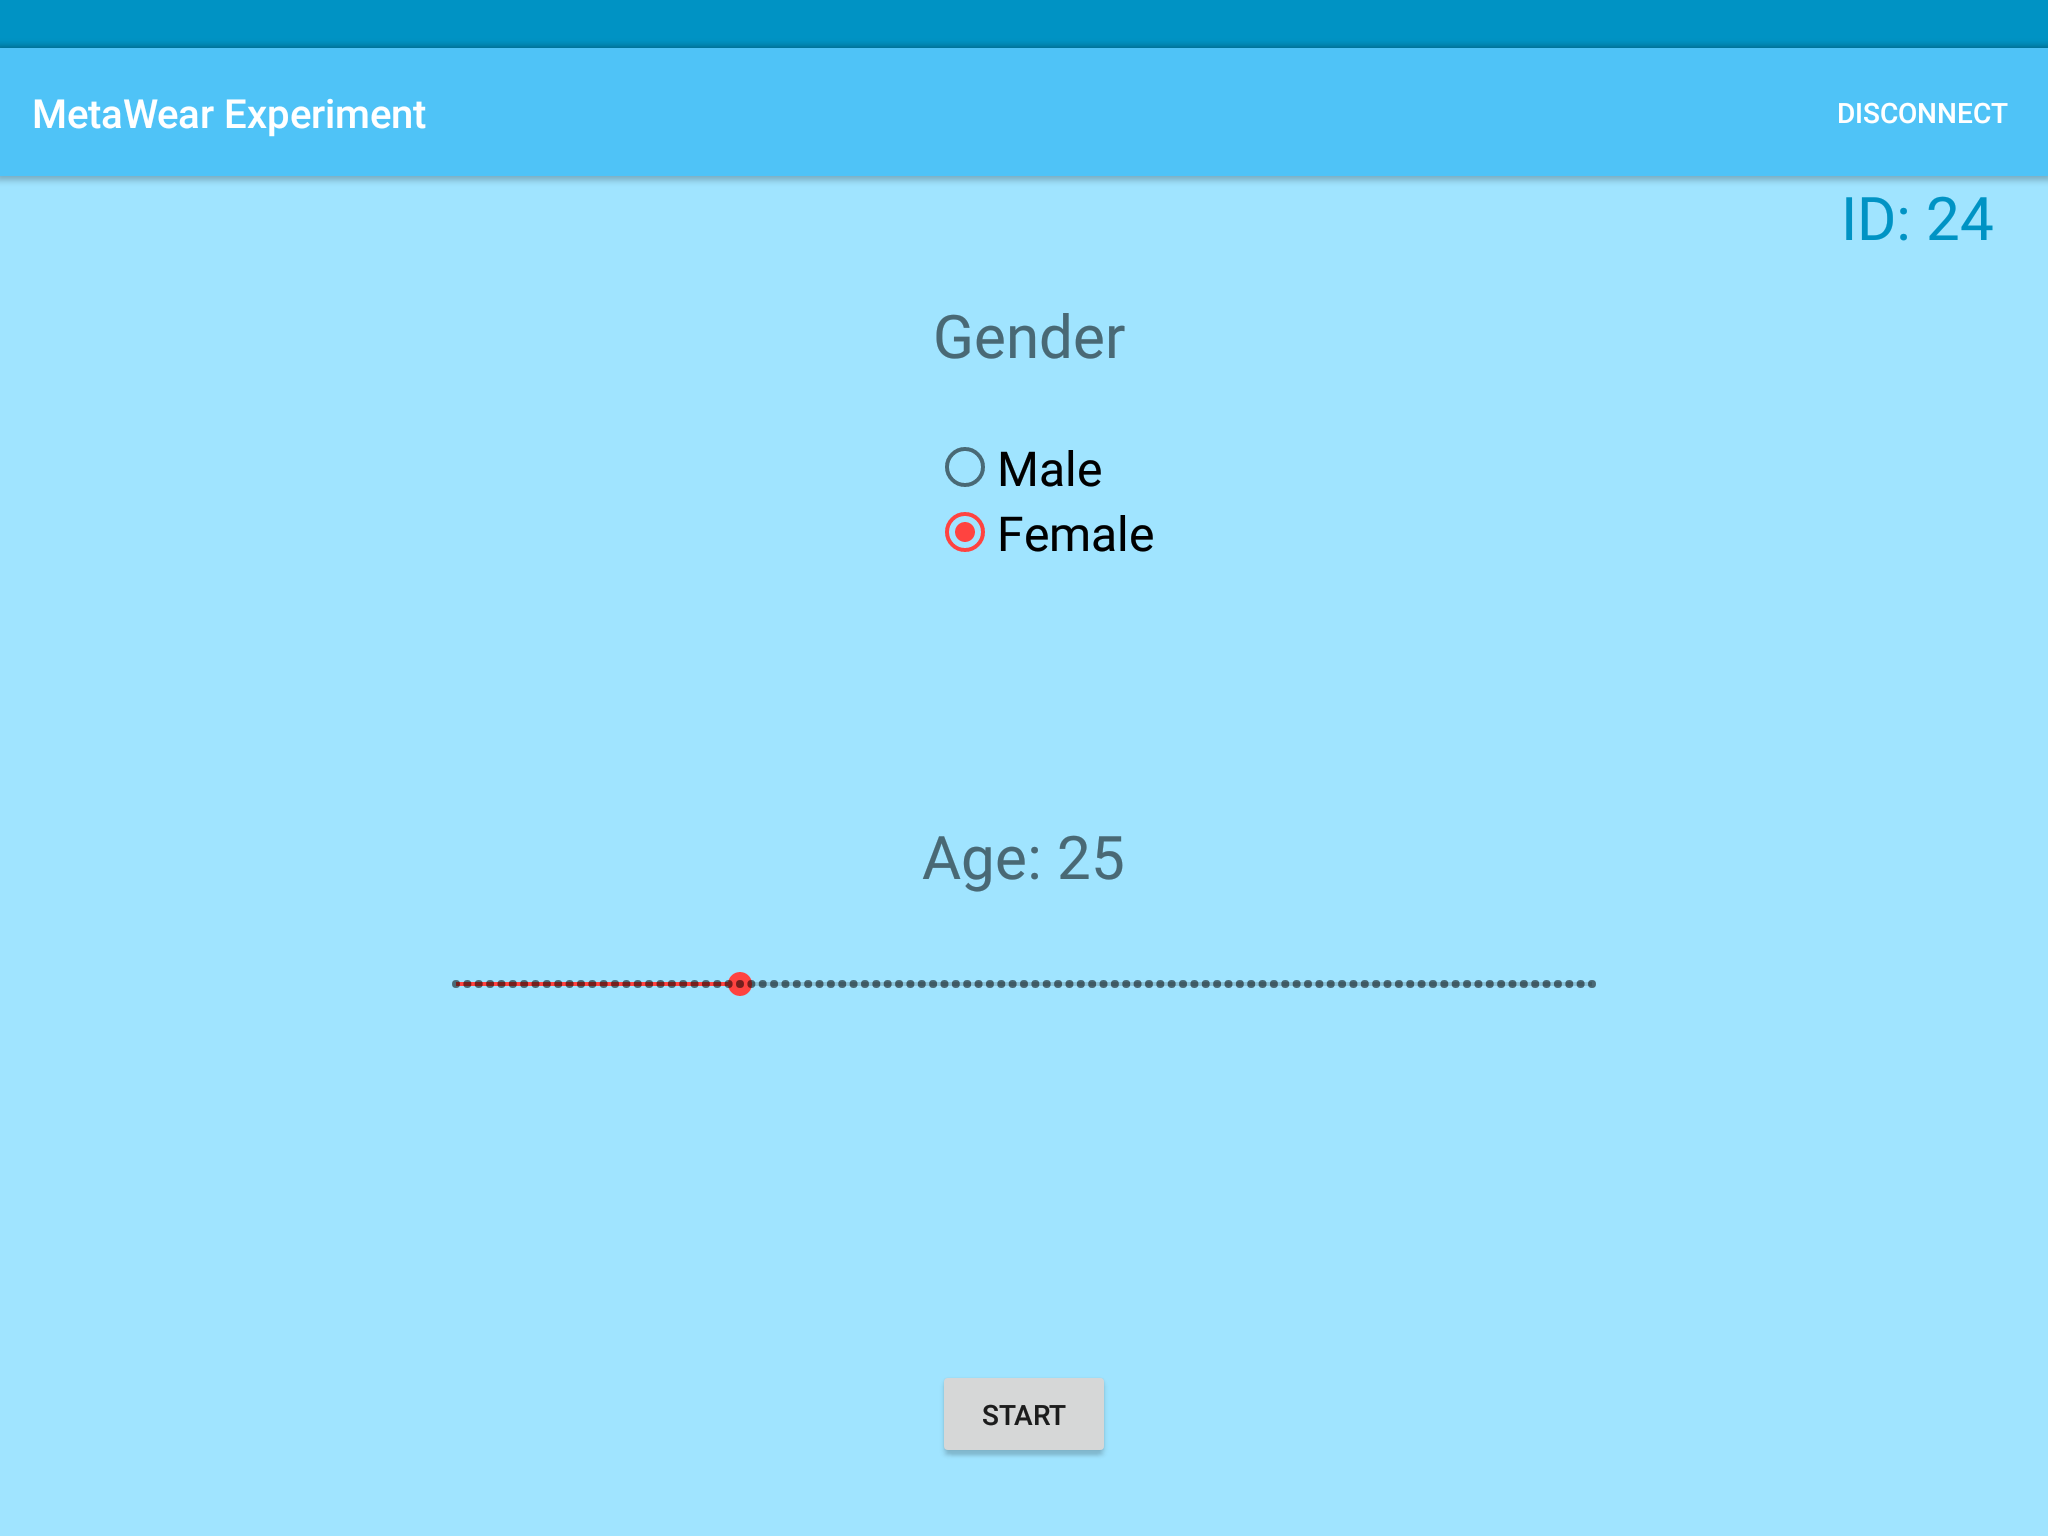
\includegraphics[width=0.95\linewidth]{figures/tablet_screen5.png}
  \captionof{figure}{Experiment start screen}
  \label{app_ex_start}
\end{minipage}%
\begin{minipage}{.55\textwidth}
  \centering
  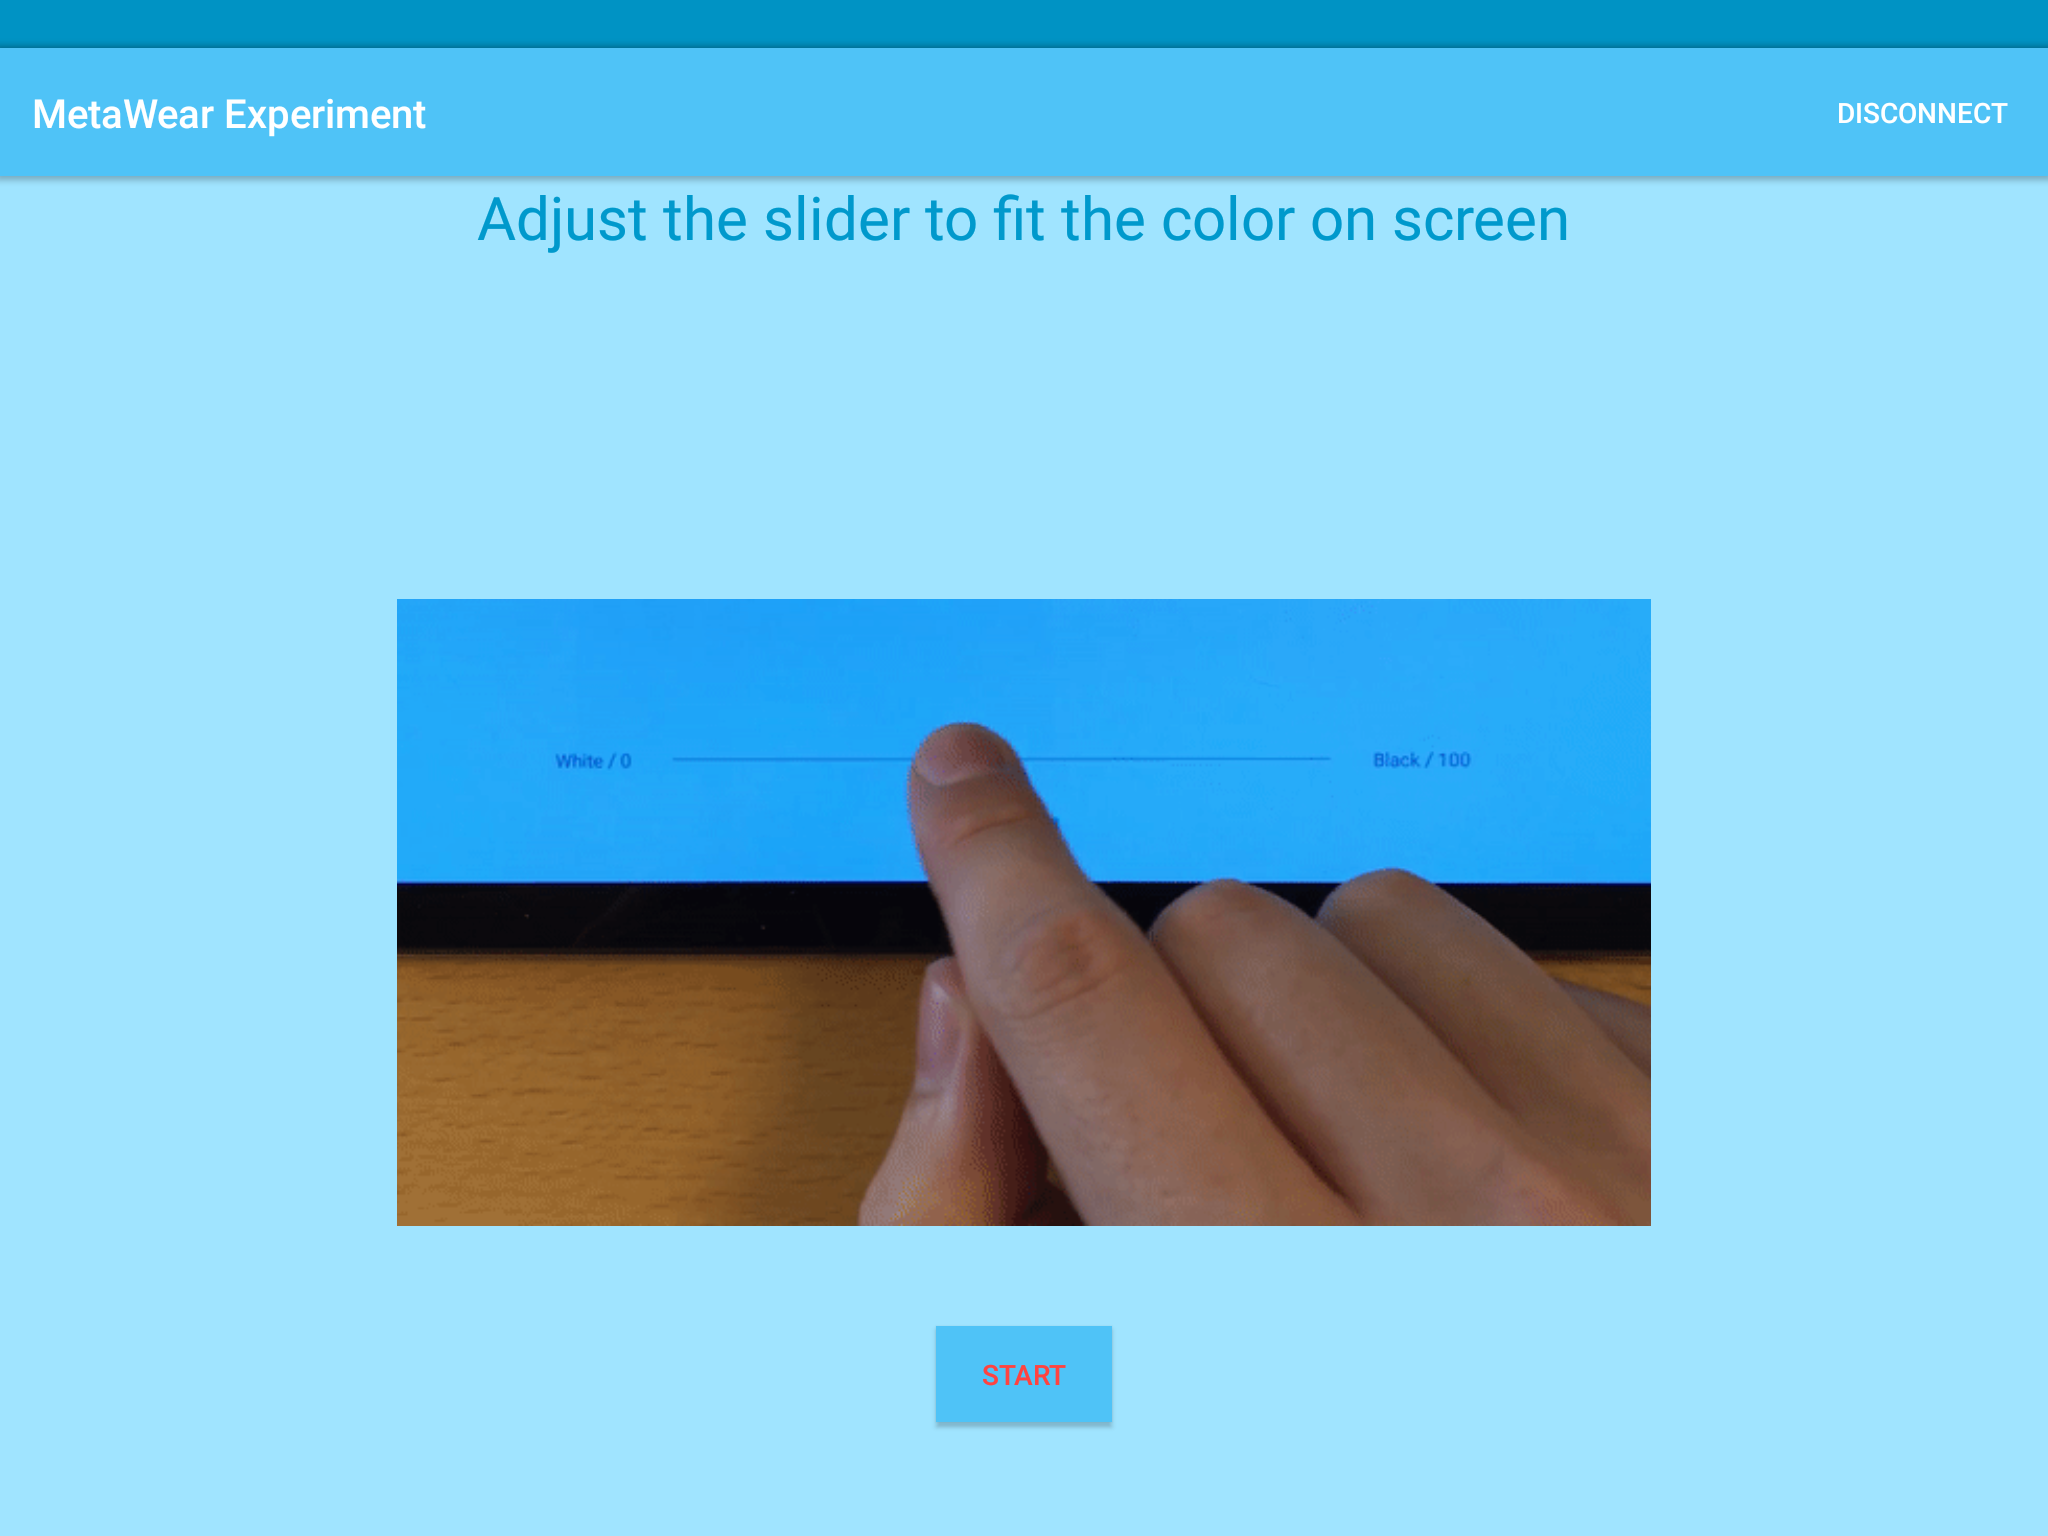
\includegraphics[width=0.95\linewidth]{figures/tablet_screen6.png}
  \captionof{figure}{slider\_grey explanation screen}
  \label{app_slider_explain}
\end{minipage}
\end{figure}

\begin{figure}[h!]
\centering
\begin{minipage}{.55\textwidth}
  \centering
  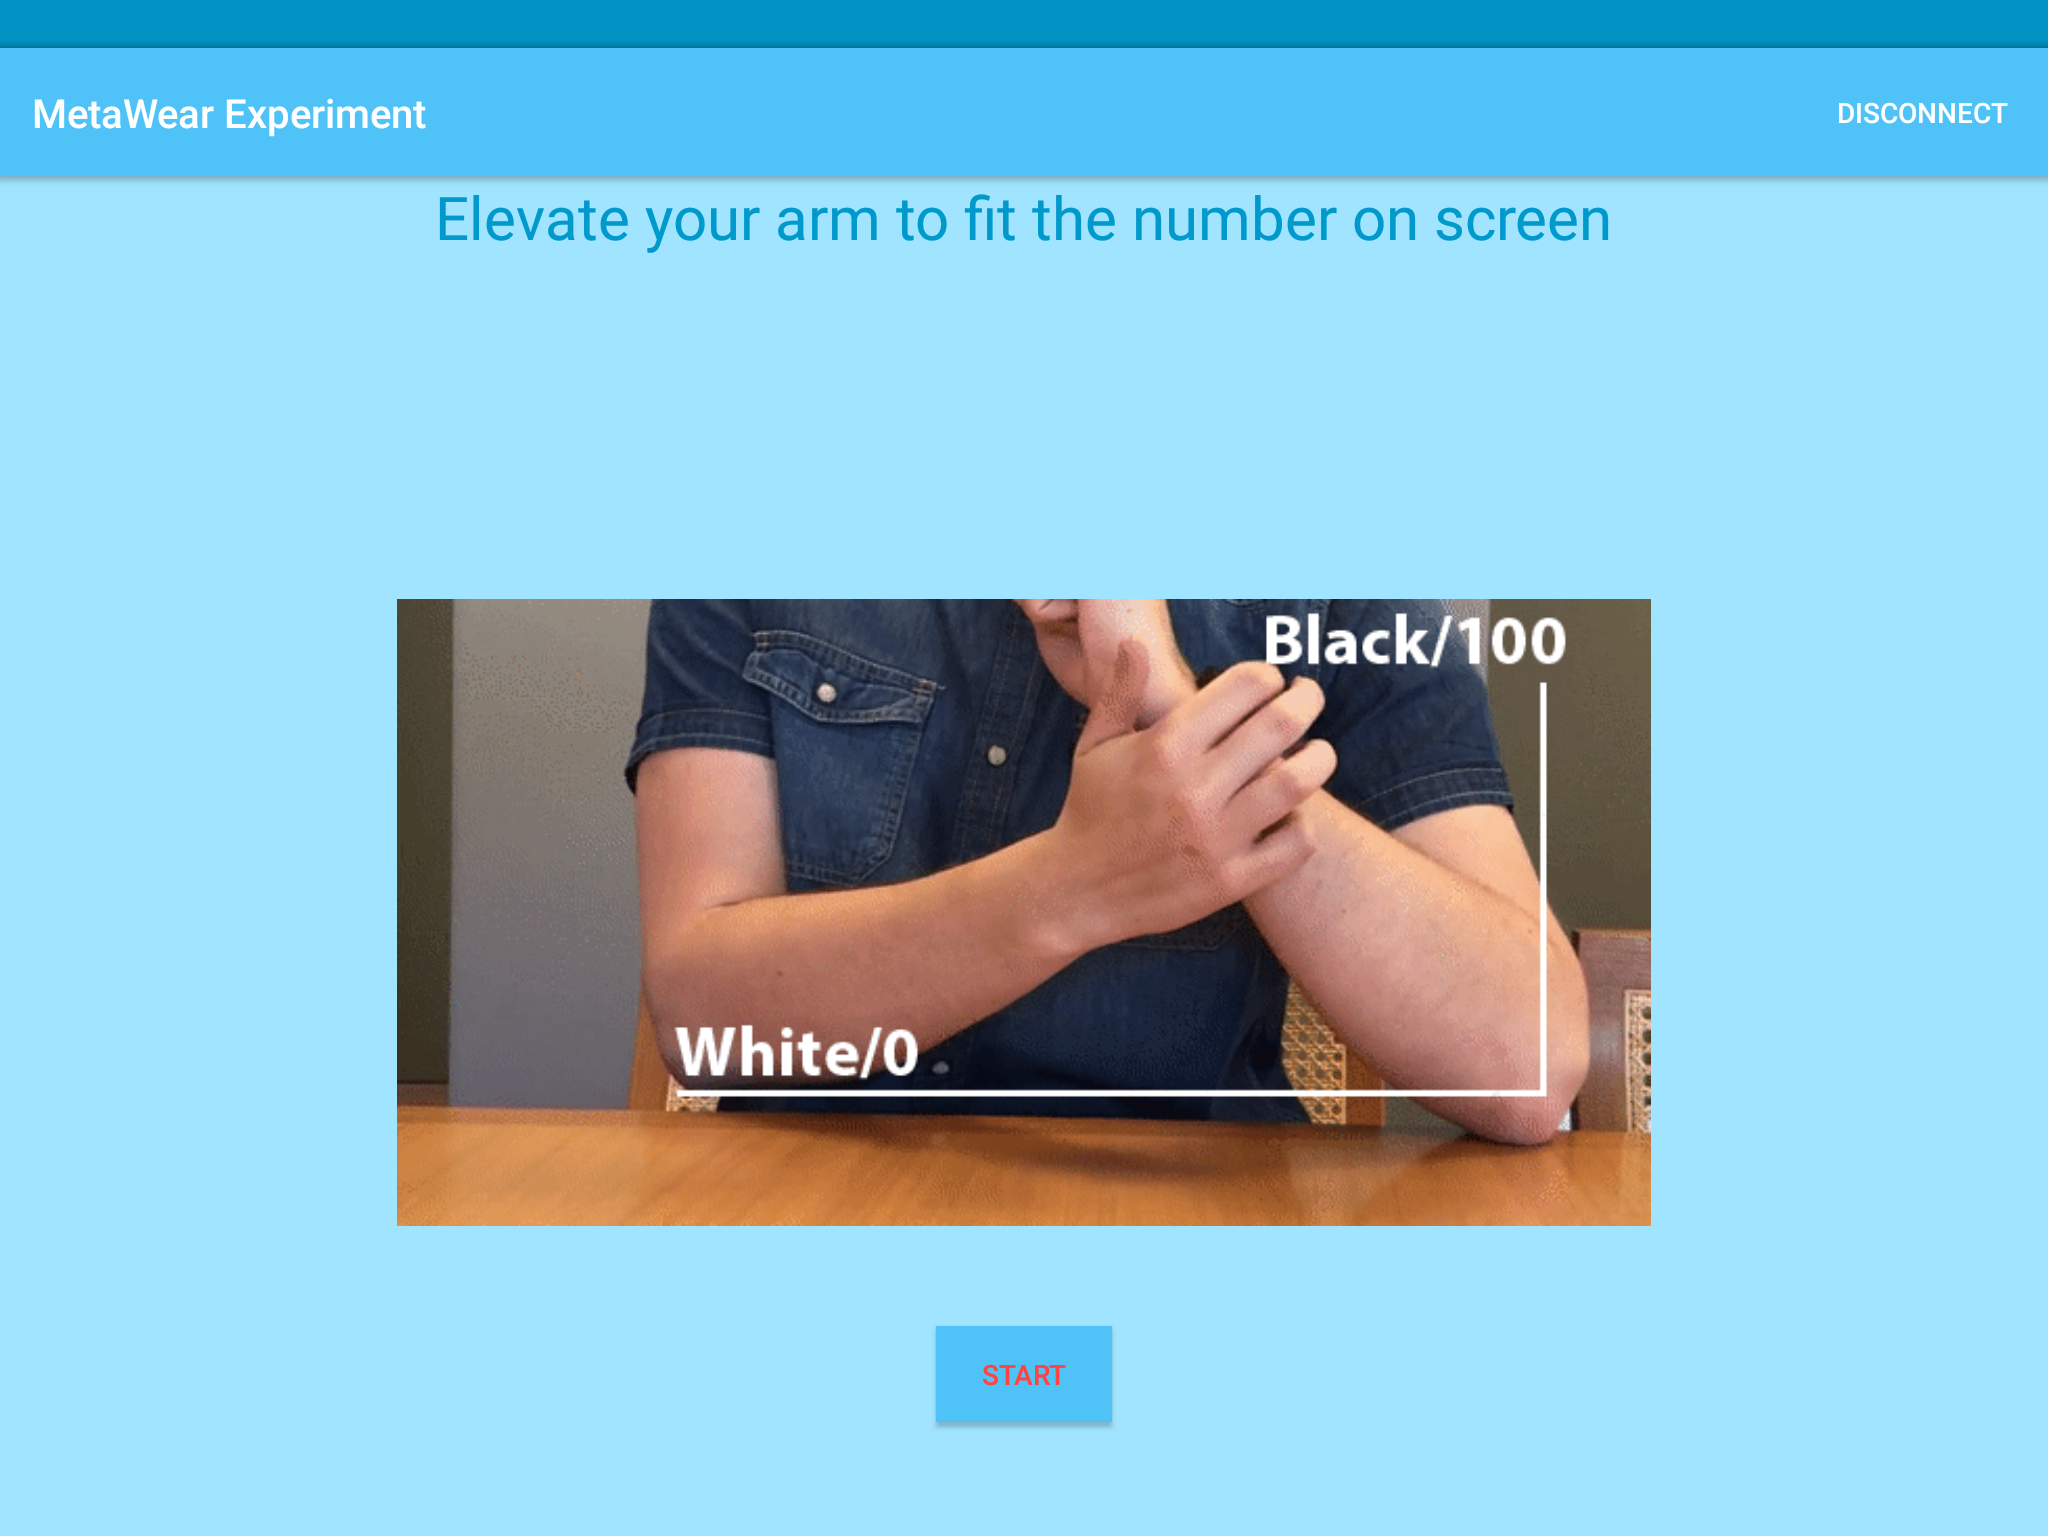
\includegraphics[width=0.95\linewidth]{figures/tablet_screen12.png}
  \captionof{figure}{arm\_num explanation screen}
  \label{app_arm_explain}
\end{minipage}%
\begin{minipage}{.55\textwidth}
  \centering
  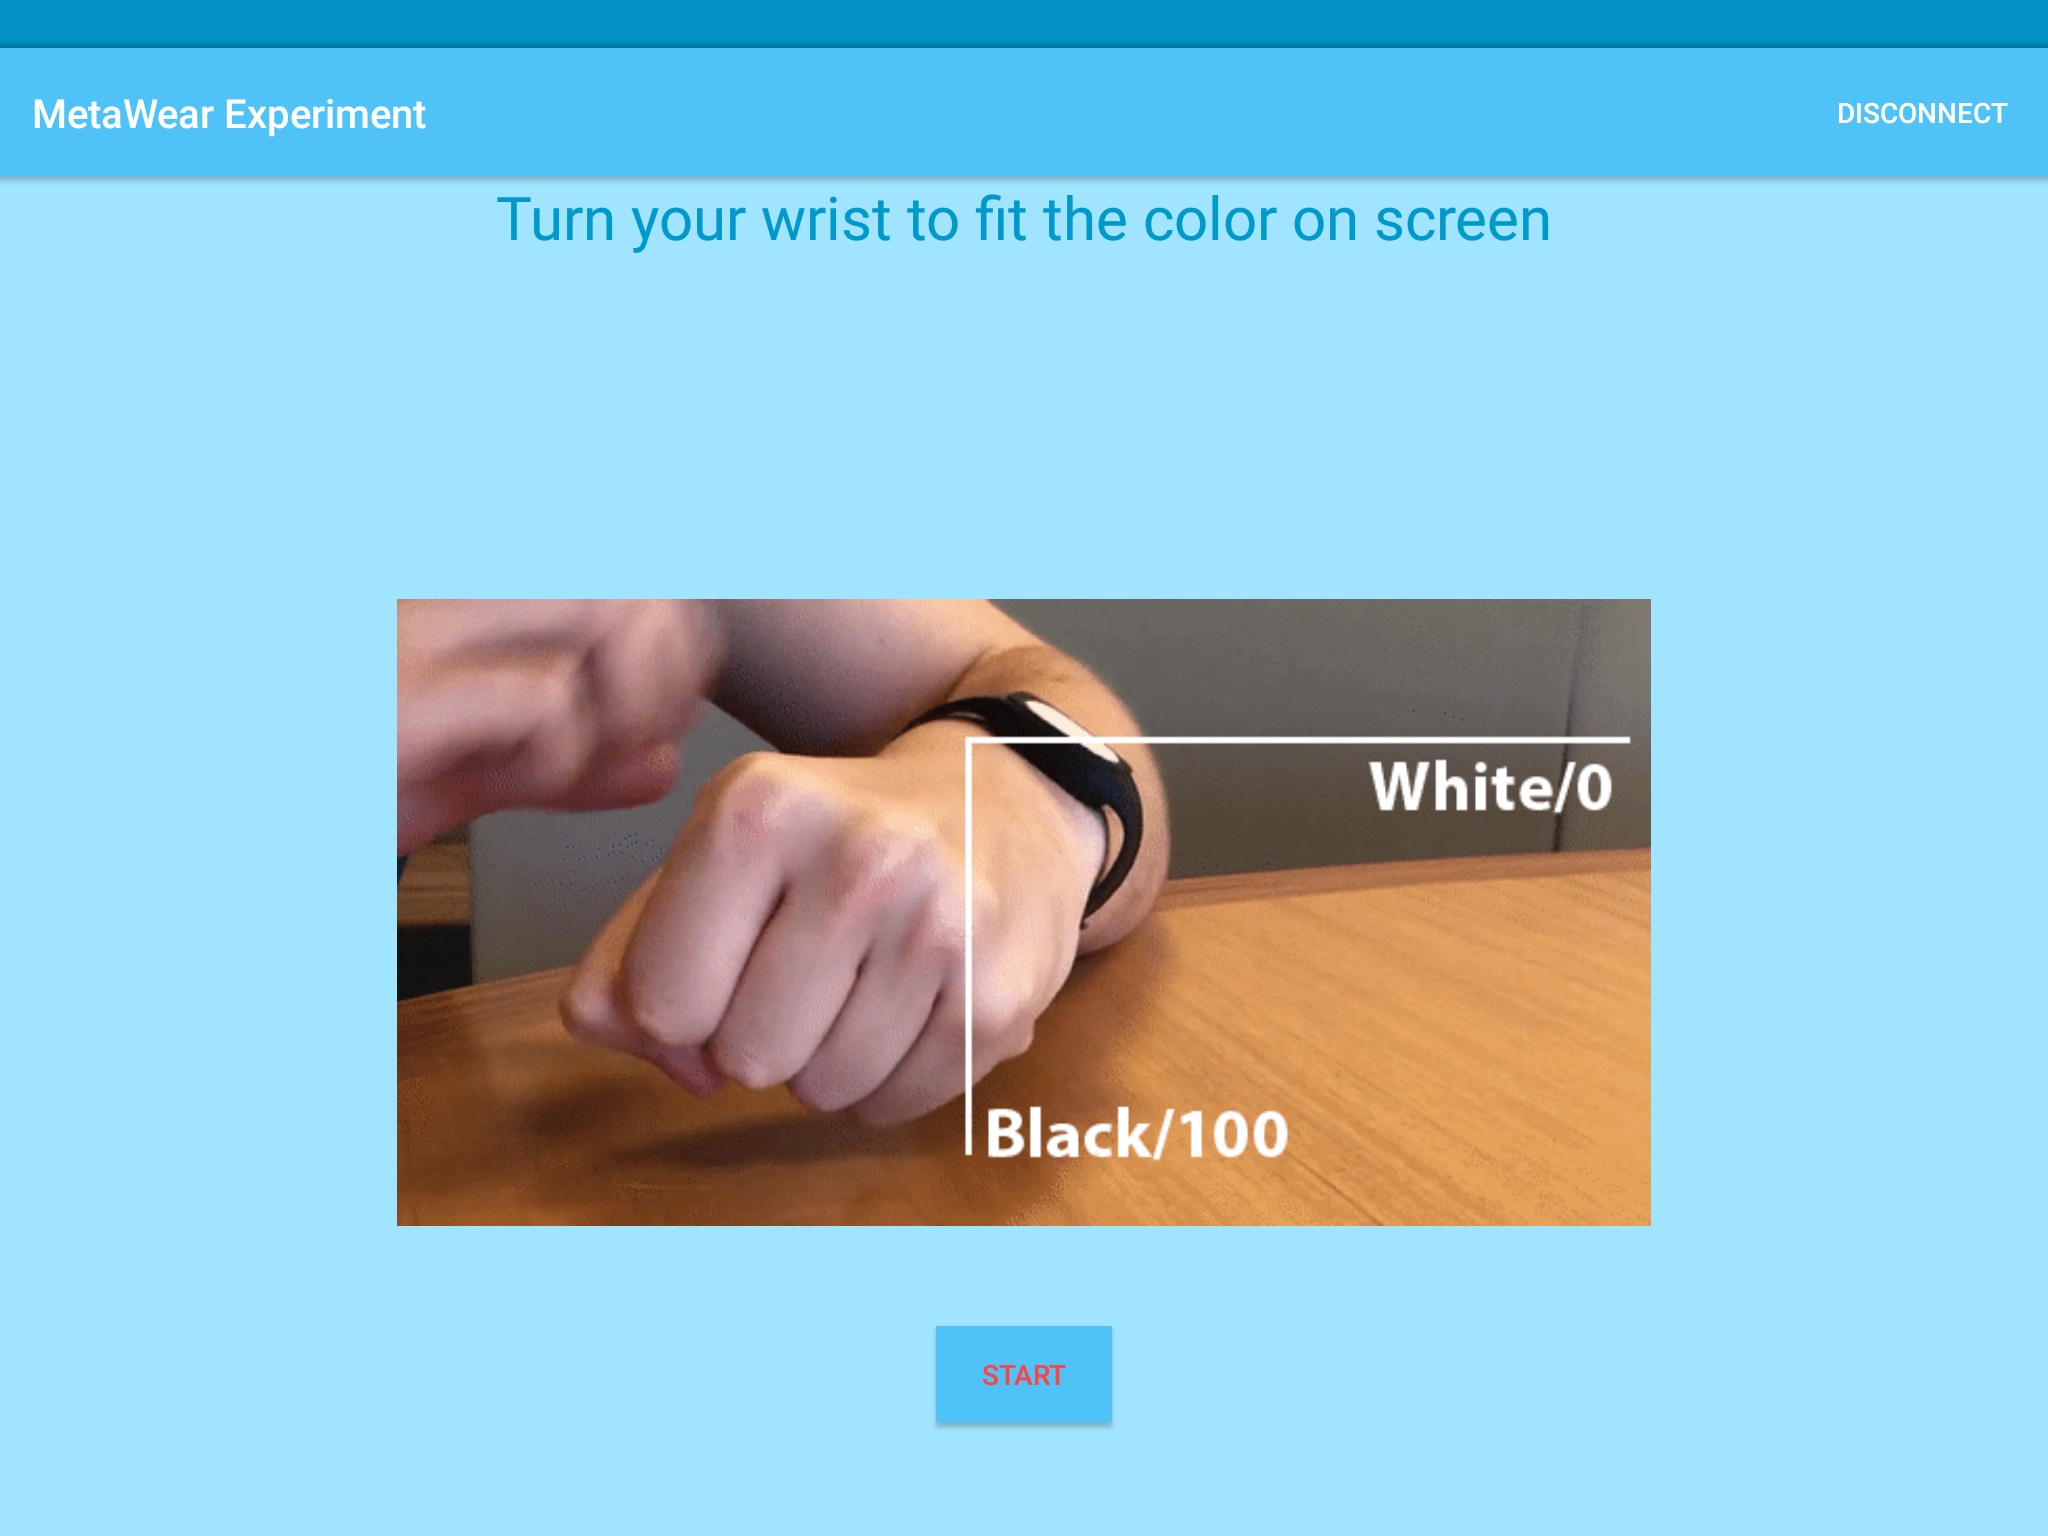
\includegraphics[width=0.95\linewidth]{figures/tablet_screen13.png}
  \captionof{figure}{wrist\_grey explanation screen}
  \label{app_wrist_explain}
\end{minipage}
\end{figure}

After the explanation screen each exercise follow the same pattern: show stimuli, wait for input, refresh input (optional), register input, next input. This pattern is repeated until the set number of stimuli has been shown and then the next exercise is started, after all six exercises are completed a \say{finish} screen is shown. The slider\_grey exercise will be used to explain this pattern in more detail. After the exercise explanation the first stimuli is shown as seen in Figure \ref{app_show_stim}, then the participant registers a input using the slider as seen in Figure \ref{app_input_slider}, a small vertical bar indicate the input. The input can be changed simply by adjusting the slider (for arm and wrist exercises the participant can just press the button on the wristband again), to register the input the participant has to press the \say{Submit} button as seen in Figure \ref{app_input_slider}. Once the input has been registered the stimuli will disappear and the participant has to press the \say{Next} button as seen in Figure \ref{app_next_stim}, this button will alternate to appear on the left and right side of the screen (this will be explained later), once the button has been pressed the next stimuli will appear (as seen in Figure \ref{app_repeat})and the process will repeat until the participant has been through the set amount of stimuli and moves on to the next exercise. In Figure \ref{app_wrist_int} we see a screen from the wrist\_num exercise where the participant has pressed the button on the wristband, beside the feedback from the wristband (light and vibration) the screen also show that the button has been pressed, but no feedback is given on what value was registered nor how well they performed. This was done on purpose to reflect the real life use case where the user wouldn't know the registered value before importing it to the companion app. In Figure \ref{app_finish} we see the \say{Finish} screen after the participant has completed the experiment. All app screens shown here plus a couple extra can be seen in larger scale in Appendix \ref{ex_app_screens}.

\begin{figure}[h!]
\centering
\begin{minipage}{.55\textwidth}
  \centering
  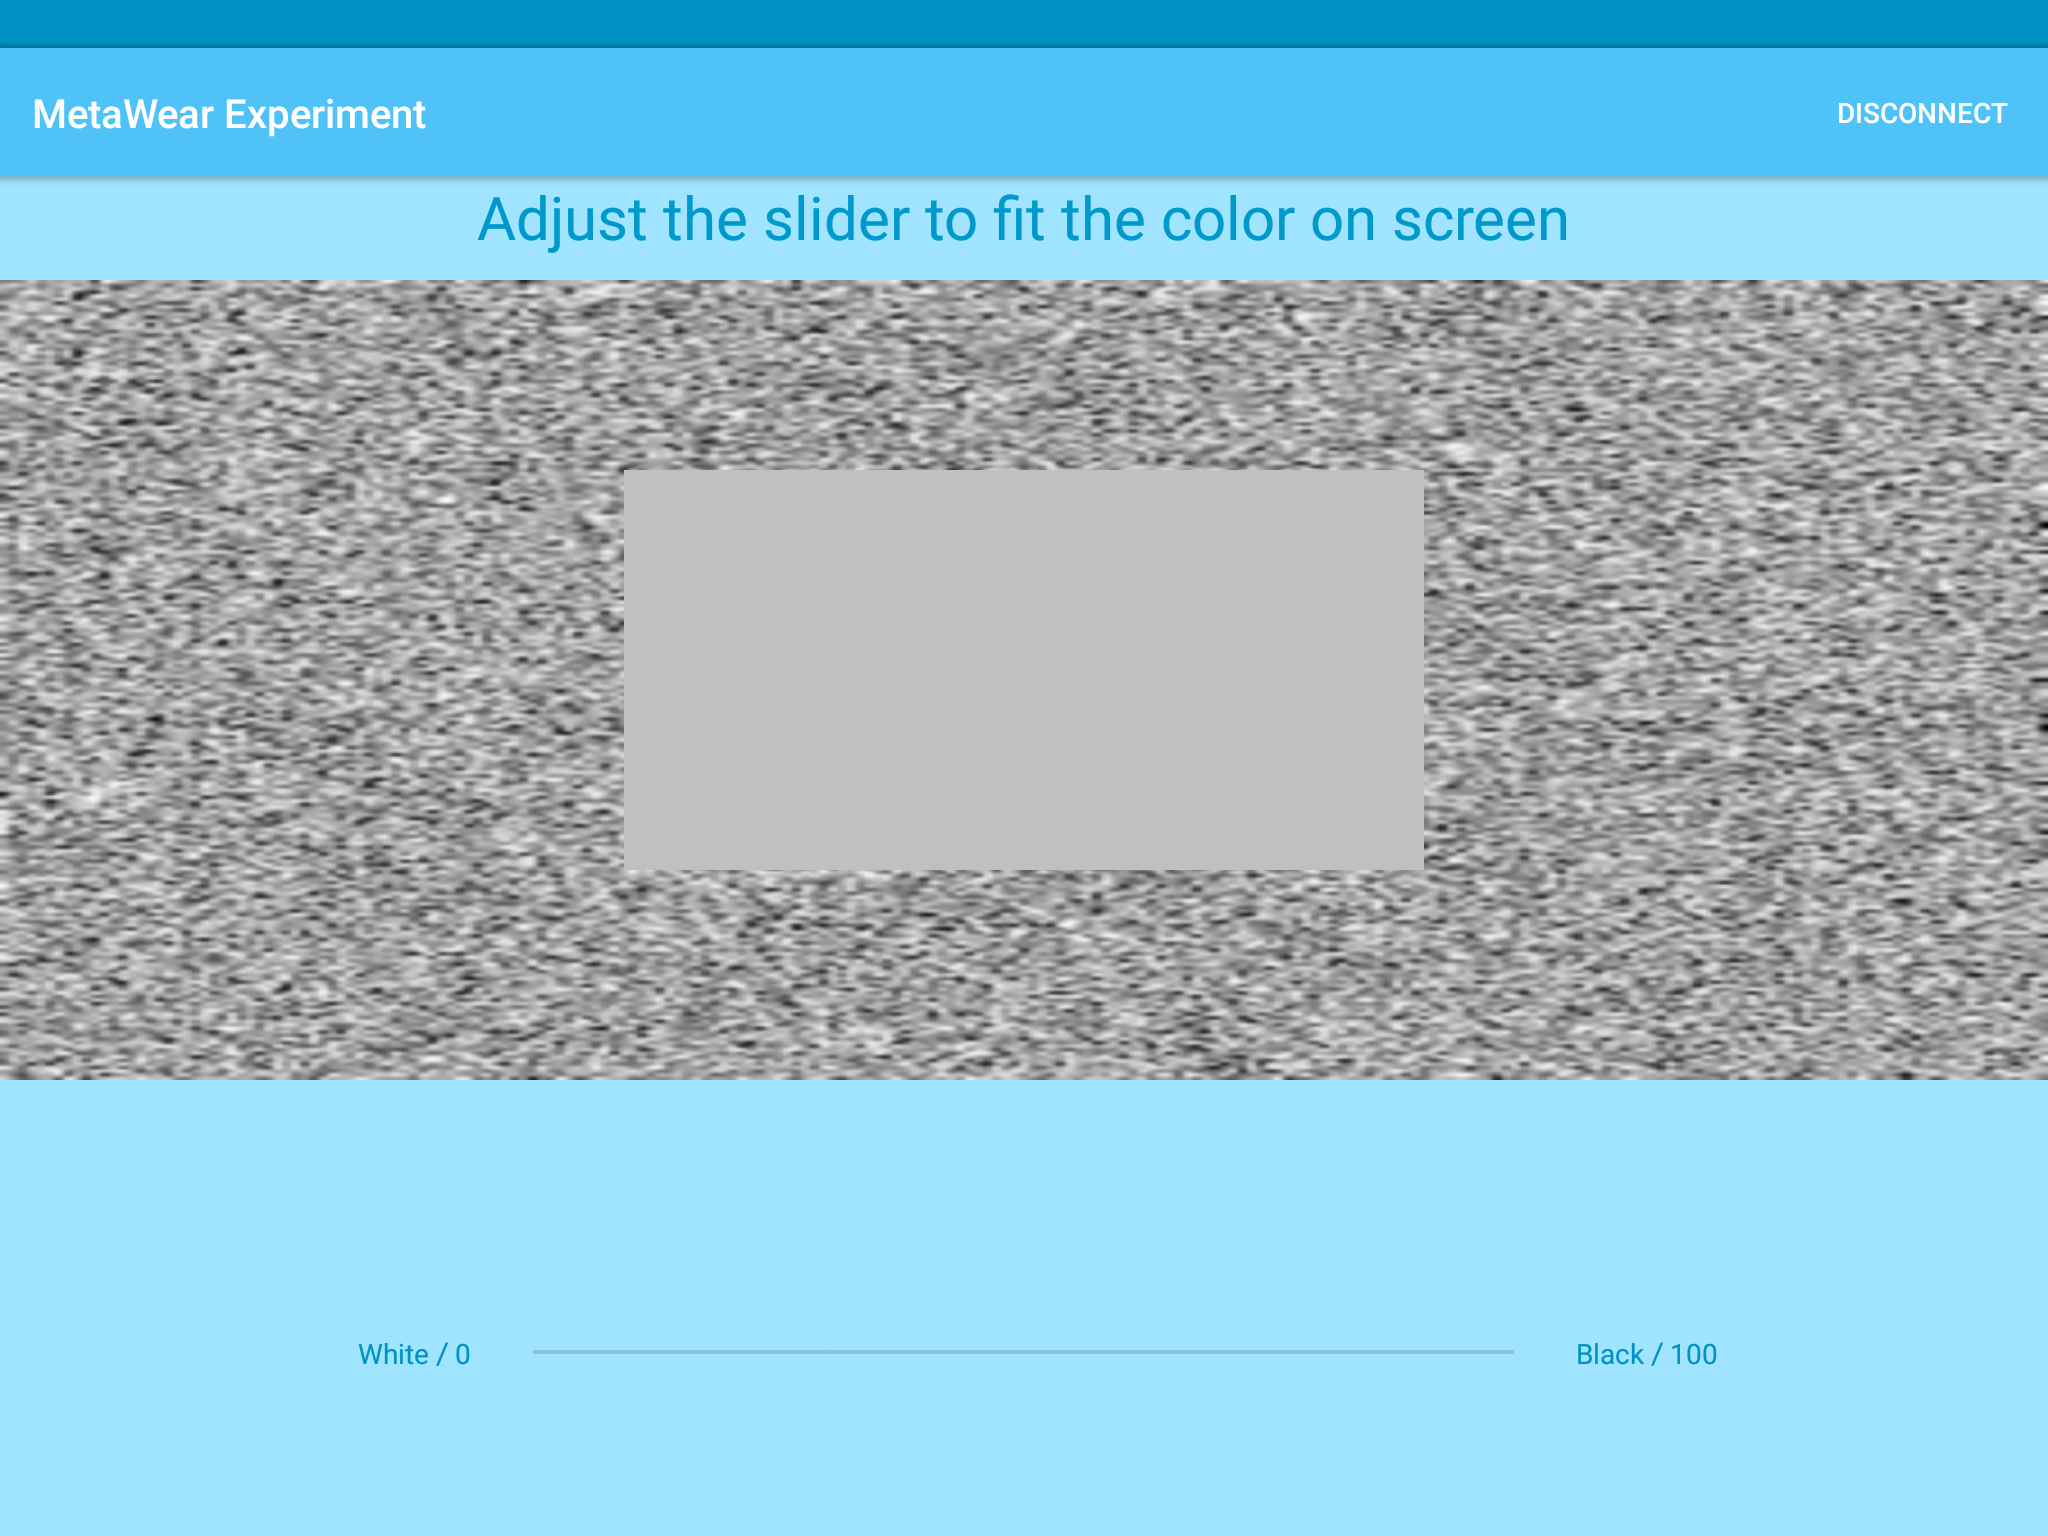
\includegraphics[width=0.95\linewidth]{figures/tablet_screen7.png}
  \captionof{figure}{Show stimuli screen with shade of grey}
  \label{app_show_stim}
\end{minipage}%
\begin{minipage}{.55\textwidth}
  \centering
  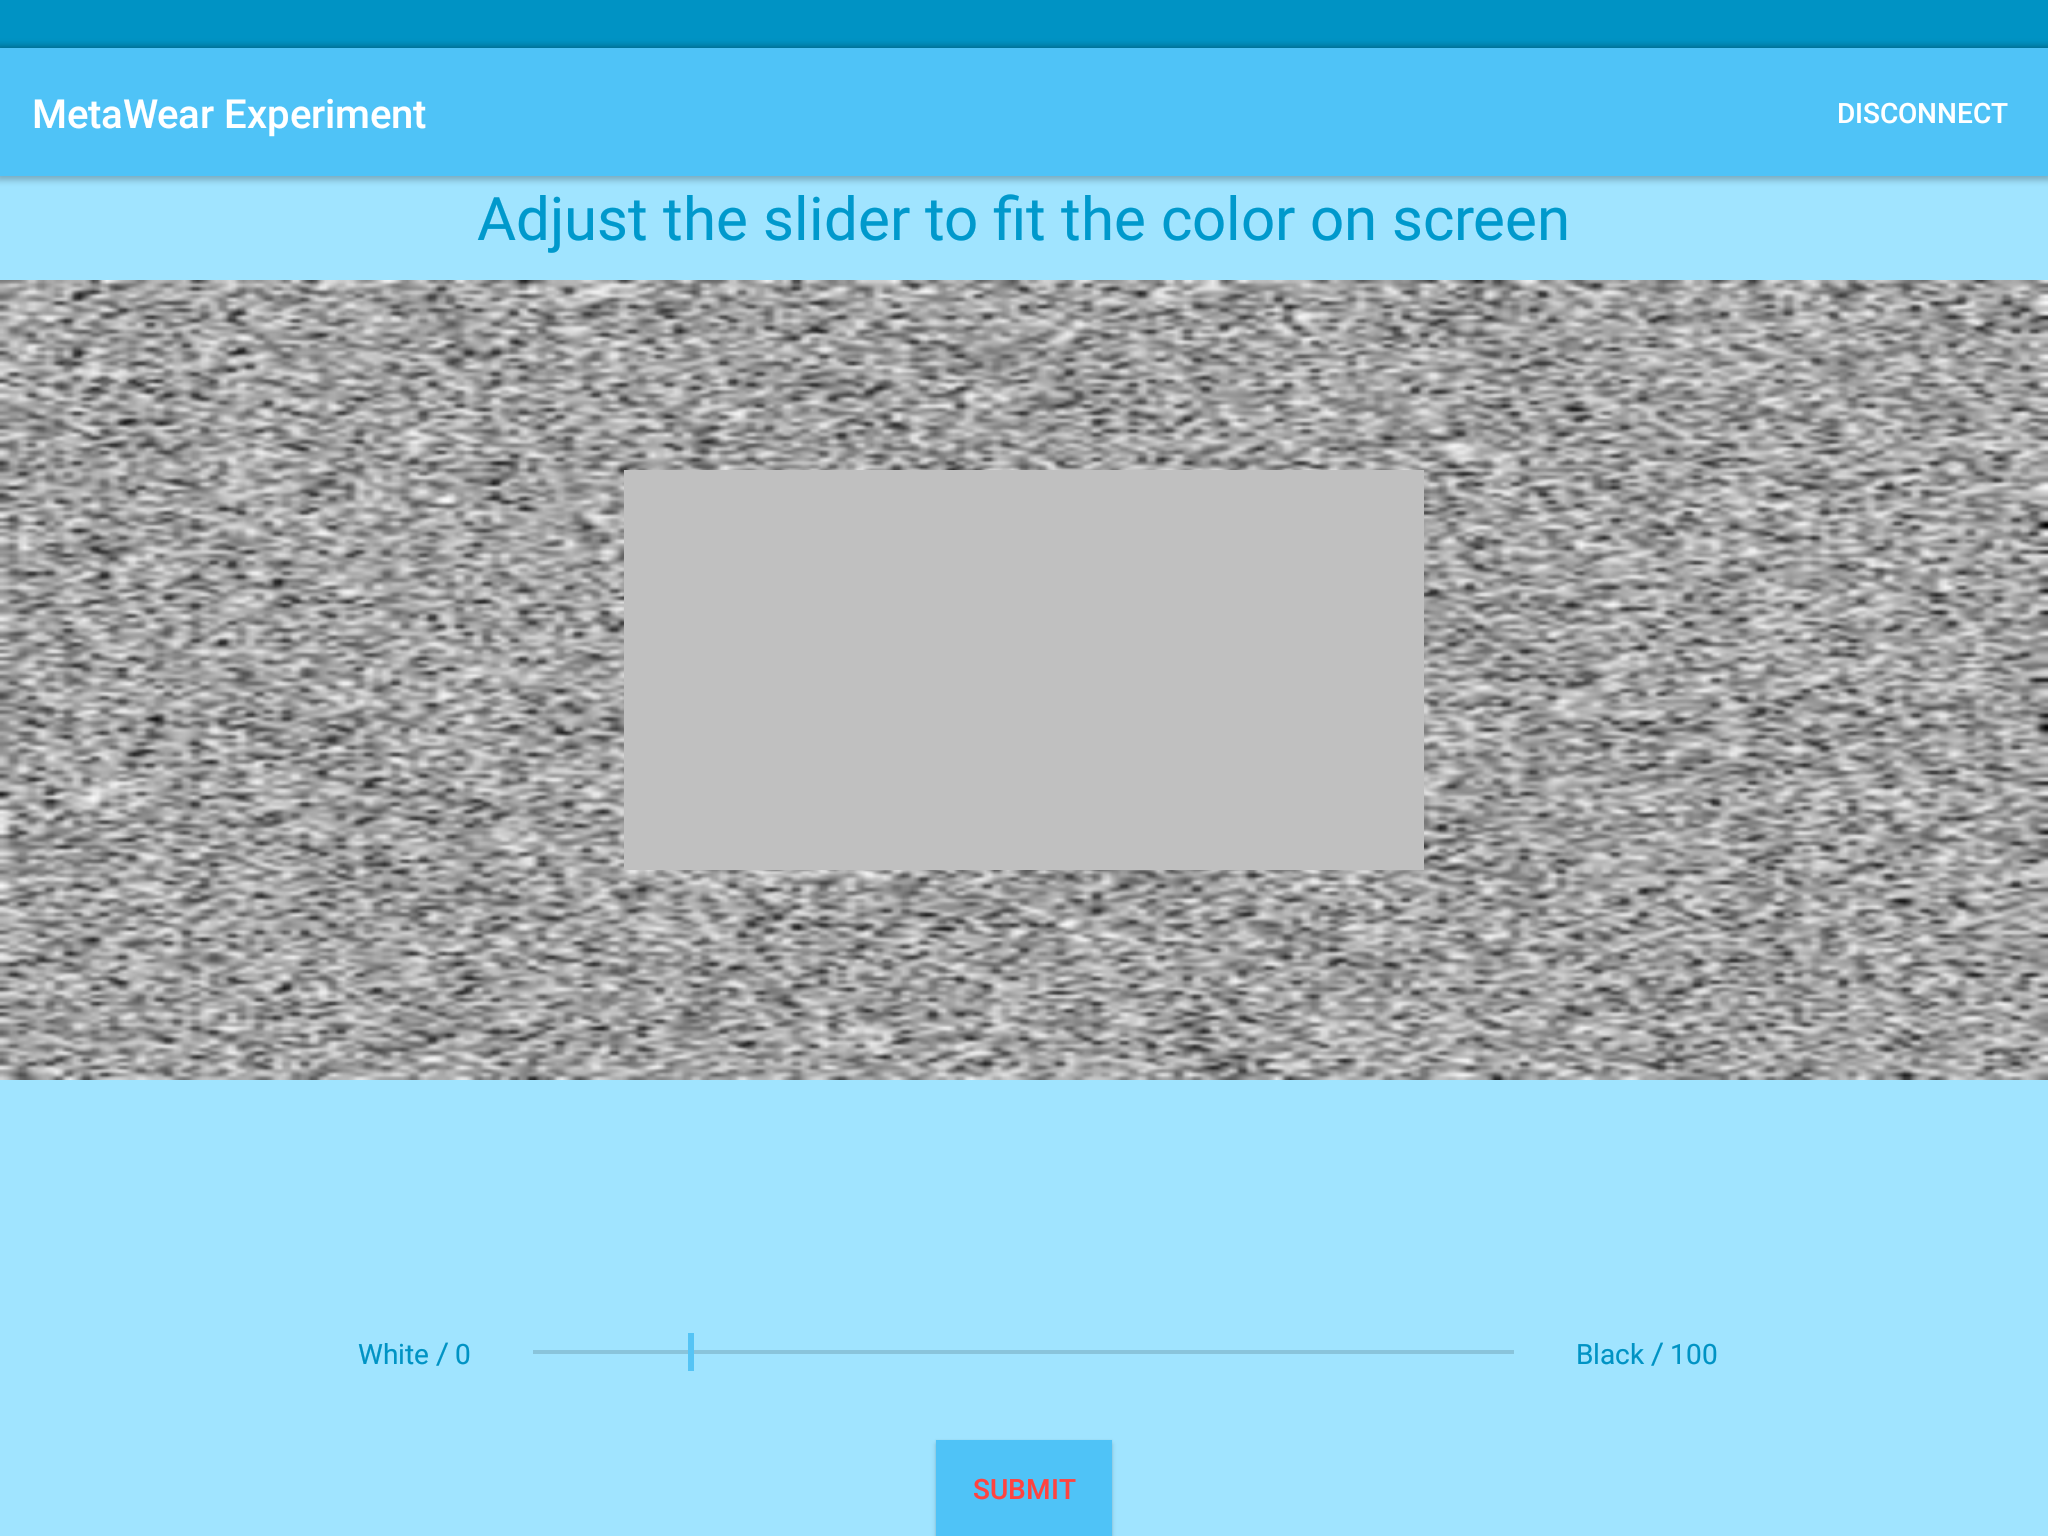
\includegraphics[width=0.95\linewidth]{figures/tablet_screen8.png}
  \captionof{figure}{Participant has given an input using the slider}
  \label{app_input_slider}
\end{minipage}
\end{figure}

\begin{figure}[h!]
\centering
\begin{minipage}{.55\textwidth}
  \centering
  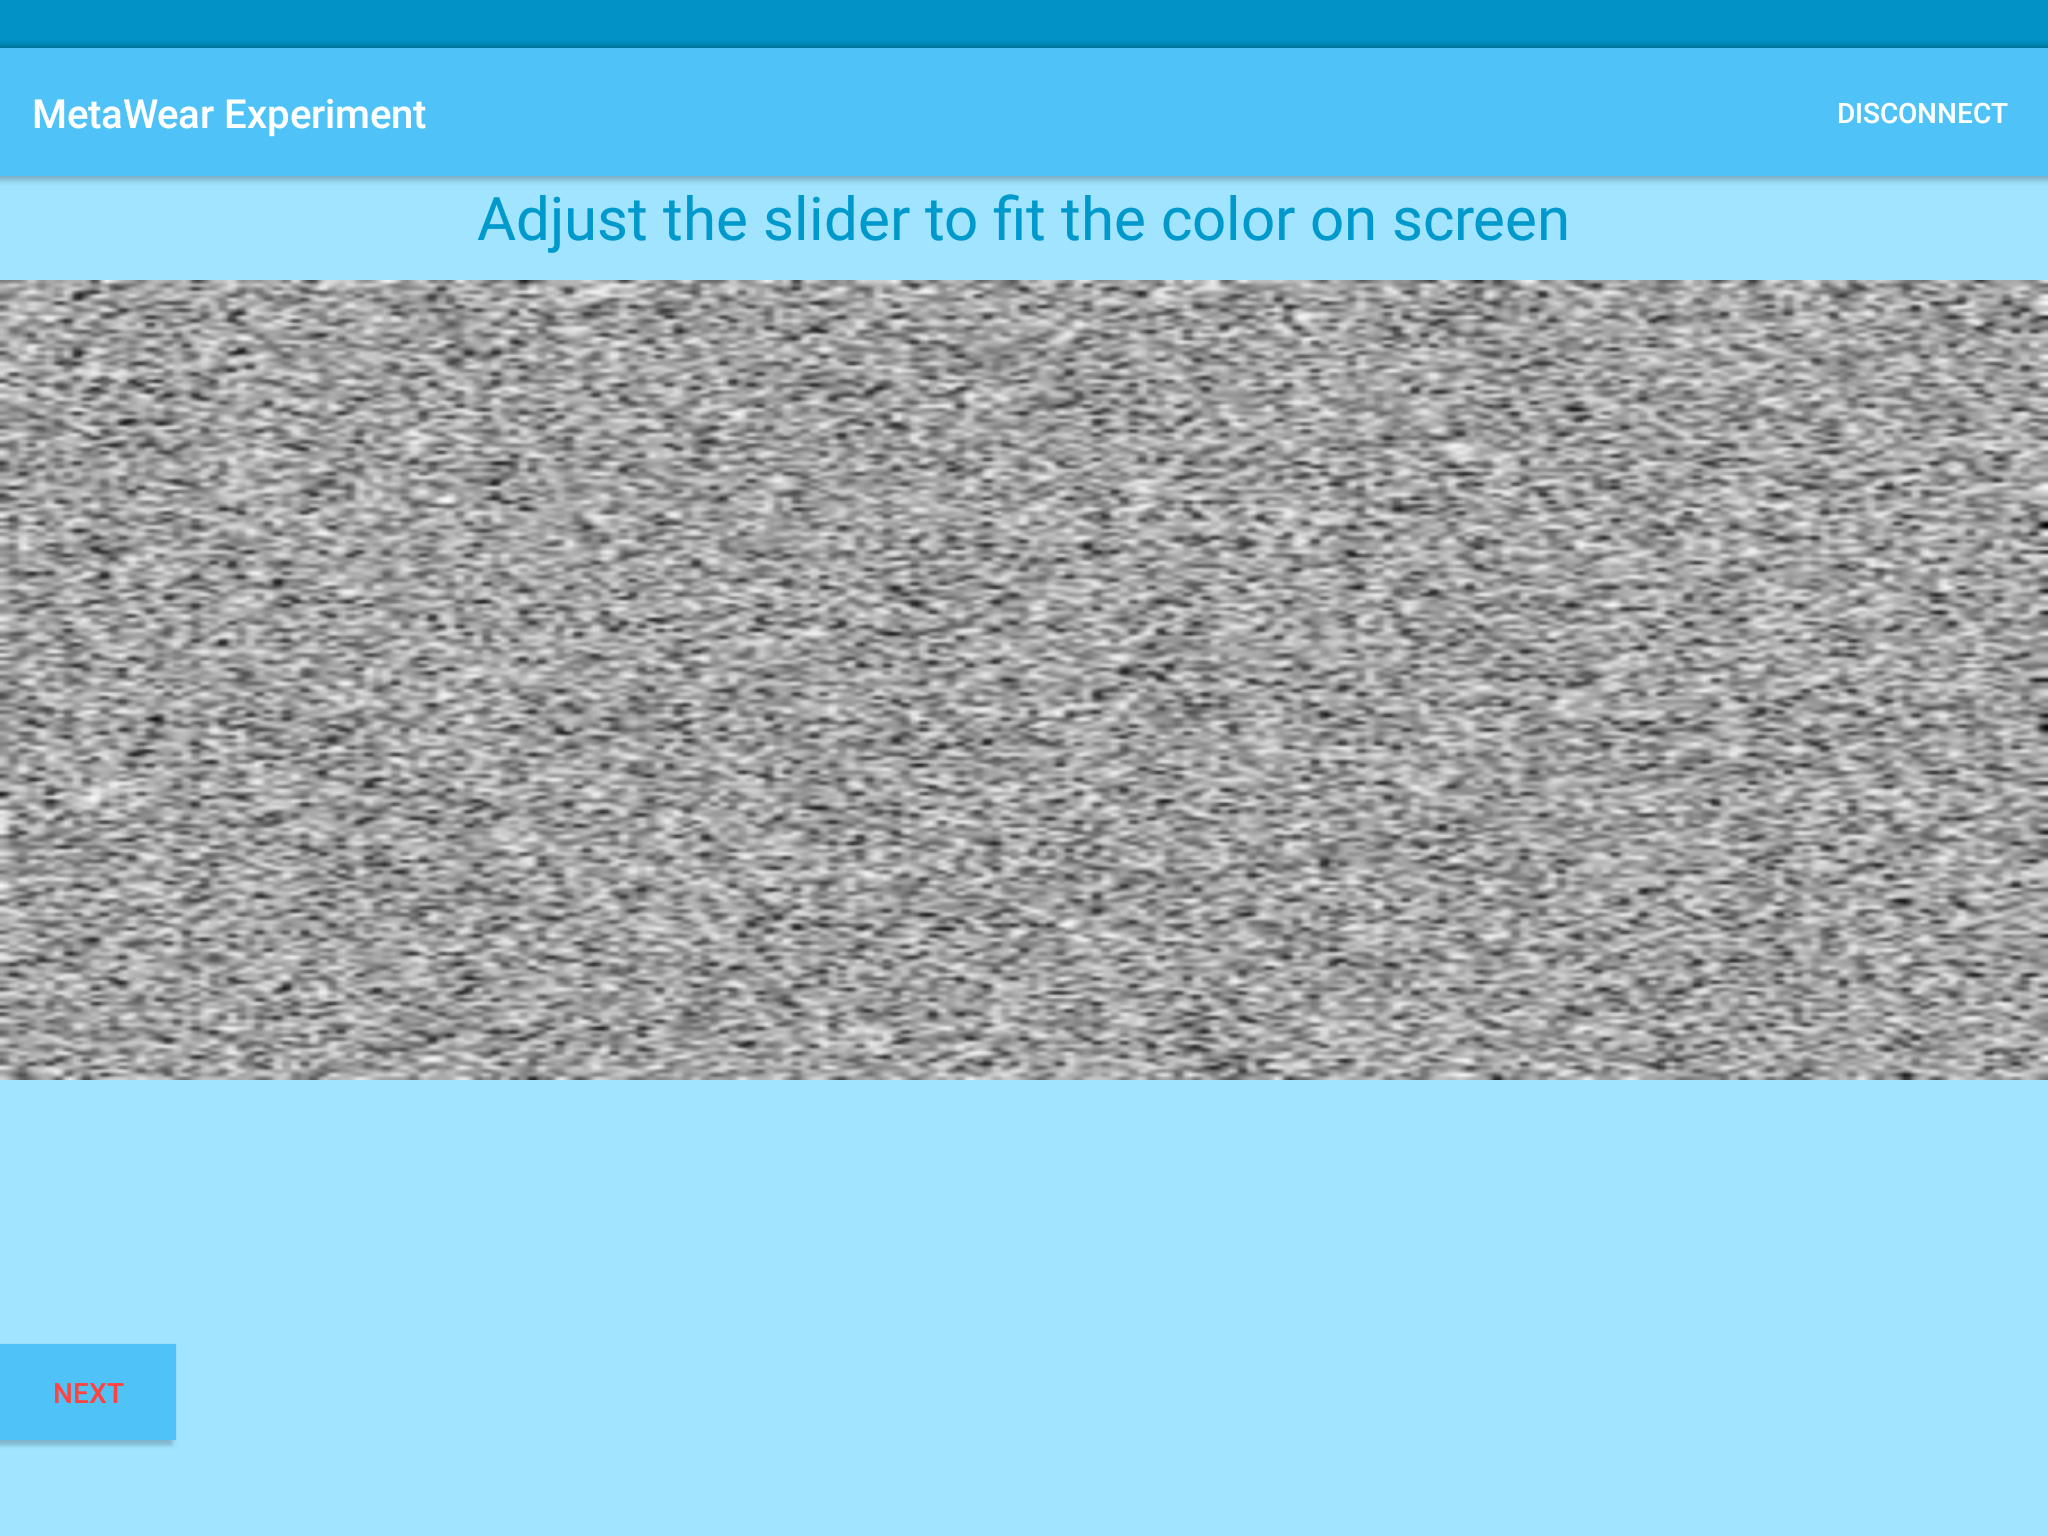
\includegraphics[width=0.95\linewidth]{figures/tablet_screen9.png}
  \captionof{figure}{Next stimuli screen}
  \label{app_next_stim}
\end{minipage}%
\begin{minipage}{.55\textwidth}
  \centering
  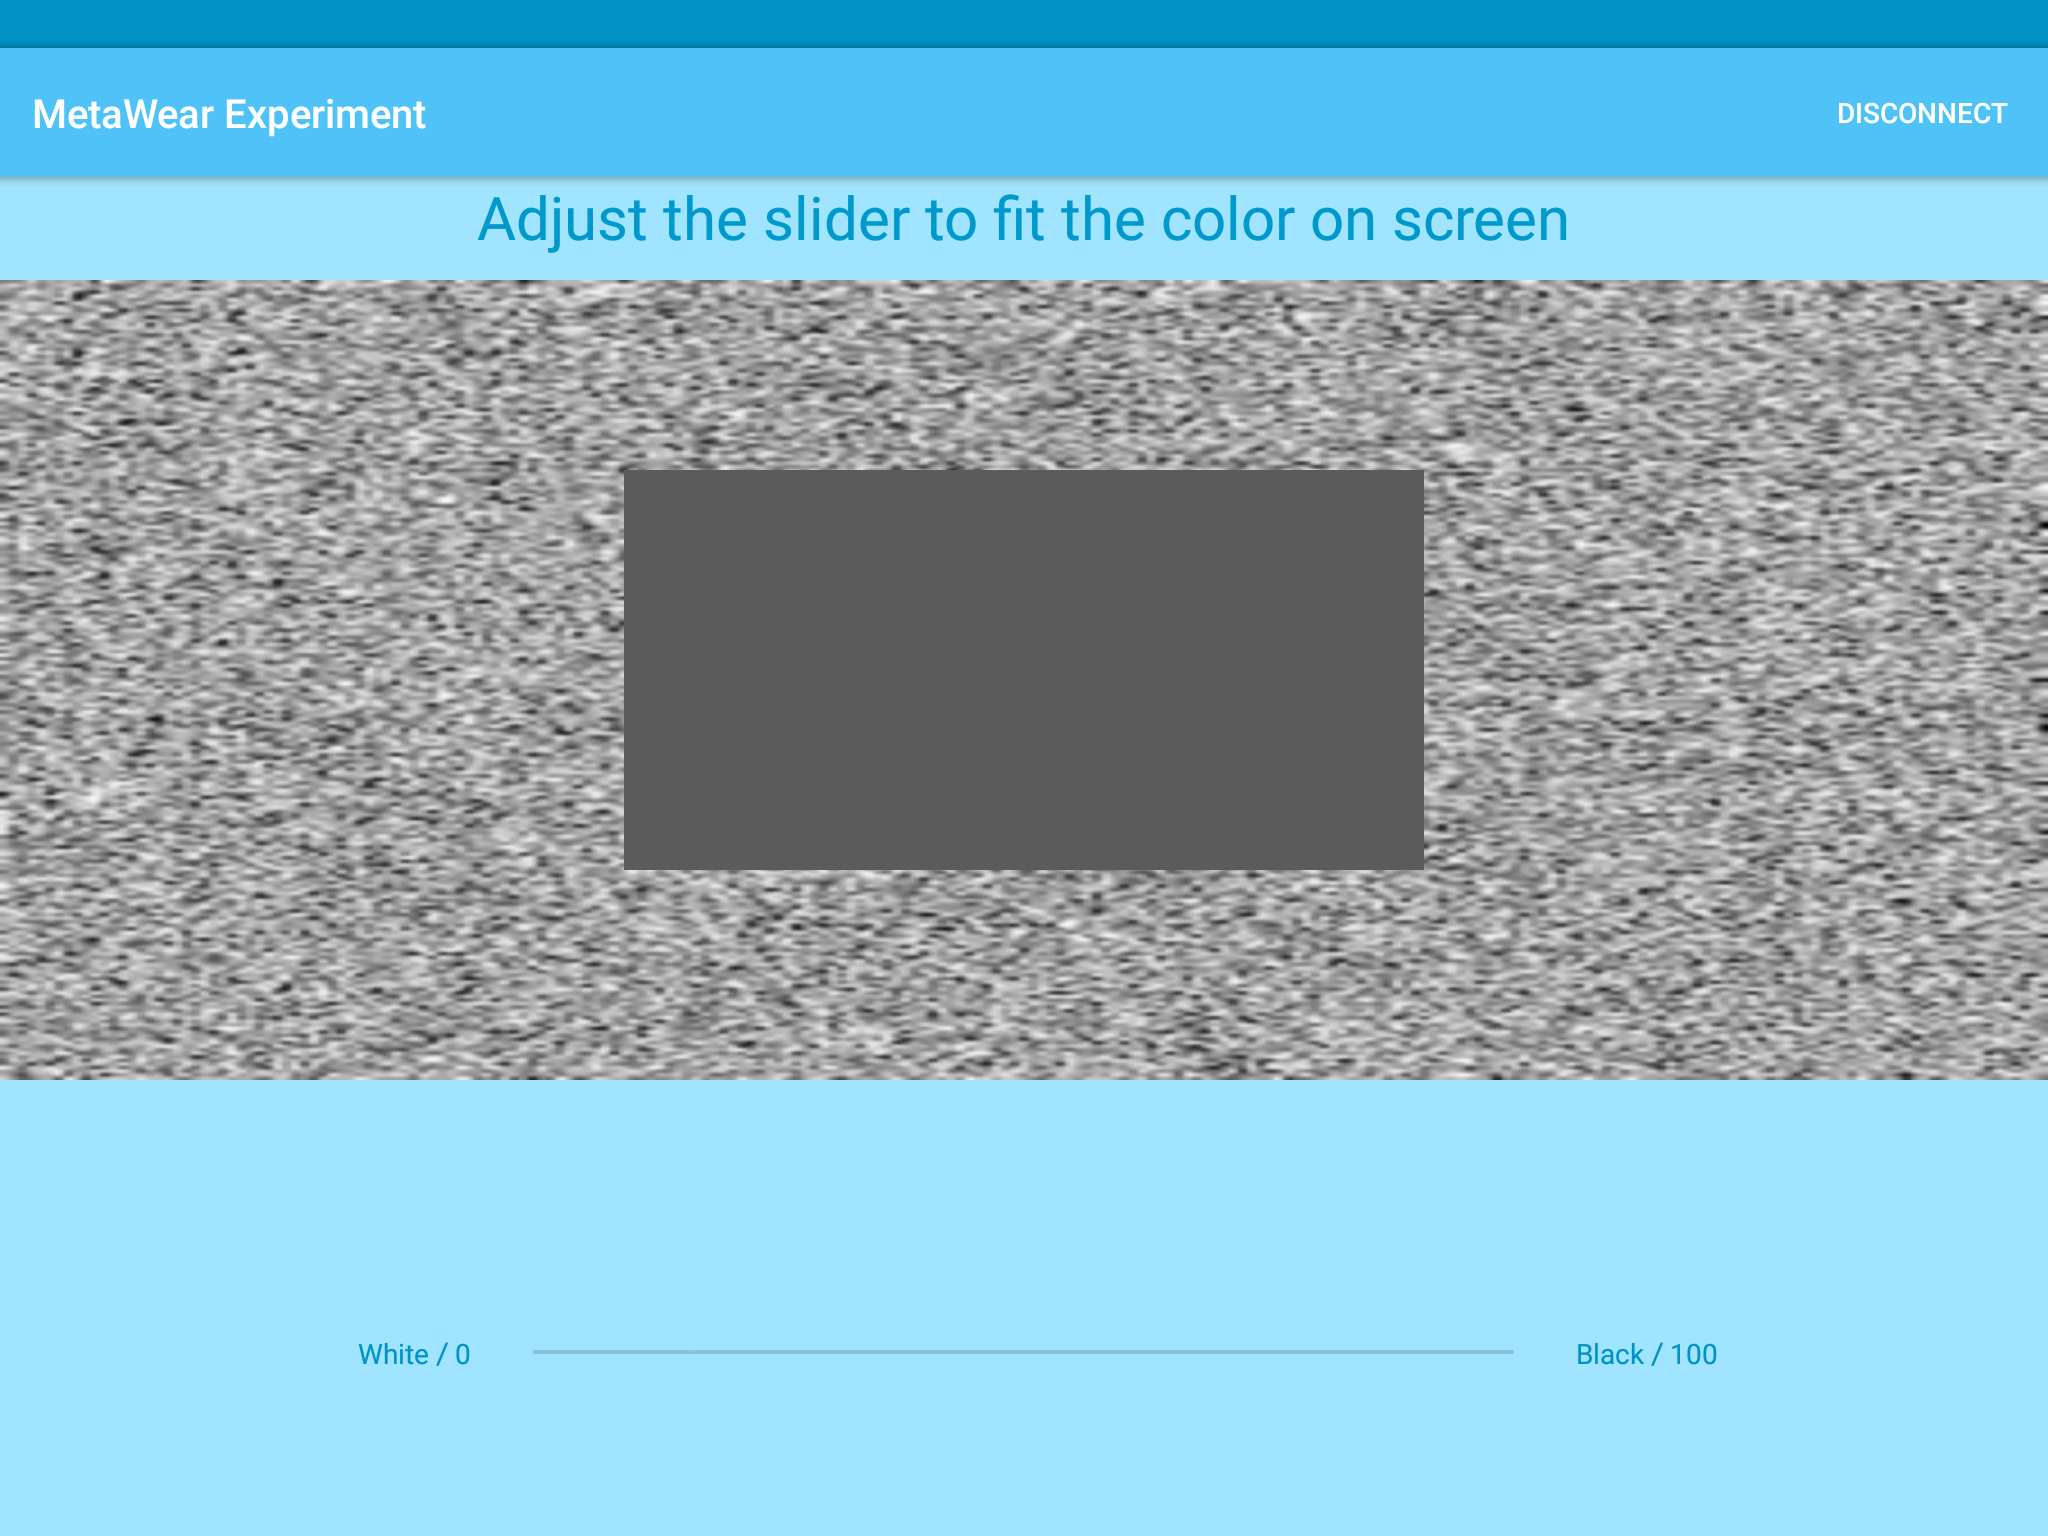
\includegraphics[width=0.95\linewidth]{figures/tablet_screen10.png}
  \captionof{figure}{Pattern is repeated}
  \label{app_repeat}
\end{minipage}
\end{figure}

\begin{figure}[h!]
\centering
\begin{minipage}{.55\textwidth}
  \centering
  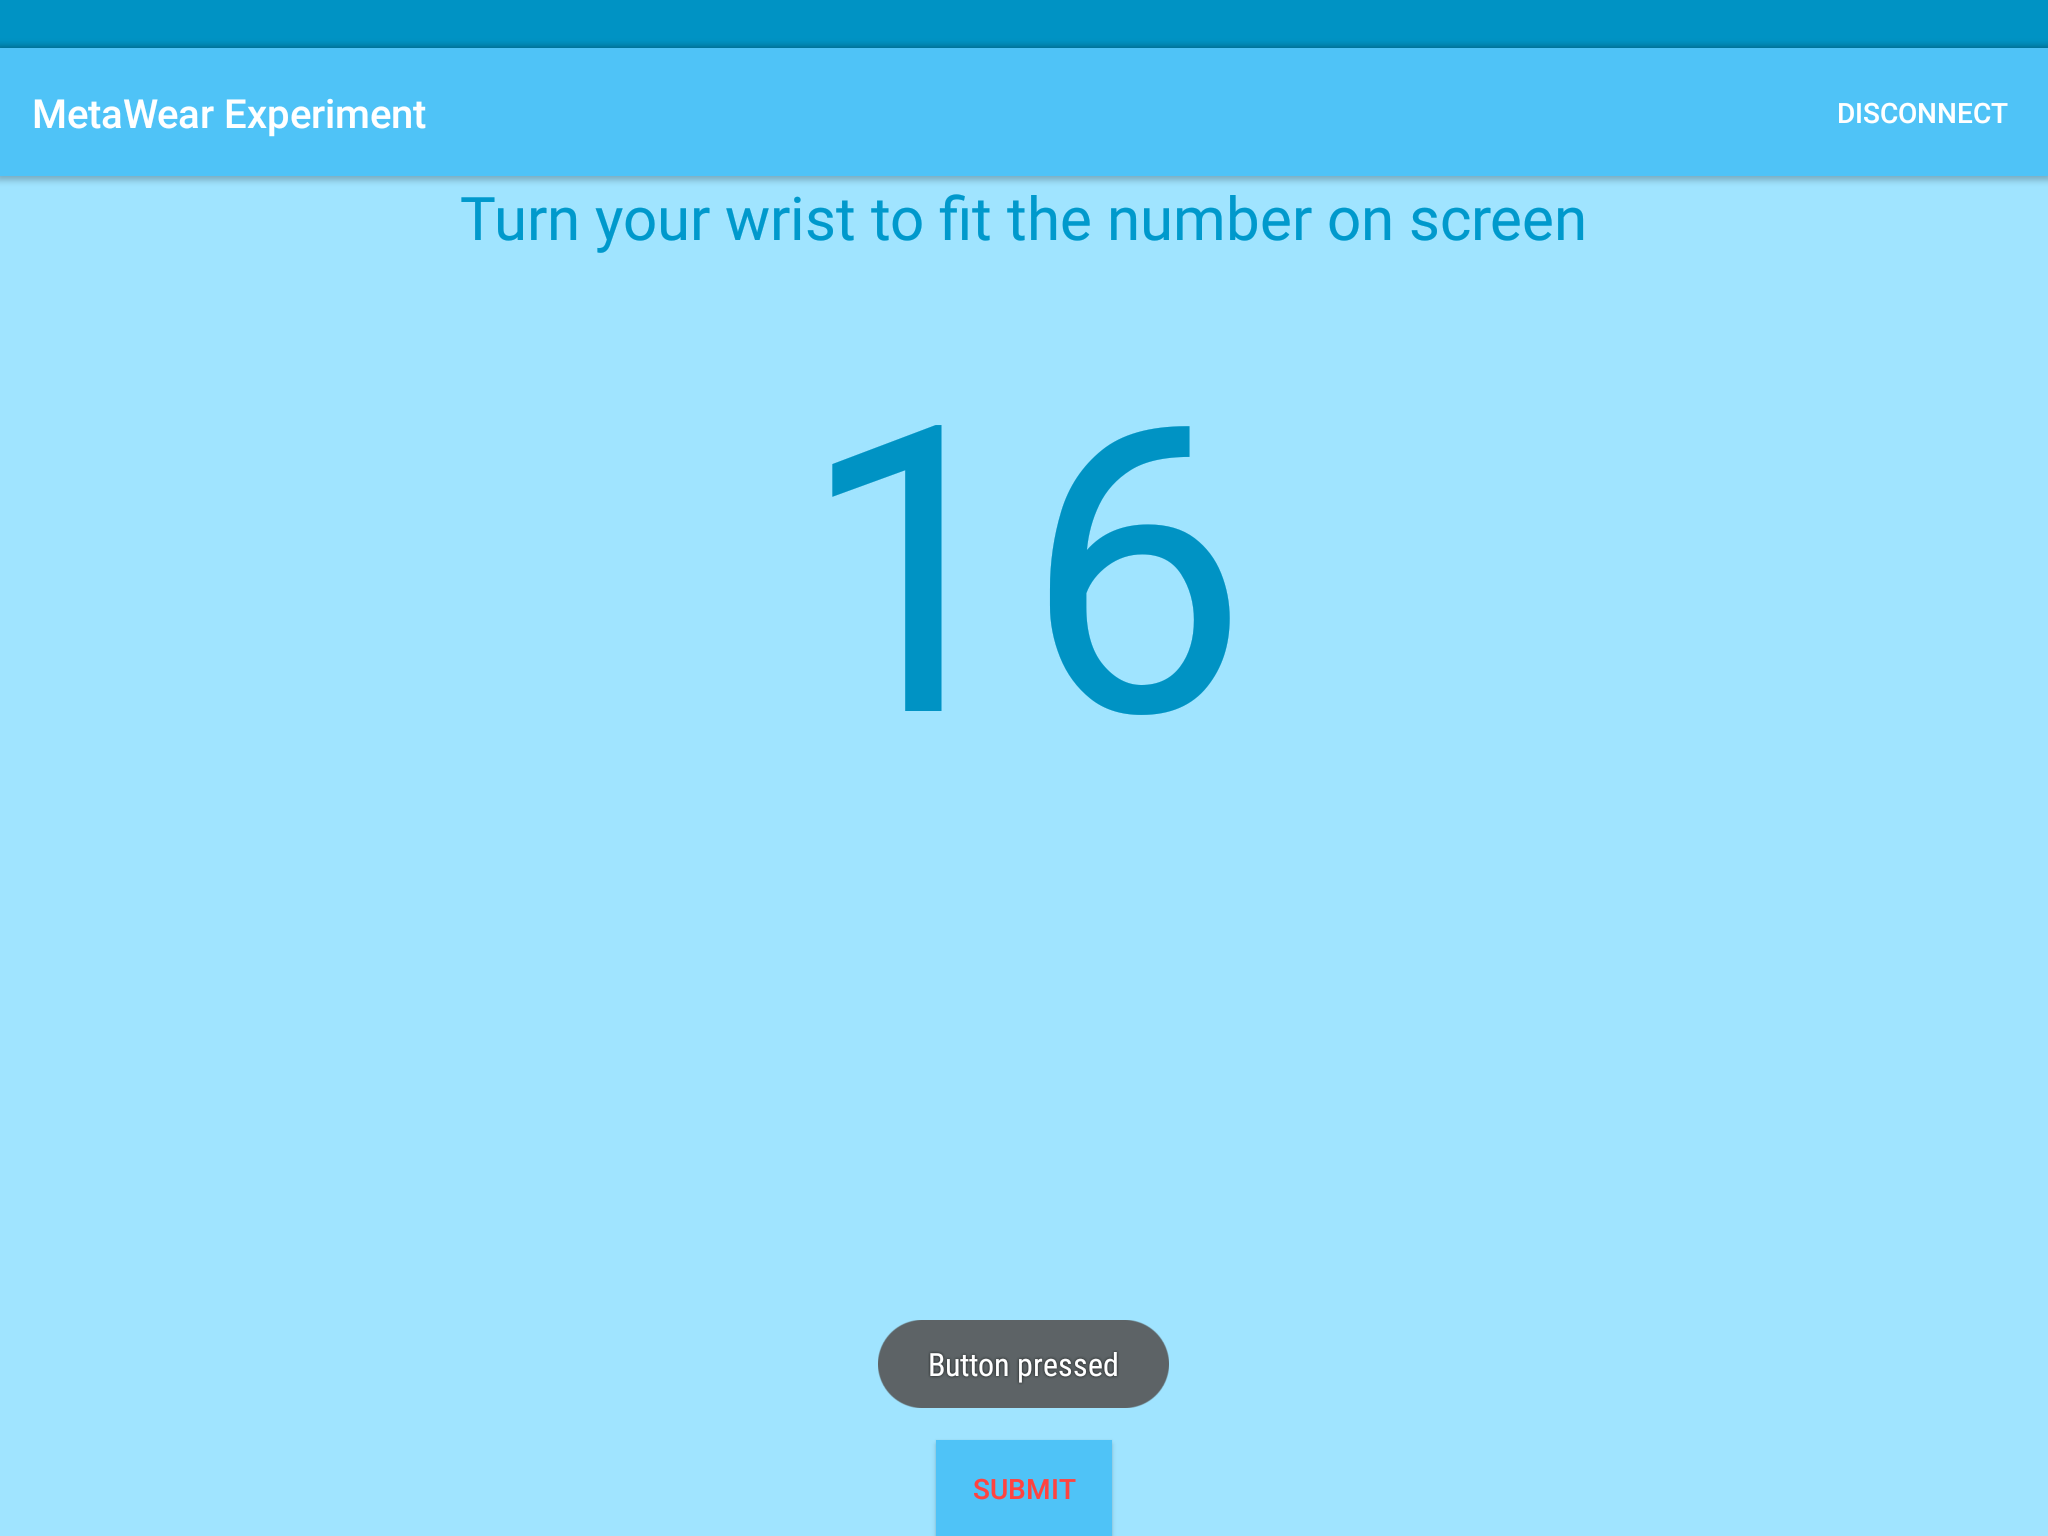
\includegraphics[width=0.95\linewidth]{figures/tablet_screen16.png}
  \captionof{figure}{Input registered from wristband with integer stimuli}
  \label{app_wrist_int}
\end{minipage}%
\begin{minipage}{.55\textwidth}
  \centering
  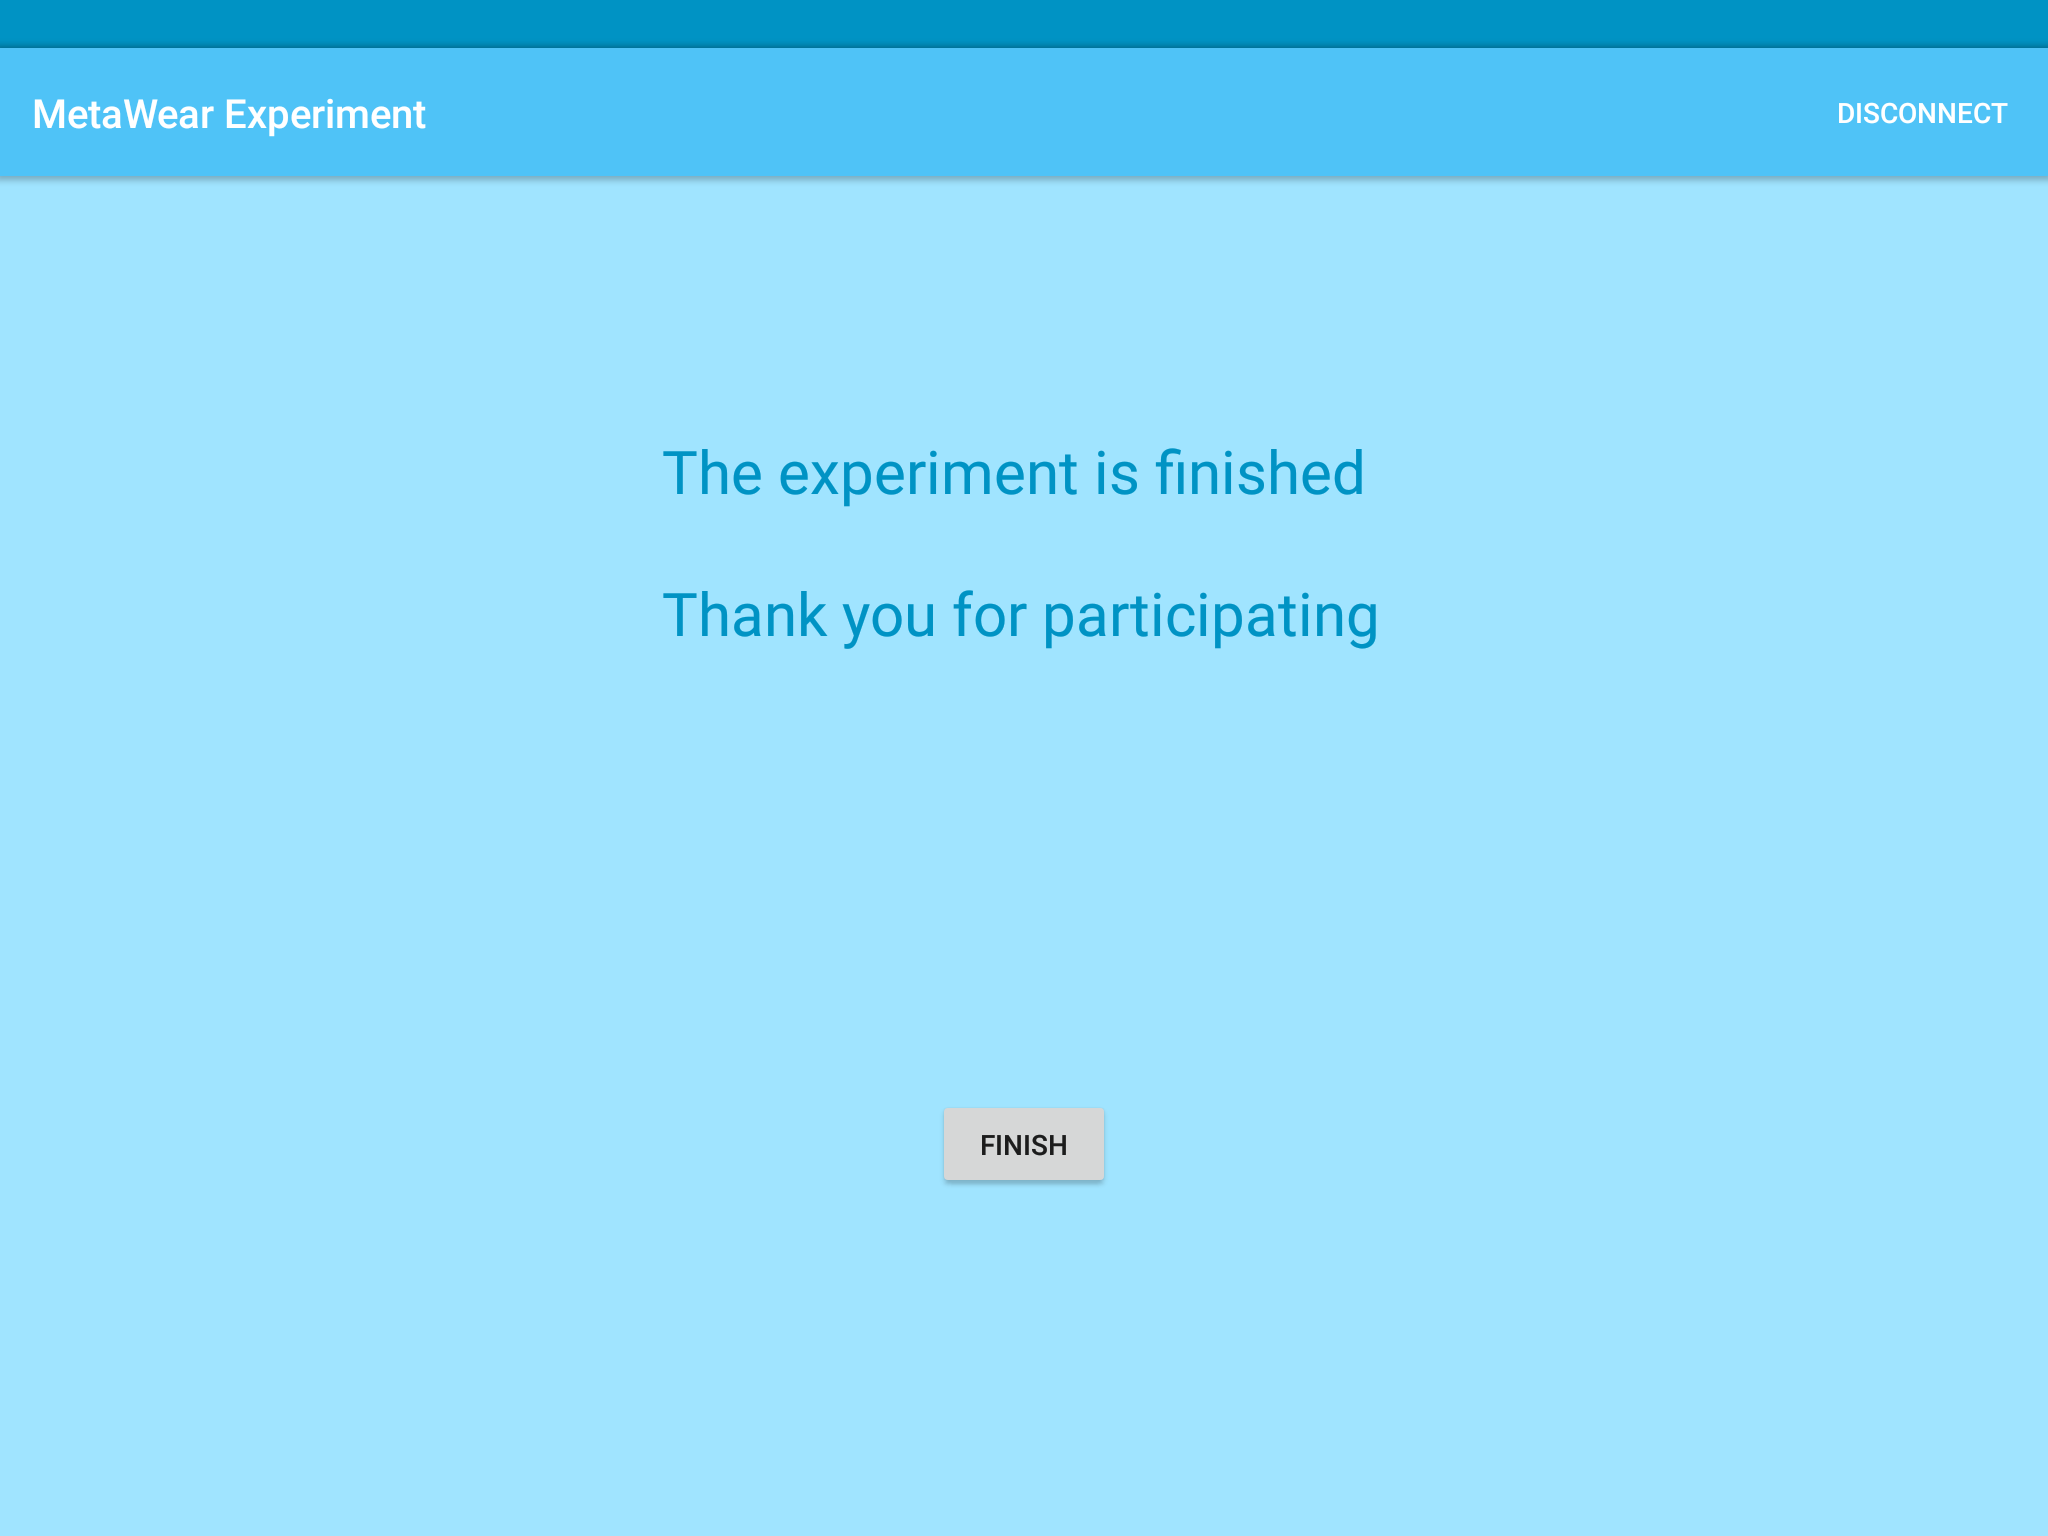
\includegraphics[width=0.95\linewidth]{figures/tablet_screen17.png}
  \captionof{figure}{Finished experiment screen}
  \label{app_finish}
\end{minipage}
\end{figure}

The stimuli for each exercise follow a specific set of rules. First of all the stimuli for each exercise is independent. For num exercises the stimuli is generated by creating an array of integers from 0-100, e.g. [0, 1, 2 .. 98, 99, 100]. This array is shuffled so the order is random. When a stimuli is needed the first element in the array is used, once used it is removed from the array. Once the array is empty the process is repeated. For grey exercises the process is the same, but the array consist of integers from 0-49, here 0 correspond to pure white, 49 is pure black and the rest are the shaded of grey in between. The shaded of grey are the same as used by Matejka et al.\cite{grey} as seen in Figure \ref{50shades}, where each shade is of equal distance from each other in the CIELAB color space\cite{cielab}. What this means is that the order of stimuli is completely random, but the distribution of stimuli is completely even, this means that for each participant the stimuli is random but not repeated, while keeping the overall even distribution between participants. Again emphasizing on the fact that the stimuli for each exercise is independent.

The data collected from the experiment is described in Table \ref{data_in}. Data is recorded whenever the participant pressed the submit button for each trial. With the six exercises each having 20 trials, this results in 120 data points for each participant and a total of 2880 data points for the complete experiment. Most of the data is self explanatory and doesn't need further explanation than the table. The \say{type} refers to the exercise. \say{type\_order} refers to the order of the exercises, this data is redundant since it can be deducted based on the \say{id} and Table \ref{latin}. \say{stim\_order} is the order the stimuli had and is also redundant since it can be deducted based on the time stamp, but if any of these were to be investigated this would greatly reduce the work. The \say{pitch}, \say{roll} and \say{yaw} are the Euler angles recorded, these could be used to change the mapping functions from Euler angles to scaled value without needing to redo experiment (these values are only recorded for wrist and arm exercises). The \say{reaction\_time} is recorded from when the stimuli was shown on screen until the participant pressed the submit button. The data collected is saved to a CSV file in the apps internal storage, and can be exported from the settings screen as described earlier. Beside this data, a separate data file was created where to total time taken to complete the experiment (from pressing start in Figugre \ref{app_ex_start} to the finsih screen was shown).


% Please add the following required packages to your document preamble:
% \usepackage{graphicx}
\begin{table}[h!]
\centering
\resizebox{\textwidth}{!}{%
\begin{tabular}{lll}
column name                          & type                                  & descriptiom                                                                                                                                                            \\ \hline
\multicolumn{1}{|l|}{id}             & \multicolumn{1}{l|}{int}              & \multicolumn{1}{l|}{Uniqe id for each particpant}                                                                                                                      \\ \hline
\multicolumn{1}{|l|}{gender}         & \multicolumn{1}{l|}{String}           & \multicolumn{1}{l|}{Participant gender: "Male" or "Female"**}                                                                                                          \\ \hline
\multicolumn{1}{|l|}{age}            & \multicolumn{1}{l|}{int}              & \multicolumn{1}{l|}{Participant age**}                                                                                                                                 \\ \hline
\multicolumn{1}{|l|}{time}           & \multicolumn{1}{l|}{Date object}      & \multicolumn{1}{l|}{Timestamp when input was registered}                                                                                                               \\ \hline
\multicolumn{1}{|l|}{type}           & \multicolumn{1}{l|}{String}           & \multicolumn{1}{l|}{\begin{tabular}[c]{@{}l@{}}Type of exercise: "slider\_grey", "slider\_num", "wrist\_grey",\\ "wrist\_num", "arm\_grey" or "arm\_num"\end{tabular}} \\ \hline
\multicolumn{1}{|l|}{type\_order}    & \multicolumn{1}{l|}{int}              & \multicolumn{1}{l|}{Order for the type of exercise: 0-5*}                                                                                                              \\ \hline
\multicolumn{1}{|l|}{stim\_order}    & \multicolumn{1}{l|}{int}              & \multicolumn{1}{l|}{Order for the stimuli: 0-49 or 0-100*}                                                                                                             \\ \hline
\multicolumn{1}{|l|}{stim}           & \multicolumn{1}{l|}{int}              & \multicolumn{1}{l|}{Stimuli: 0-49 or 0-100}                                                                                                                            \\ \hline
\multicolumn{1}{|l|}{response}       & \multicolumn{1}{l|}{double}           & \multicolumn{1}{l|}{Response: 0.0-49.0 or 0.0-100.0}                                                                                                                   \\ \hline
\multicolumn{1}{|l|}{pitch}          & \multicolumn{1}{l|}{double or String} & \multicolumn{1}{l|}{Value of pitch for exercises using the wristband, else "NA"**}                                                                                     \\ \hline
\multicolumn{1}{|l|}{roll}           & \multicolumn{1}{l|}{double or String} & \multicolumn{1}{l|}{Value of roll for exercises using the wristband, else "NA"**}                                                                                      \\ \hline
\multicolumn{1}{|l|}{yaw}            & \multicolumn{1}{l|}{double or String} & \multicolumn{1}{l|}{Value of yaw for exercises using the wristband, else "NA"**}                                                                                       \\ \hline
\multicolumn{1}{|l|}{reaction\_time} & \multicolumn{1}{l|}{long}             & \multicolumn{1}{l|}{\begin{tabular}[c]{@{}l@{}}Time in milliseconds from the stimuli was shown\\ until a response was registred\end{tabular}}                          \\ \hline
                                     &                                       & *Redundant data. **Data not investigated                                                                                                                              
\end{tabular}%
}
\caption{Structure of Collected Data}
\label{data_in}
\end{table}

\subsection{Other}
Beside the described hardware and software a small foam pad was used for the participant to place their elbow on, this reduced fatigue. A power bank was connected to the tablet to keep the it from running out of power and to keep the angle between the display and table at 15º, this reducing the glance in the display from the ceiling lights and gave a better viewing angle. 



% % % % % % % % % % % % % % % % % % % 
% PROCEDURE % PROCEDURE % PROCEDURE %
% % % % % % % % % % % % % % % % % % %
\section{Procedure}
Each participant completed the experiment in one continuous sitting, the whole process took approximately 15 minutes from the entered the room until they left. First participant was seated in front of the tablet and assisted to wear the wristband correctly. They were told to wear it on the arm the felt most comfortable with, but all participants choose their left arm. Then the participants was informed of how the device worked, they where shown the same gestures described in Figure \ref{pitch} and \ref{roll} (the gestured was performed on them, they weren't shown the Figures). It was made clear that the horizontal position would register as a minimum value, that the horizontal position would register a maximal value. They were instructed about how the scaled value would decrease if they performed the gesture beyond the vertical point.

They were then taken to the \say{Train} screen of the app, where they were given 1-2 minutes with each gesture to get a sense of the scale. They were asked to produce an input as close to zero and ten as possible. Again they were told about the what would happen if the went beyond the gesture, and they could see the result. They where then instructed to after each input with the wristband to lay their hand flat on the table. This was to have the same baseline for each input.

After training they were instructed on the structure of the experiment. They were told about the three input methods and two kinds of stimuli, and that there would be six exercises in total. They were told that each exercise would start with an explanation screen, then show a stimuli that they had to rate according to the instructions. They were told that each exercise had several stimuli, but they weren't told the exact amount, only that they had to continue the exercises until the saw the finish screen. They where told that if they where unhappy with an input, they could just press the button on the wristband again or adjust the slider before they pressed submit, but after pressing submit the input was final. Once they confirmed that they understood the instructions (any questions about the procedure was answered) they where taken to the experiment screen, where they registered their age and gender and then started the experiment. Most participants had no problems following the on screen instructions, but some participants asked questions during the experiment to clarify the task they had to perform. 

After completing the experiment they were handed the survey (Appendix \ref{survey}) on a computer and asked to answer it.

% % % % % % % % % % % % % % % % % % % %
% Design % Design % Design %  Design %
% % % % % % % % % % % % % % % % % % % %
\subsection{Design}


Within-subject: less people, variance due to participants’ predispositions will be approximately the same across test conditions.

Balanced Latin Square


% Please add the following required packages to your document preamble:
% \usepackage{graphicx}
\begin{table}[]
\centering
\resizebox{\textwidth}{!}{%
\begin{tabular}{rcccccc}
\cline{2-7}
\multicolumn{1}{r|}{Exercise} & \multicolumn{1}{l|}{slider\_grey} & \multicolumn{1}{l|}{slider\_num} & \multicolumn{1}{l|}{wrist\_grey} & \multicolumn{1}{l|}{wrist\_num} & \multicolumn{1}{l|}{arm\_grey} & \multicolumn{1}{l|}{arm\_num} \\ \cline{2-7} 
\multicolumn{1}{r|}{ID} & \multicolumn{1}{l|}{0} & \multicolumn{1}{l|}{1} & \multicolumn{1}{l|}{2} & \multicolumn{1}{l|}{3} & \multicolumn{1}{l|}{4} & \multicolumn{1}{l|}{5} \\ \cline{2-7} 
\multicolumn{1}{l}{} &  & \multicolumn{1}{l}{} & \multicolumn{1}{l}{} & \multicolumn{1}{l}{} & \multicolumn{1}{l}{} & \multicolumn{1}{l}{} \\
 & \multicolumn{6}{c}{Exercise Order} \\
Participant id & First & Second & Third & Fourth & Fifth & Sixth \\ \cline{2-7} 
\multicolumn{1}{r|}{0, 6, 12, 18} & \multicolumn{1}{c|}{\textbf{0}} & \multicolumn{1}{c|}{\textbf{1}} & \multicolumn{1}{c|}{\textbf{5}} & \multicolumn{1}{c|}{\textbf{2}} & \multicolumn{1}{c|}{\textbf{4}} & \multicolumn{1}{c|}{\textbf{3}} \\ \cline{2-7} 
\multicolumn{1}{r|}{1, 7, 13, 17} & \multicolumn{1}{c|}{\textbf{1}} & \multicolumn{1}{c|}{\textbf{2}} & \multicolumn{1}{c|}{\textbf{0}} & \multicolumn{1}{c|}{\textbf{3}} & \multicolumn{1}{c|}{\textbf{5}} & \multicolumn{1}{c|}{\textbf{4}} \\ \cline{2-7} 
\multicolumn{1}{r|}{2, 8, 14, 20} & \multicolumn{1}{c|}{\textbf{2}} & \multicolumn{1}{c|}{\textbf{3}} & \multicolumn{1}{c|}{\textbf{1}} & \multicolumn{1}{c|}{\textbf{4}} & \multicolumn{1}{c|}{\textbf{0}} & \multicolumn{1}{c|}{\textbf{5}} \\ \cline{2-7} 
\multicolumn{1}{r|}{3, 9, 15, 21} & \multicolumn{1}{c|}{\textbf{3}} & \multicolumn{1}{c|}{\textbf{4}} & \multicolumn{1}{c|}{\textbf{2}} & \multicolumn{1}{c|}{\textbf{5}} & \multicolumn{1}{c|}{\textbf{1}} & \multicolumn{1}{c|}{\textbf{0}} \\ \cline{2-7} 
\multicolumn{1}{r|}{4, 10, 16, 22} & \multicolumn{1}{c|}{\textbf{4}} & \multicolumn{1}{c|}{\textbf{5}} & \multicolumn{1}{c|}{\textbf{3}} & \multicolumn{1}{c|}{\textbf{0}} & \multicolumn{1}{c|}{\textbf{2}} & \multicolumn{1}{c|}{\textbf{1}} \\ \cline{2-7} 
\multicolumn{1}{r|}{5, 11, 17, 23} & \multicolumn{1}{c|}{\textbf{5}} & \multicolumn{1}{c|}{\textbf{0}} & \multicolumn{1}{c|}{\textbf{4}} & \multicolumn{1}{c|}{\textbf{1}} & \multicolumn{1}{c|}{\textbf{3}} & \multicolumn{1}{c|}{\textbf{2}} \\ \cline{2-7} 
\end{tabular}%
}
\caption{Exercise ordering table based on a Balanced Latin Square}
\label{latin}
\end{table}









% % % % % % % % % % % % % % % % % % % % % 
% PILOT TEST % PILOT TEST % PILOT TEST %
% % % % % % % % % % % % % % % % % % % % %
\section{Pilot tests}
Recording the time to complete the experiment. (include the data).









\chapter{Results \& Discussion}

The data collected was described in the previous Chapter, in Figure \ref{date_snip} we see a small snippet of the actual data collected. The whole data set and code for analysis can be found in Appendix \ref{ex_data_appendix} and \ref{data_anal_code}. 

\begin{figure}[]
    \centering
    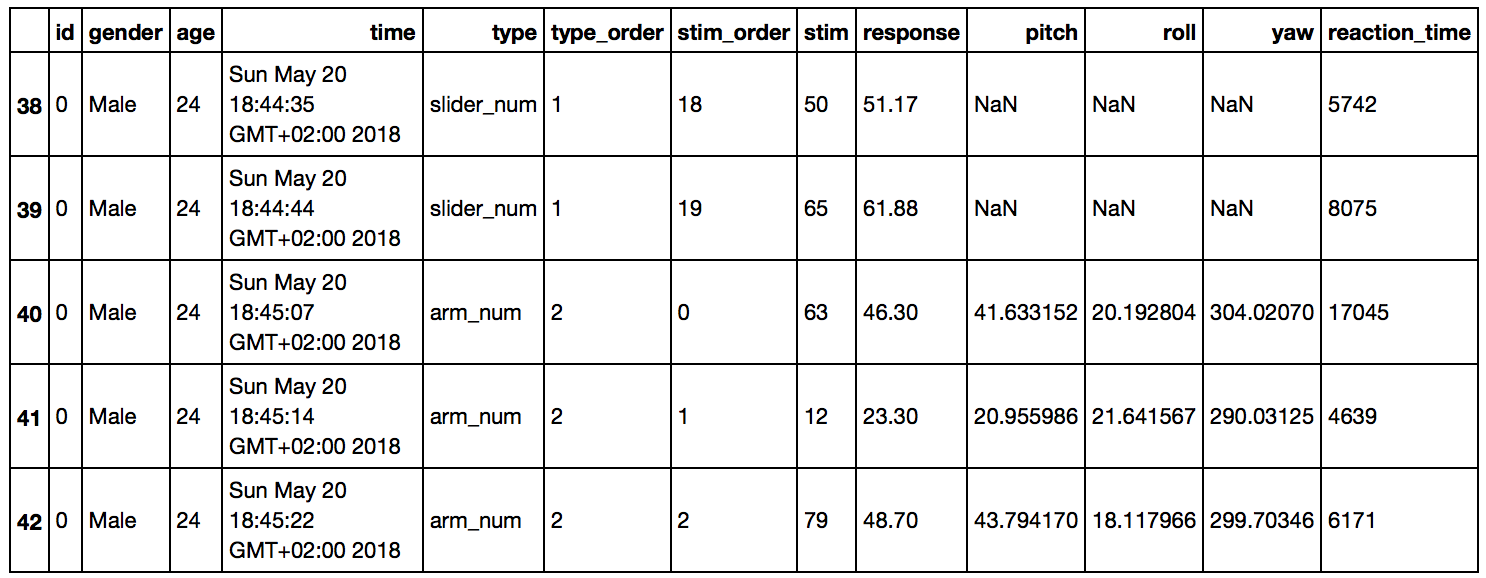
\includegraphics[width=1.2\textwidth]{figures/dataExample.png}
    \caption{Snippet of collected data}
    \label{data_snip}
\end{figure}

In the work of Matejka et al.\cite{grey} they define any response with an error greater than half the scale to an outlier, debating that an response this far from the stimuli must be seen as a human error. Using the same argument we will remove any data point where the difference between the stimuli and response was greater than half the scale. With the grey exercises 50 shades of greys where shown, with a corresponding value from 0 (pure white) to 49 (pure black), therefor we will remove any data point with a difference between stimuli and response that is more than 25. Likewise with the num exercises where the scale is from 0 to 100 any data point with a difference between the stimuli and response greater than 50 is removed. This results in the removal of four data points, which can be seen in Figure \ref{outliers}. 

\begin{figure}[]
    \centering
    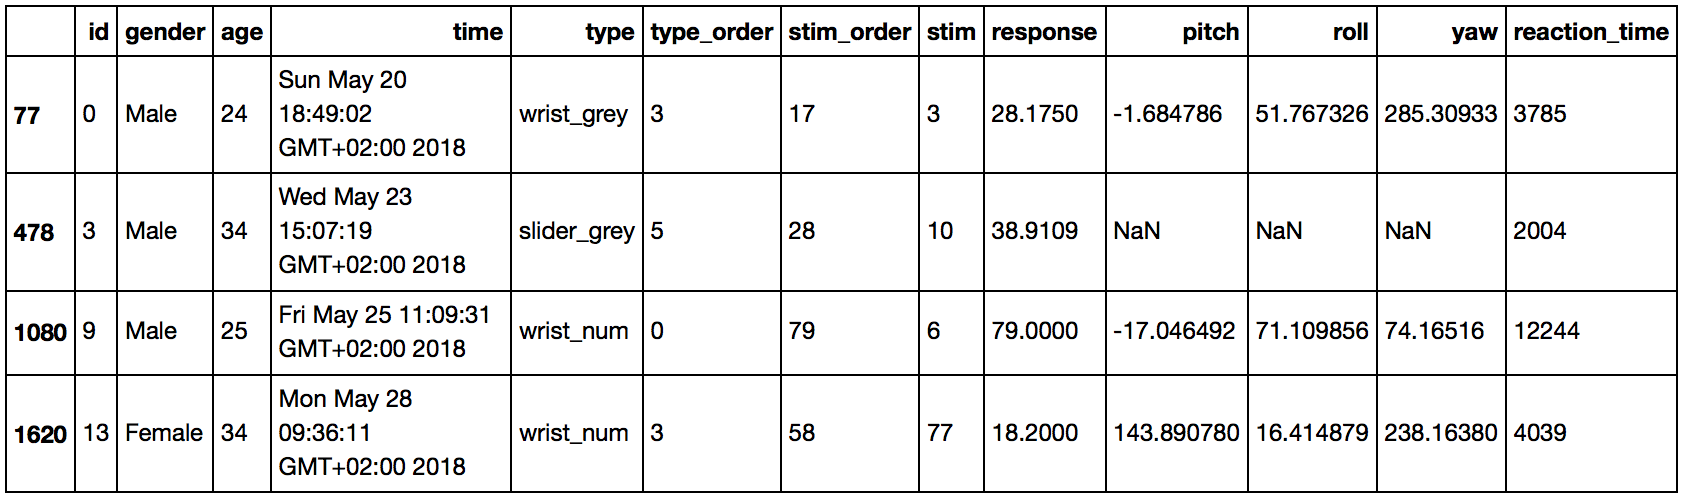
\includegraphics[width=1.2\textwidth]{figures/outliers.png}
    \caption{Removed outliers}
    \label{outliers}
\end{figure}

It seems reasonable to remove these four data points, but another approach is visual inspection of the data. This can be done by plotting each participants response over stimuli for each exercise, in Figure \ref{visual_out} we the result of this for the slider\_grey exercise, the plot has been divided into four plots with six participants on each. It then becomes easy to see by looking at each line if a point should be considered an outlier. If a line is fairly straight, but a single point is way off it can be considered an outlier, but if a line is fluctuating a lot, then it is more likely that the participant just wasn't very consistent, and therefor the a point on that line can't be considered an outlier. If we look to the lower right plot in Figure \ref{visual_out} an follow the orange line, we see that it is fairly straight, with the one exception at about (28, 12), since this is a single point that is way out line, this could be considered an outlier that must be due to user error. While this method can be effective at removing outliers, it can't be known for curtain if these point in fact are outliers, therefor this method has been discarded. The plots for the other exercises can be found in Appendix \ref{plots_appendix}.

\begin{figure}[]
    \centering
    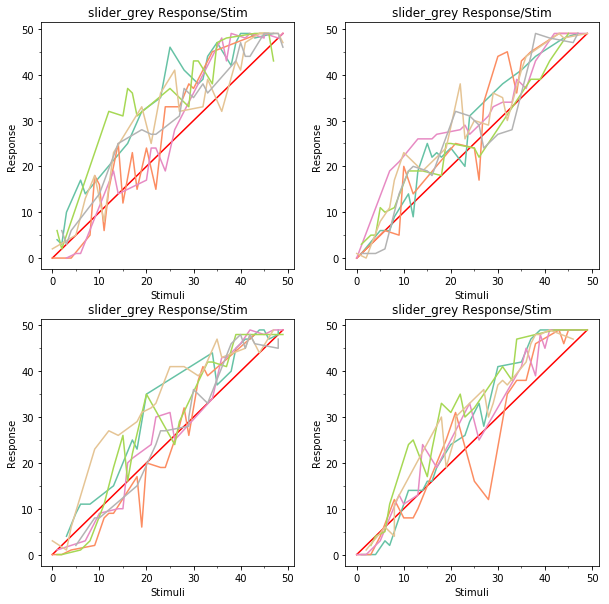
\includegraphics[width=0.75\textwidth]{figures/visual_out1.png}
    \caption{Visualization of outliers for the arm\_grey exercise. Each line correspond to the response from a single participant. The red diagonal would be a perfect response}
    \label{visual_out}
\end{figure}

In order to compare the wristband to the digital VAS we will look into how they performed in two aspects, one is the accuracy which will be greatly investigated as this is the most important aspect to validate the use ability of the wristband. Beside the accuracy a short analysis of the reaction time of the different methods will be discussed.

\section{Accuracy}
In this experiment error is measured as the absolute difference between the stimuli and response, the lower the error the better the accuracy. Beside the error we will look into the the distribution and variance in order to describe the accuracy and compare it between the input methods. 


\subsection{Distribution \& Scatters of Stimuli \& Responses}
Looking at the distribution of stimuli and responses will reveal if there is any bias using any of the input methods. Since the stimuli was evenly distributed we would expect to see the same of the responses if they don't have any bias, in the following Figures the expected amount of is marked with a red line. A scatter plot of response over stimuli will visualize the errors, a perfect response will fall along the diagonal (marked with a red line), the closer the scatter is to the diagonal the smaller errors will be. We see both the distributions and scatter plots of stimuli and responses for each exercise in Figure \ref{dist_scatter1}, \ref{dist_scatter2}, \ref{dist_scatter3}, \ref{dist_scatter4}, \ref{dist_scatter5} and \ref{dist_scatter6}.


\begin{figure}[p]
    \centering
    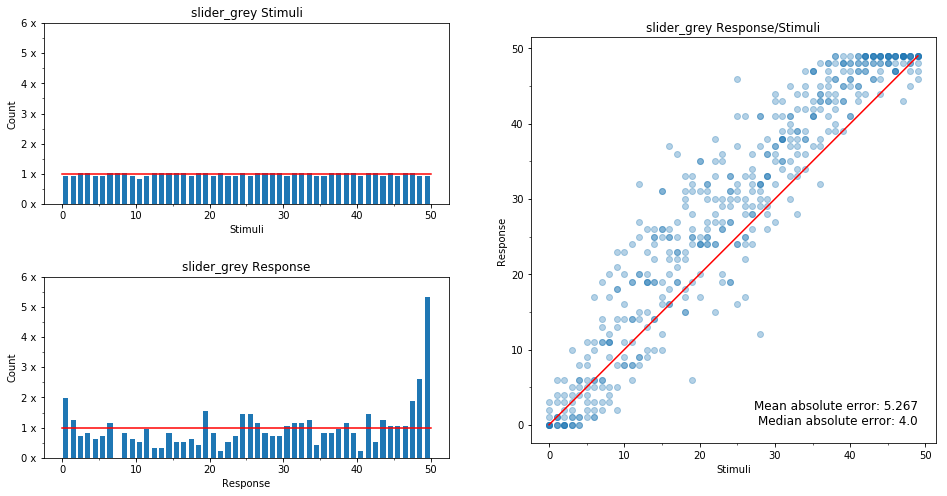
\includegraphics[width=1.2\textwidth]{figures/dist_scatter1.png}
    \caption{Distributions \& scatter plot of stimuli \& responses for slider\_grey}
    \label{dist_scatter1}
\end{figure}

\begin{figure}[p]
    \centering
    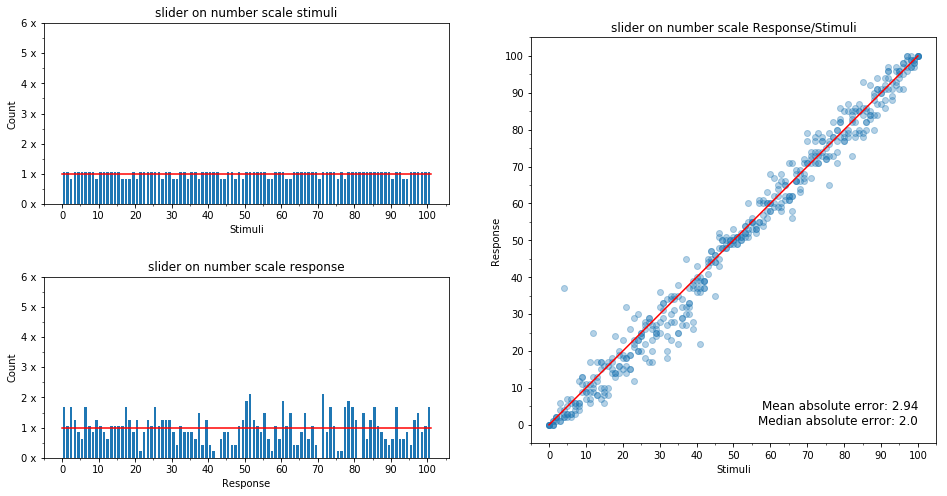
\includegraphics[width=1.2\textwidth]{figures/dist_scatter2.png}
    \caption{Distributions \& scatter plot of stimuli \& responses for slider\_num}
    \label{dist_scatter2}
\end{figure}

\begin{figure}[p]
    \centering
    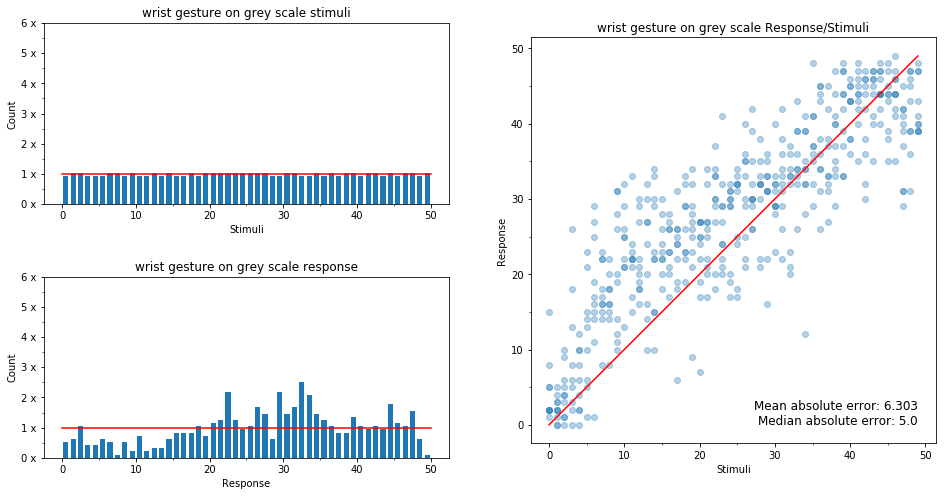
\includegraphics[width=1.2\textwidth]{figures/dist_scatter3.png}
    \caption{Distributions \& scatter plot of stimuli \& responses for wrist\_grey}
    \label{dist_scatter3}
\end{figure}

\begin{figure}[p]
    \centering
    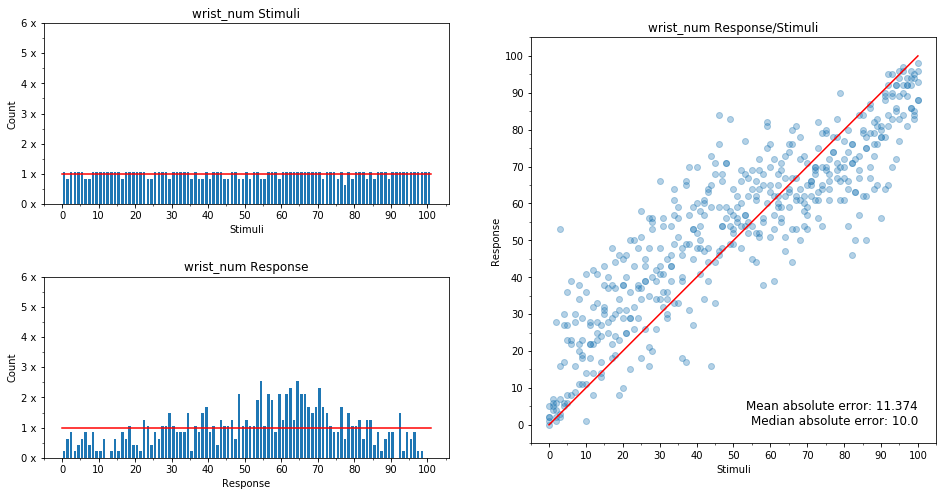
\includegraphics[width=1.2\textwidth]{figures/dist_scatter4.png}
    \caption{Distributions \& scatter plot of stimuli \& responses for wrist\_num}
    \label{dist_scatter4}
\end{figure}

\begin{figure}[p]
    \centering
    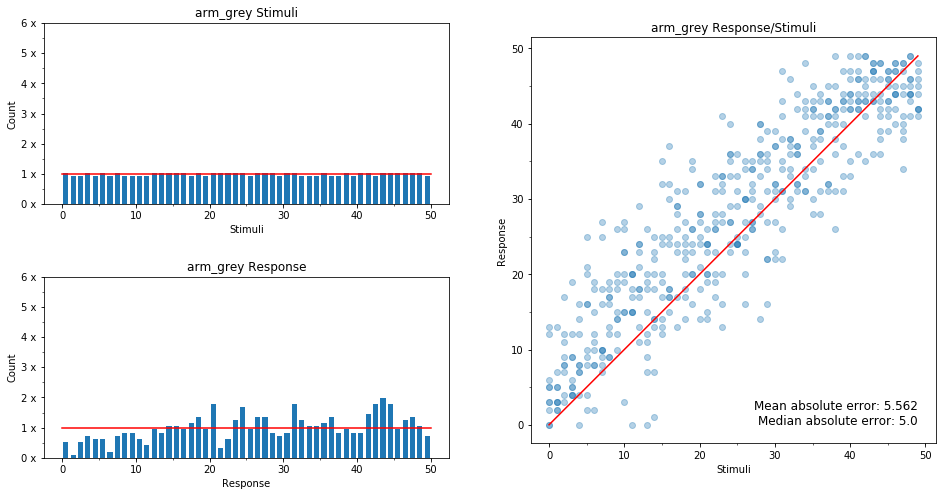
\includegraphics[width=1.2\textwidth]{figures/dist_scatter5.png}
    \caption{Distributions \& scatter plot of stimuli \& responses for arm\_grey}
    \label{dist_scatter5}
\end{figure}

\begin{figure}[p]
    \centering
    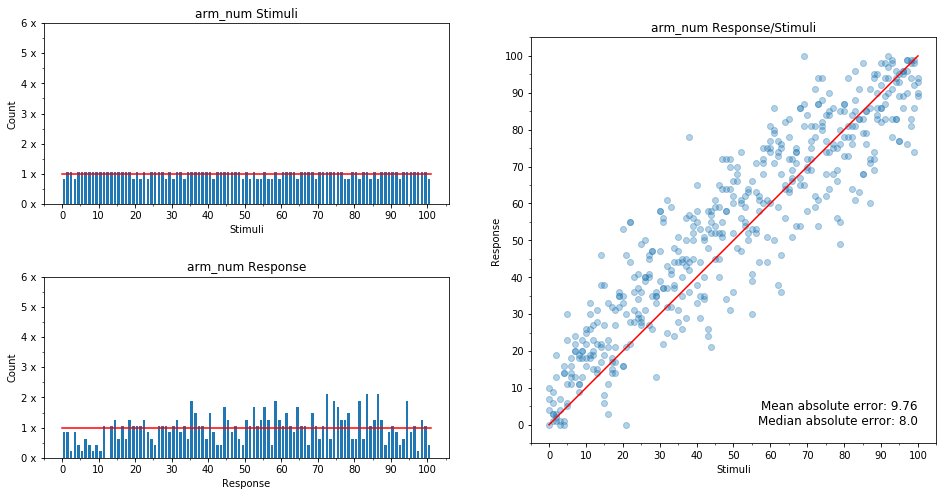
\includegraphics[width=1.2\textwidth]{figures/dist_scatter6.png}
    \caption{Distributions \& scatter plot of stimuli \& responses for arm\_num}
    \label{dist_scatter6}
\end{figure}

First lets investigate the distributions of stimuli and responses. First of all we see that the stimuli is evenly distributed between either 0-49 for the grey exercises or 0-100 for the num exercises, this of course is no surprise since the experiment was designed this way. We do notice that there is a little unevenness in the stimuli distribution, this is due to that each exercise had 24 participants that each performed 20 trials for a total of 480 trials. Neither 50 nor 101 is evenly dividable by this, resulting in a few stimuli being shown one time less than the others. The four outliers removed also influence this, but the overall distribution is as close to even as possible. With the distributions of the responses we don't see a perfect distribution, e.i. completely bias less, but neither do we see a largely skewed distribution meaning there isn't a strong bias. That said there are some interesting observations.

In Matejka et al.\cite{grey} work they find that when using a slider similar to the one used in this experiment, that there was a bias towards the two extremes (min and max) and the middle. In Figure \ref{dist_scatter1} we see a similar bias towards the extremes, and arguably towards the middle, although not as strong a bias as Matejka et al.'s results. They explain that the bias observed was due to the use of a slider (easy for humans to find the middle, and we tend to choose the extremes). But the distribution seen in Figure \ref{dist_scatter2} doesn't show any strong bias, since the only difference of these two exercises is the stimuli (shades of grey vs integers) then these results suggest that the bias observed in both Figure \ref{dist_scatter1} and observed by Matejka et al. is in fact not caused by the slider, but caused by the shades of grey. Looking at the shades of grey in Figure \ref{50shades} it becomes quite apparent, since it is almost impossible to differentiate pure black from the darkest shades. It is a bit easier to tell pure white apart from the light shades, this also explains why the bias toward zero is less significant. Dam-Jensen\cite{dam} found in his results that participants where only able to differentiate around 11 shades of grey, this again explain why the darker shades of grey get registered as pure black by the participants.

In Figure \ref{dist_scatter3} and \ref{dist_scatter4} we see greater amount of responses around the 32 and 65 mark respectively. We will come back to this observation soon.

Looking at the scatter plots we see can see the errors. First of all it is quite clear that the slider\_num exercise outperforms all of the others, the scatter is very close to the diagonal. The other scatters also show a clear correlation around the diagonal, but not as close to it. In Figure \ref{dist_scatter3} and \ref{dist_scatter4} we see a very interesting observation. Looking at the scatters we see that there is a trend, with stimuli at the lower half of the scale the responses are to high and with stimuli in the upper half responses are to low. This is especially clear in Figure \ref{dist_scatter4}. It seems that there is a turning point at approximately 32 and 65 for wrist\_grey and wrist\_num respectively. These turning points are the same as we observed earlier in the distributions. A reasonable explanation for this observation can be found in biology, when investigating the wrist gesture (Figure \ref{roll}) it becomes quite apparent, because of the bone structure in the lower arm (as seen in Figure \ref{bone}) the gesture isn't linear. In the starting position of the gesture the bones are crossed and in the vertical position the bones are parallel. Since the bones aren't the same size and aren't straight this movement becomes non linear, meaning that the amount of movement required to turn the wrist from the starting position till about the halfway point is much greater than the movement needed to turn the wrist from the halfway point to the vertical position. In other words, we have a finer adjustment for the first half of the rotation than we do for the last half. It is plausible that a mathematical model could be created to compensate for this, thus improving this method, but that is beyond the scope of this thesis.

\begin{figure}[h!]
    \centering
    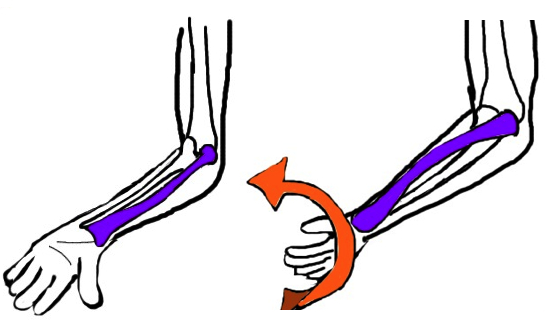
\includegraphics[width=0.5\textwidth]{figures/bone.png}
    \caption{Bone Structure of Lower Arm\cite{bone}}
    \label{bone}
\end{figure}

In Table \ref{abs_error} we see the mean, median and scaled absolute error for each exercise, these are the same values as displayed on the scatter plots. We also see see the amount of data points within $\pm$1 and $\pm$2 on a 0-10 scale, more on this later. The mean and median absolute errors are calculated across all trials for each exercise. The scaled values is the value mapped to a 0-10 scale, this is simply achieved by dividing the value by either 4.9 or 10 respectively for grey and num exercises. We see that for all exercises that the mean and median absolute error is relatively low, when scaled they are all within close to one, meaning on a 0-10 scale the responses fall close to being withing $\pm$1 of the stimuli, of course the exception being the slider\_num which performs even better than the others.

% Please add the following required packages to your document preamble:
% \usepackage{graphicx}
\begin{table}[p]
\centering
\resizebox{\textwidth}{!}{%
\begin{tabular}{rcccccc}
 & \begin{tabular}[c]{@{}c@{}}Mean \\ abs. error\end{tabular} & \begin{tabular}[c]{@{}c@{}}Median \\ abs. error\end{tabular} & \begin{tabular}[c]{@{}c@{}}Scaled mean \\ abs. error\end{tabular} & \begin{tabular}[c]{@{}c@{}}Scaled median \\ abs. error\end{tabular} & \begin{tabular}[c]{@{}c@{}}Points\\ within $\pm$1\end{tabular} & \begin{tabular}[c]{@{}c@{}}Points\\ within $\pm$2\end{tabular} \\ \cline{2-7} 
\multicolumn{1}{r|}{slider\_grey} & \multicolumn{1}{c|}{5.267} & \multicolumn{1}{c|}{4.0} & \multicolumn{1}{c|}{1.075} & \multicolumn{1}{c|}{0.8} & \multicolumn{1}{c|}{51.98\%} & \multicolumn{1}{c|}{79.96\%} \\ \cline{2-7} 
\multicolumn{1}{r|}{slider\_num} & \multicolumn{1}{c|}{2.940} & \multicolumn{1}{c|}{2.0} & \multicolumn{1}{c|}{0.294} & \multicolumn{1}{c|}{0.2} & \multicolumn{1}{c|}{96.04\%} & \multicolumn{1}{c|}{99.58\%} \\ \cline{2-7} 
\multicolumn{1}{r|}{wrist\_grey} & \multicolumn{1}{c|}{6.303} & \multicolumn{1}{c|}{5.0} & \multicolumn{1}{c|}{1.286} & \multicolumn{1}{c|}{1.0} & \multicolumn{1}{c|}{43.22\%} & \multicolumn{1}{c|}{72.03\%} \\ \cline{2-7} 
\multicolumn{1}{r|}{wrist\_num} & \multicolumn{1}{c|}{11.374} & \multicolumn{1}{c|}{10.0} & \multicolumn{1}{c|}{1.137} & \multicolumn{1}{c|}{1.0} & \multicolumn{1}{c|}{48.54\%} & \multicolumn{1}{c|}{79.29\%} \\ \cline{2-7} 
\multicolumn{1}{r|}{arm\_grey} & \multicolumn{1}{c|}{5.563} & \multicolumn{1}{c|}{5.0} & \multicolumn{1}{c|}{1.135} & \multicolumn{1}{c|}{1.0} & \multicolumn{1}{c|}{48.54\%} & \multicolumn{1}{c|}{77.92\%} \\ \cline{2-7} 
\multicolumn{1}{r|}{arm\_num} & \multicolumn{1}{c|}{9.760} & \multicolumn{1}{c|}{8.0} & \multicolumn{1}{c|}{0.976} & \multicolumn{1}{c|}{0.8} & \multicolumn{1}{c|}{55.21\%} & \multicolumn{1}{c|}{88.33\%} \\ \cline{2-7} 
\end{tabular}%
}
\caption{Mean, median and scaled absolute error together with the percentage of points within $\pm$1 and $\pm$2 on the 0-10 scale for each exercise}
\label{abs_error}
\end{table}



To further illustrate how the point in the scatter plots fall based on the 0-10 scale we will add some colored bands to the plots, the green area is where the points fall within $\pm$1, together with the yellow area this is where the points fall within $\pm$2 on the 0-10 scale. On the plots the percentage of point that fall within each area is also displayed (this is also in Table \ref{abs_error}). This is seen in Figure \ref{scatter_color1}, \ref{scatter_color2} and \ref{scatter_color3}. We see that with the exeption of slider\_num that all the other exercises performed about the same, with arm\_num performing just a bit better than the other (with the exeption of slider\_num). Based on the results so far we see no significant different between the three input methods when it comes to rating shades of grey. When rating integers from 0-100 slider\_num strongly outperforms the other two while arm\_num is slightly better than wrist\_num.

\begin{figure}[p]
    \centering
    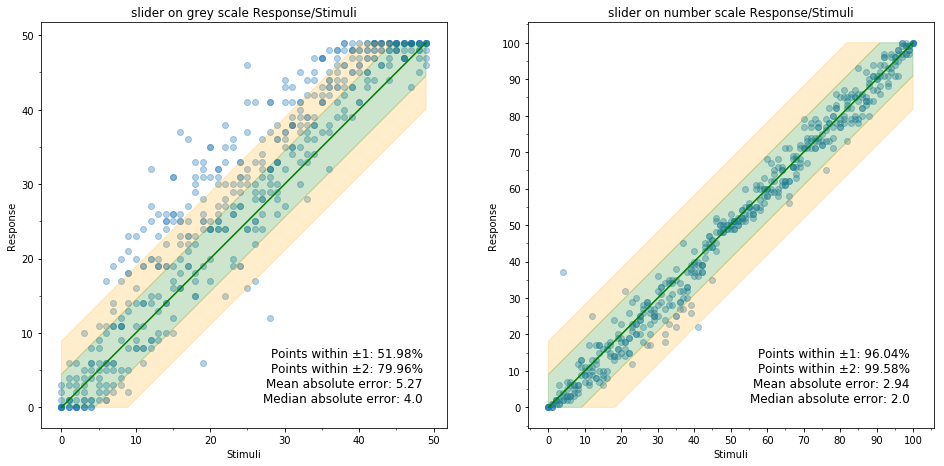
\includegraphics[width=1.15\textwidth]{figures/scatter_col1.png}
    \caption{Scatter plot with color bands for slider}
    \label{scatter_color1}
\end{figure}

\begin{figure}[p]
    \centering
    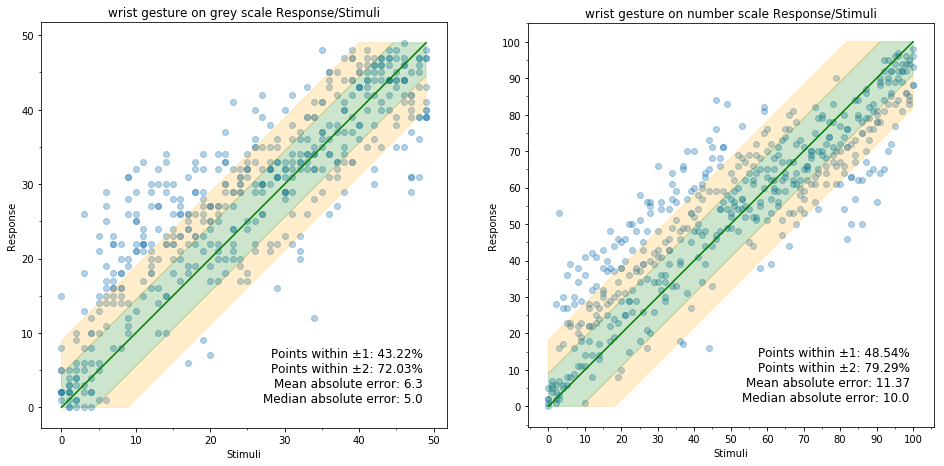
\includegraphics[width=1.15\textwidth]{figures/scatter_col2.png}
    \caption{Scatter plot with color bands for wrist}
    \label{scatter_color2}
\end{figure}

\begin{figure}[p]
    \centering
    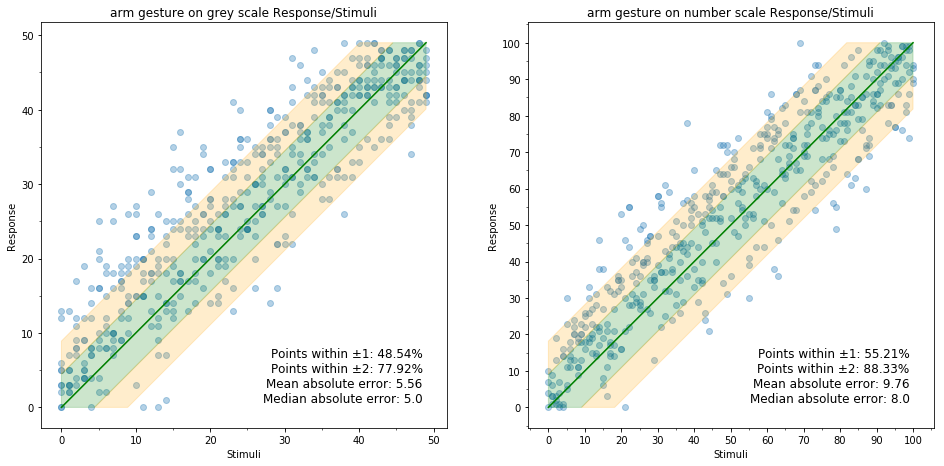
\includegraphics[width=1.15\textwidth]{figures/scatter_col3.png}
    \caption{Scatter plot with color bands for arm}
    \label{scatter_color3}
\end{figure}

\subsection{Error Distribution and Variance}
To further investigate the difference in performance of the different input methods we will look into the error distribution. They will be compared visually and using t-test to see if the are statistically similar. In Figure \ref{error_dist1}, \ref{error_dist2} and \ref{error_dist3} we see the distribution of errors for the six exercises. As we would expect the errors follow a normal distribution centered around zero. Again it is clear to see that the slider\_num performs way better than the other num exercises, the variance is smaller resulting in a much steeper curve meaning that the response are much closer to the stimuli. The other two num exercises (wrist\_num and arm\_num) seem to perform about the same. Likewise all the grey exercises seem to perform about the same, no clear difference in the variance or steepness of the curves.

\begin{figure}[p]
    \centering
    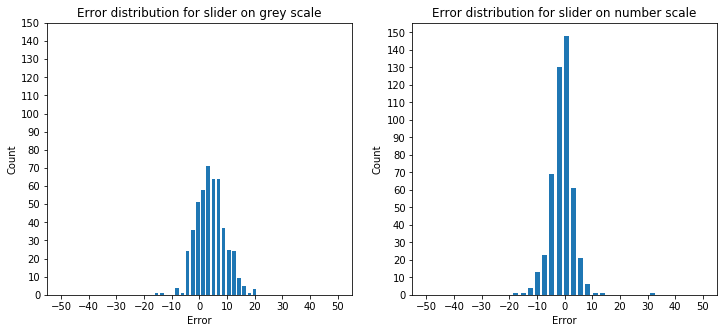
\includegraphics[width=1\textwidth]{figures/error_dist1.png}
    \caption{Error distribution for slider}
    \label{error_dist1}
\end{figure}

\begin{figure}[p]
    \centering
    \includegraphics[width=1\textwidth]{figures/error_dist2.png}
    \caption{Error distribution for wrist}
    \label{error_dist2}
\end{figure}

\begin{figure}[p]
    \centering
    \includegraphics[width=1\textwidth]{figures/error_dist3.png}
    \caption{Error distribution for arm}
    \label{error_dist3}
\end{figure}

T-test where performed between the grey exercises and between the num exercises to see if the are statistically alike. The results of the t-test can be seen in Table \ref{ttest}, for each comparison the errors from all trials of two exercises where used.

Lets start by comparing the grey exercises to each other. We see that wrist\_grey and arm\_grey are quite likely not to have a significant difference. From the results of comparing slider\_grey with wrist\_grey and arm\_grey it is hard to determine weather or not they are similar. On one hand slider\_grey and wrist\_grey is somewhat likely not to be significant different, while slider\_grey and arm\_grey on the other hand are likely to have significant difference. These results are a bit strange, since one would assume if A and B are similar and A and C are different, then B and C must be different too, but here we see that B and C are quite similar (A being slider\_grey, B being wrist\_grey and C being arm\_grey). That being said, the p value for wrist\_grey and arm\_grey is rather high and the calculated t-statistic is close to zero, indicating that this is the most likely case to be true out of the three.

Comparing the num exercises we agian see that there is a clear difference between slide\_num and the other two num exercises. Comparing wrist\_num and arm\_num we see that they are quite similar, meaning that statistically the change of the data being part of the same distribution is high.

Comparing grey exercises to num exercises only makes sence if comparing them with the same input method. Doing so we see the lowest p value and highest calculated t-statistic across the board when comparing slider\_grey to slider\_num, this is not surprising when we know how well slider\_num performed. This indicates that there is a large difference when asked to rate shades of grey using the slider and rate integers using the slider. Both wrist and arm shows to be similar when comparing the grey exercise to the num exercise, and it is quite interesting to see that wrist\_num and wrist\_grey has the highest change of being significant similar across the board. 


With these results we must conclude that the two input methods arm and wrist are quite alike, while we can't say for sure if they are similar to slider when rating shades of grey we can say for curtain that arm and wrist is quite different from slider when rating integers. While the t-test lest us examine the likely hood of two data sets to be similar or not, it can't tell us which performs better.



\begin{table}[]
\centering
\begin{tabular}{cccc}
\multicolumn{2}{c}{Exercises compared} & p value & Calculated t-statistic \\ \hline
\multicolumn{1}{|c|}{slider\_grey} & \multicolumn{1}{c|}{wrist\_grey} & \multicolumn{1}{c|}{0.10045} & \multicolumn{1}{c|}{1.64426} \\ \hline
\multicolumn{1}{|c|}{slider\_grey} & \multicolumn{1}{c|}{arm\_grey} & \multicolumn{1}{c|}{0.01598} & \multicolumn{1}{c|}{2.41378} \\ \hline
\multicolumn{1}{|c|}{wrist\_grey} & \multicolumn{1}{c|}{arm\_grey} & \multicolumn{1}{c|}{0.61034} & \multicolumn{1}{c|}{0.50976} \\ \hline
\multicolumn{1}{l}{} & \multicolumn{1}{l}{} & \multicolumn{1}{l}{} & \multicolumn{1}{l}{} \\ \hline
\multicolumn{1}{|c|}{slider\_num} & \multicolumn{1}{c|}{wrist\_num} & \multicolumn{1}{c|}{1.29468e-10} & \multicolumn{1}{c|}{-6.49960} \\ \hline
\multicolumn{1}{|c|}{slider\_num} & \multicolumn{1}{c|}{arm\_num} & \multicolumn{1}{c|}{9.35024e-19} & \multicolumn{1}{c|}{-9.02859} \\ \hline
\multicolumn{1}{|c|}{wrist\_num} & \multicolumn{1}{c|}{arm\_num} & \multicolumn{1}{c|}{0.39349} & \multicolumn{1}{c|}{-0.85370} \\ \hline
\multicolumn{1}{l}{} & \multicolumn{1}{l}{} & \multicolumn{1}{l}{} & \multicolumn{1}{l}{} \\ \hline
\multicolumn{1}{|c|}{slider\_grey} & \multicolumn{1}{c|}{slider\_num} & \multicolumn{1}{c|}{6.82003e-55} & \multicolumn{1}{c|}{16.65620} \\ \hline
\multicolumn{1}{|c|}{wrist\_grey} & \multicolumn{1}{c|}{wrist\_num} & \multicolumn{1}{c|}{0.93712} & \multicolumn{1}{c|}{0.07892} \\ \hline
\multicolumn{1}{|c|}{arm\_grey} & \multicolumn{1}{c|}{arm\_num} & \multicolumn{1}{c|}{0.14421} & \multicolumn{1}{c|}{-1.46148} \\ \hline
\end{tabular}
\caption{T-test between exercises}
\label{ttest}
\end{table}

Summarizing on the accuracy performance of the three input methods it is quite clear when it comes to rating integers that the slider outperforms both arm and hand. When it comes to rating shades of grey there seems to be no clear significant difference between the three inputs methods. And with the input methods arm and wrist there doesn't seem to be a significant difference in rating shades of grey to rating integers.

\section{Reaction Time}
The reaction time for each trial was recorded, and short analysis showed that there were no significant difference between the six exercises as shown in Table \ref{reaction_time}. There is only a little more than a second difference between the mean reaction time of fastest and slowest exercises. Because of this no further investigation of the reaction time was conducted. The results mean that it doesn't take a significantly longer time to use the wristband than to use the slider, keep in mind that the reaction time was recorded from when stimuli was showed on screen until the participant pressed the submit button. For real life use this gives the wristband a significant advantage, since it wouldn't take much longer to use the wristband in real life than it did in the experiment, but if one where to use a digital VAS on a smartwatch the person would first have to activate the smartwatch and go through the interactions required to input the value This would involve more steps than was present in the experiment, meaning a longer total interaction time.

\begin{table}[]
\centering
\begin{tabular}{rccc}
\multicolumn{1}{c}{} & Mean & Median & \begin{tabular}[c]{@{}c@{}}Standard\\ deviation\end{tabular} \\ \cline{2-4} 
\multicolumn{1}{r|}{slider\_grey} & \multicolumn{1}{c|}{3.589} & \multicolumn{1}{c|}{2.672} & \multicolumn{1}{c|}{2.981} \\ \cline{2-4} 
\multicolumn{1}{r|}{slider\_num} & \multicolumn{1}{c|}{4.552} & \multicolumn{1}{c|}{3.942} & \multicolumn{1}{c|}{2.436} \\ \cline{2-4} 
\multicolumn{1}{r|}{wrist\_grey} & \multicolumn{1}{c|}{4.089} & \multicolumn{1}{c|}{3.195} & \multicolumn{1}{c|}{2.588} \\ \cline{2-4} 
\multicolumn{1}{r|}{wrist\_num} & \multicolumn{1}{c|}{4.376} & \multicolumn{1}{c|}{3.614} & \multicolumn{1}{c|}{2.553} \\ \cline{2-4} 
\multicolumn{1}{r|}{arm\_grey} & \multicolumn{1}{c|}{4.338} & \multicolumn{1}{c|}{3.563} & \multicolumn{1}{c|}{2.522} \\ \cline{2-4} 
\multicolumn{1}{r|}{arm\_num} & \multicolumn{1}{c|}{4.618} & \multicolumn{1}{c|}{3.823} & \multicolumn{1}{c|}{2.633} \\ \cline{2-4} 
\end{tabular}
\caption{Reaction time (seconds) for each exercise}
\label{reaction_time}
\end{table}



\section{Post Experiment Survey}
After the experiment the participants were asked to fill in a survey, the full survey and all the answers can be found in Appendix \ref{survey}. Unfortunately an unknown error occurred while collecting the answers, resulting in three lost answers. This section will show the results of the most relevant questions.

Given the option between the arm and wrist method the participants where asked which method they preferred, which they felt was more accurate and which they felt was most comfortable. For each question they were also given the option to answer that they felt the same for both methods. The results can be seen in Table \ref{arm_vs_wrist}. Among the participants that preferred the arm method they the common answer to why was that the greater range of motion allowed them to have higher precision. For the participant preferring the wrist the most common reason was that it was more comfortable. For the participant that felt that the arm method was more accurate their reason was that it had more precision, making it easier to make small adjustment. The two participants that felt the wrist was more accurate said that they just felt like it. One participant that felt the methods to be equally accurate explained that the task felt difficult in both cases, but with practice and feedback that one could become accurate when using either method. The many participants that felt that the wrist method was more comfortable explained that it was less hassle, less awkward movement and that they didn't get tired. Among the participant rating the two method equally comfortable their comments was that neither of the methods were uncomfortable to use. 


\begin{table}[]
\centering
\begin{tabular}{rccc}
\multicolumn{1}{c}{} & arm & wrist & equal \\ \cline{2-4} 
\multicolumn{1}{r|}{Preferred} & \multicolumn{1}{c|}{38.1\%} & \multicolumn{1}{c|}{42.9\%} & \multicolumn{1}{c|}{19\%} \\ \cline{2-4} 
\multicolumn{1}{r|}{Accurate} & \multicolumn{1}{c|}{81\%} & \multicolumn{1}{c|}{9.5\%} & \multicolumn{1}{c|}{9.5\%} \\ \cline{2-4} 
\multicolumn{1}{r|}{Comfort} & \multicolumn{1}{c|}{9.5\%} & \multicolumn{1}{c|}{61.9\%} & \multicolumn{1}{c|}{28.6\%} \\ \cline{2-4} 
\end{tabular}
\caption{Answers for arm vs wrist}
\label{arm_vs_wrist}
\end{table}

The participants was asked if they had any prior experience using any kind of wearable devices, and with which devices (it was possible to check multiple devices). The results can be seen in Figure \ref{wearable_experience}. This showed that participants represented a good mixture of experience with wearable devices. 

\begin{figure}[h!]
    \centering
    \includegraphics[width=1\textwidth]{figures/wearable_experience.png}
    \caption{Participants prior experience with wearable devices}
    \label{wearable_experience}
\end{figure}

Lastly the participant had a use case explained, where the had to imagine that they suffered from migraines and that their doctor had asked them to log whenever they had a headache and how severe it was. They where then presented with five different methods to log the headaches (which was described in detail) pen and paper, app on smartphone, app on smartwatch, the arm method or the wrist method. They where then asked to order all the method from most preferred to least preferred, the result can be seen in Figure \ref{preferred_method}. The results clearly show that the participants mostly preferred the wristband over the other methods, with pen and paper being the most disliked method. This question should only be seen as an indication, the question required the participants to think of a complex use case and make decisions on things where they probably don't have every piece of information to in order to take an informed decision. That being said the results shows promise for wristband device using the arm and wrist gestures.

\begin{figure}[h!]
    \centering
    \includegraphics[width=1\textwidth]{figures/preferred_method.png}
    \caption{Rating of preferred method (1 is most preferred, 5 is least preferred)}
    \label{preferred_method}
\end{figure}

Based on all of the results, both from the experiment and the survey, is shows great promise for a use case for the wristband. It was shown that the performance of the wristband did just as good for rating shades of grey which argues it would perform well for recording  psychological events, where their isn't a specific value to record, but instead what the user feels. The arm and wrist methods where shown to perform about the same, therefor either could be recommended. Based on the survey it seems to be a trade off between the feeling of accuracy and comfort, but since it has been shown that their isn't a significant difference in accuracy the wrist method would be preferred to achieve a higher level of comfort.
%\chapter{Discussion}

This is the discussion..

\chapter{Future Work}\label{future_ch}

Todo: introduction to chapter.. 

\section{Improvement to the Experiment}
The experiment conducted was a success, but if anyone was to conduct the experiment again a few improvements could be made. With the design of the slider and submit button the button is positioned in the center below the slider. This had the unintended effect of serving as a reference point for the middle of the slider. Simply changing the position of the submit button to either side of the slider would resolve this. As discussed in the results, we humans are quite good at finding the center of a slider anyway, so this is smaller detail that most likely won't have a significant impact on the outcome.

It would be interesting to see if the results of the experiment is representative of a more general population, so recruiting participants with a broader demographic would give an idea of this. Likewise it would be interesting to see if the observed results will stay the same with a larger data set using more participants. In would also be optimal to increase the number of stimuli for each exercise, although it is a trade off since it could lead to fatigue.

Conducting another experiment where only 11 shades of grey and numbers between 0 and 10 would be of interest, to see how the three input methods would compare in a setting closer to the real life use case. Likewise an experiment without a ground truth could be of interest to compare the three input methods, e.g. where participants are asked to rate pain levels, mood or other psychological events. Such an experiment might be harder to conduct since you would need to provide a stimuli for the psychological events, for pain that could be easy, but might not be ethical. It is also harder to compare the results since there won't exist a ground truth, in this case it would be interesting to see how similar the results would be. Such an experiment could be conducted over a longer period of time, where the participants are asked to use both the digital VAS and one or both of the gestures to rate psychological events.

\section{Case Study}
To further develop the work of this thesis, the next step would be to conduct a case study. This could be done similar to the work of Larsen et al.\cite{eg}, where a patient suffering from PTSD was asked to log whenever he experienced a specific event related to his illness using the smartbutton. The difference here would be that the patient would be asked to rate whenever he/she using the wristband and one of the two gestures (arm or wrist). PTSD is just one example that could be used in a case study, it would be equally interesting to conduct a case study on a patient suffering from migraines, chronic pain, anxiety, panic attacks or any similar condition where the common thing is that it will create value to track whenever the events of their conditions occurred and how severe the events are.

With such a case study it would be interesting to see if the tracking of severeness provides additional value over just tracking when events occur. It would be interesting to investigate the compliance of using the wristband with the hand or wrist gestures compared to the simpler smartbutton.

\section{Improvements to Companion App}
The companion app designed and implemented in this thesis was developed with the intentions to be a MVP, therefor some features where left out, but given more time it would create value to improve the companion app. Visualization of the data collected could make it easier to spot patterns. A simple proposal would be bar plot with days along x-axis and the number of tracked events on the y-axis, the bars could be colored to represent the severeness logged. If a given day had 5 data points with severeness rated at 1, 3, 6, 8 and 9 the bar could be colored with multiple color bands based on a color scale going from green, to yellow to red (like in the Mood tracker \ref{mood}). This is just one suggestion, there exist many papers on how to visualize such data, it is important that the visualization is thoroughly tested on a wide demographic to ensure that it can be understood by the users. Beside a better visual presentation of the collected data, it would be interesting to the location of the observation, while this isn't possible with the wristband device, this can be achieved by synchronizing the time stamps of the logged data to the smartphone location history. This could provide additional value to the treatment process. 

While these are the largest improvement that can be made to the companion some other minor adjustments could be made. In order to use companion app the wristband has to be connected first, this is of course important to program the wristband and import the data from it, but that means the user can't aces the collected data without first connecting the wristband. This is of course a inconvenience, the app should let the user see the collected data and only require the wristband to be connected when importing data or programming the wristband. Improvements could be made to the UI of the app to make it more visually pleasing, but that hasn't been the focus of this thesis. Features such as deleting individual data points would also improve the user experience of the app. 

\section{Investigating the Wrist's Critical Point}
In connection to conducting a case study and improving the companion app it would be reasonable to investigate the conditions surrounding the \say{critical point} of the wrist gesture. As mentioned in the  Chapter Results \& Discussions\ref{res_and_dis}, the \say{critical point} is the condition observed that caused the participant's responses to over estimated both the shades of grey and numbers when they where on the lower half of the scale, and under estimate the responses for the upper half of the scale. As mentioned this is likely do the bone structure of the lower arm causing the movement of the gesture to be non linear. It would be interesting to investigate this further and try to develop a mathematical model to compensate for this. Another approach could investigate the use of machine learning and see if that could compensate for this condition, all though for this to be successful a larger data set would most likely be required.



\chapter{Conclusion}

This is the conclusion..


Analyzed the problem

Proposed solution

Successfully implemented wristband and companion app

Conducted experiment

Results: it works! (good enough at least)

\appendix
\chapter{Code}
All the relevant code for this thesis is hosted on GitHub at the following URL:
\url{https://github.com/TheBatAss/Gesture-Based-Input-Method-for-Wearable}

\section{Proof of Concept}\label{poc_code}
The code for the PoC can be found here:

\url{https://github.com/TheBatAss/Gesture-Based-Input-Method-for-Wearable/tree/master/proofOfConcept}

It consist of Python script \say{demo.py} which creates the GUI and communicates with the Adafruit Feather M0 Adalogger\cite{adalogger} which is controlled by the Arduino script \say{demo.ino}.

\section{Companion App}\label{metawear_macro}
The code for the prototype's companion app \say{MetaWear Macro} can be found here:
\url{https://github.com/TheBatAss/Gesture-Based-Input-Method-for-Wearable/tree/master/MetaWear-Macro}

\section{Experiement App}\label{metawear_experiment}
The code for the app \say{MetaWear Experiment} conduction the experiement can be found here:
\url{https://github.com/TheBatAss/Gesture-Based-Input-Method-for-Wearable/tree/master/MetaWear-Experiment}






























\chapter{Survey}\label{survey}
Post experiment survey

Here the questions and answers from the survey will be











\chapter{Experiment App Screens}\label{ex_app_screens}
\begin{figure}[h!]
\centering
\includegraphics[width=0.9\textwidth]{figures/tablet_screen0.png}
\caption{CAPTIONBLABLA}
\label{appendix_app_screen_0}
\end{figure}

\begin{figure}[h!]
\centering
\includegraphics[width=0.9\textwidth]{figures/tablet_screen1.png}
\caption{CAPTIONBLABLA}
\label{appendix_app_screen_1}
\end{figure}

\begin{figure}[h!]
\centering
\includegraphics[width=0.9\textwidth]{figures/tablet_screen2.png}
\caption{CAPTIONBLABLA}
\label{appendix_app_screen_2}
\end{figure}

\begin{figure}[h!]
\centering
\includegraphics[width=0.9\textwidth]{figures/tablet_screen3.png}
\caption{CAPTIONBLABLA}
\label{appendix_app_screen_3}
\end{figure}

\begin{figure}[h!]
\centering
\includegraphics[width=0.9\textwidth]{figures/tablet_screen4.png}
\caption{CAPTIONBLABLA}
\label{appendix_app_screen_4}
\end{figure}

\begin{figure}[h!]
\centering
\includegraphics[width=0.9\textwidth]{figures/tablet_screen5.png}
\caption{CAPTIONBLABLA}
\label{appendix_app_screen_5}
\end{figure}

\begin{figure}[h!]
\centering
\includegraphics[width=0.9\textwidth]{figures/tablet_screen6.png}
\caption{CAPTIONBLABLA}
\label{appendix_app_screen_6}
\end{figure}

\begin{figure}[h!]
\centering
\includegraphics[width=0.9\textwidth]{figures/tablet_screen7.png}
\caption{CAPTIONBLABLA}
\label{appendix_app_screen_7}
\end{figure}

\begin{figure}[h!]
\centering
\includegraphics[width=0.9\textwidth]{figures/tablet_screen8.png}
\caption{CAPTIONBLABLA}
\label{appendix_app_screen_8}
\end{figure}

\begin{figure}[h!]
\centering
\includegraphics[width=0.9\textwidth]{figures/tablet_screen9.png}
\caption{CAPTIONBLABLA}
\label{appendix_app_screen_9}
\end{figure}

\begin{figure}[h!]
\centering
\includegraphics[width=0.9\textwidth]{figures/tablet_screen10.png}
\caption{CAPTIONBLABLA}
\label{appendix_app_screen_10}
\end{figure}

\begin{figure}[h!]
\centering
\includegraphics[width=0.9\textwidth]{figures/tablet_screen11.png}
\caption{CAPTIONBLABLA}
\label{appendix_app_screen_11}
\end{figure}

\begin{figure}[h!]
\centering
\includegraphics[width=0.9\textwidth]{figures/tablet_screen12.png}
\caption{CAPTIONBLABLA}
\label{appendix_app_screen_12}
\end{figure}

\begin{figure}[h!]
\centering
\includegraphics[width=0.9\textwidth]{figures/tablet_screen13.png}
\caption{CAPTIONBLABLA}
\label{appendix_app_screen_13}
\end{figure}

\begin{figure}[h!]
\centering
\includegraphics[width=0.9\textwidth]{figures/tablet_screen14.png}
\caption{CAPTIONBLABLA}
\label{appendix_app_screen_14}
\end{figure}

\begin{figure}[h!]
\centering
\includegraphics[width=0.9\textwidth]{figures/tablet_screen15.png}
\caption{CAPTIONBLABLA}
\label{appendix_app_screen_15}
\end{figure}

\begin{figure}[h!]
\centering
\includegraphics[width=0.9\textwidth]{figures/tablet_screen16.png}
\caption{CAPTIONBLABLA}
\label{appendix_app_screen_16}
\end{figure}

\begin{figure}[h!]
\centering
\includegraphics[width=0.9\textwidth]{figures/tablet_screen17.png}
\caption{CAPTIONBLABLA}
\label{appendix_app_screen_17}
\end{figure}

\begin{figure}[h!]
\centering
\includegraphics[width=0.9\textwidth]{figures/tablet_screen18.png}
\caption{CAPTIONBLABLA}
\label{appendix_app_screen_18}
\end{figure}                                 %Appendix A
%-----------
% Backmatter
%-----------
\backmatter
\chaptermark{Bibliography}
\renewcommand{\sectionmark}[1]{\markright{#1}}
\sectionmark{Bibliography}
\addcontentsline{toc}{chapter}{Bibliography}        %Force addition of Bibliography to TOC
\bibliographystyle{alpha}                           %Use alpha codes for references
\bibliography{References}                           %Bibliography file called
\end{document}
% % % EOF % % %